% Options for packages loaded elsewhere
\PassOptionsToPackage{unicode}{hyperref}
\PassOptionsToPackage{hyphens}{url}
\PassOptionsToPackage{dvipsnames,svgnames,x11names}{xcolor}
%
\documentclass[
  12pt,
]{book}
\usepackage{amsmath,amssymb}
\usepackage{iftex}
\ifPDFTeX
  \usepackage[T1]{fontenc}
  \usepackage[utf8]{inputenc}
  \usepackage{textcomp} % provide euro and other symbols
\else % if luatex or xetex
  \usepackage{unicode-math} % this also loads fontspec
  \defaultfontfeatures{Scale=MatchLowercase}
  \defaultfontfeatures[\rmfamily]{Ligatures=TeX,Scale=1}
\fi
\usepackage{lmodern}
\ifPDFTeX\else
  % xetex/luatex font selection
\fi
% Use upquote if available, for straight quotes in verbatim environments
\IfFileExists{upquote.sty}{\usepackage{upquote}}{}
\IfFileExists{microtype.sty}{% use microtype if available
  \usepackage[]{microtype}
  \UseMicrotypeSet[protrusion]{basicmath} % disable protrusion for tt fonts
}{}
\makeatletter
\@ifundefined{KOMAClassName}{% if non-KOMA class
  \IfFileExists{parskip.sty}{%
    \usepackage{parskip}
  }{% else
    \setlength{\parindent}{0pt}
    \setlength{\parskip}{6pt plus 2pt minus 1pt}}
}{% if KOMA class
  \KOMAoptions{parskip=half}}
\makeatother
\usepackage{xcolor}
\usepackage{longtable,booktabs,array}
\usepackage{calc} % for calculating minipage widths
% Correct order of tables after \paragraph or \subparagraph
\usepackage{etoolbox}
\makeatletter
\patchcmd\longtable{\par}{\if@noskipsec\mbox{}\fi\par}{}{}
\makeatother
% Allow footnotes in longtable head/foot
\IfFileExists{footnotehyper.sty}{\usepackage{footnotehyper}}{\usepackage{footnote}}
\makesavenoteenv{longtable}
\usepackage{graphicx}
\makeatletter
\def\maxwidth{\ifdim\Gin@nat@width>\linewidth\linewidth\else\Gin@nat@width\fi}
\def\maxheight{\ifdim\Gin@nat@height>\textheight\textheight\else\Gin@nat@height\fi}
\makeatother
% Scale images if necessary, so that they will not overflow the page
% margins by default, and it is still possible to overwrite the defaults
% using explicit options in \includegraphics[width, height, ...]{}
\setkeys{Gin}{width=\maxwidth,height=\maxheight,keepaspectratio}
% Set default figure placement to htbp
\makeatletter
\def\fps@figure{htbp}
\makeatother
\setlength{\emergencystretch}{3em} % prevent overfull lines
\providecommand{\tightlist}{%
  \setlength{\itemsep}{0pt}\setlength{\parskip}{0pt}}
\setcounter{secnumdepth}{5}
\ifLuaTeX
  \usepackage{selnolig}  % disable illegal ligatures
\fi
\usepackage[]{natbib}
\bibliographystyle{plainnat}
\IfFileExists{bookmark.sty}{\usepackage{bookmark}}{\usepackage{hyperref}}
\IfFileExists{xurl.sty}{\usepackage{xurl}}{} % add URL line breaks if available
\urlstyle{same}
\hypersetup{
  pdftitle={Breedbase User Manual},
  pdfauthor={Breedbase team},
  colorlinks=true,
  linkcolor={Maroon},
  filecolor={Maroon},
  citecolor={Blue},
  urlcolor={Blue},
  pdfcreator={LaTeX via pandoc}}

\title{Breedbase User Manual}
\author{Breedbase team}
\date{2025-10-08}

\begin{document}
\maketitle

{
\hypersetup{linkcolor=}
\setcounter{tocdepth}{2}
\tableofcontents
}
\hypertarget{introduction}{%
\chapter*{Introduction}\label{introduction}}


Welcome to the Breedbase manual!

This manual is intended for database users.\\
If you are a developer looking for software implementation details, please visit the developer wiki instead: \url{https://github.com/solgenomics/sgn/wiki}

\hypertarget{basic-website-usage}{%
\chapter{Basic Website Usage}\label{basic-website-usage}}

Breedbase is usually hosted on the cloud and is entirely web-based, with only a browser required to access and use it. The recommended browser is Firefox. To use Breedbase, you or your project will usually need to have your own Breedbase instance. Information how you can obtain your own instance can be obtained from the Breedbase project (\url{https://breedbase.org/}).

Once an instance is set up, the site needs to be configured and some metadata uploaded before you can design, run and analyze trials:

\begin{itemize}
\item
  define user accounts and their access privileges.
\item
  add a trait ontology with the traits that you require.
\item
  add the locations that you use in your breeding program
\item
  add the foundational germplasm and the respective pedigree data
\item
  ``historical'' trial data can be uploaded as needed. Usually more recent trials are prioritized over older trials
\end{itemize}

In this chapter, we will cover how you can manage the user accounts and some basic website features such as lists and how to navigate the menus. The other topics are covered in subsequent chapters. Note that Breedbase instances are highly customizable, and that not every instance of Breedbase will have the same options in the same location. Refer to the site specific documentation, if any, for site specific information.

\hypertarget{creating-a-user-account}{%
\section{Creating a User Account}\label{creating-a-user-account}}

\hypertarget{verifying-first-that-you-do-not-already-have-an-account}{%
\subsection{Verifying first that you do not already have an account}\label{verifying-first-that-you-do-not-already-have-an-account}}

Before creating an account, please verify first that you don't already have an account. You can use ``Search'' menu to check if you already registered as a user.

In the ``Search'' menu, selecting the ``People'' tab and search your name. If nothing is found, proceed with the instructions below. Otherwise, clicking the ``Login'' button. If you have forgotten your password, you can retrieve it by clicking the ``Forgot your password?'' link on the login page.

\hypertarget{creating-a-user-account-1}{%
\subsection{Creating a user account}\label{creating-a-user-account-1}}

On the right of the toolbar, clicking on ``Login.'' It will take you to the login page. On the login page, clicking on the link ``sign up for an account.'' It will take you to the page below:

\begin{center}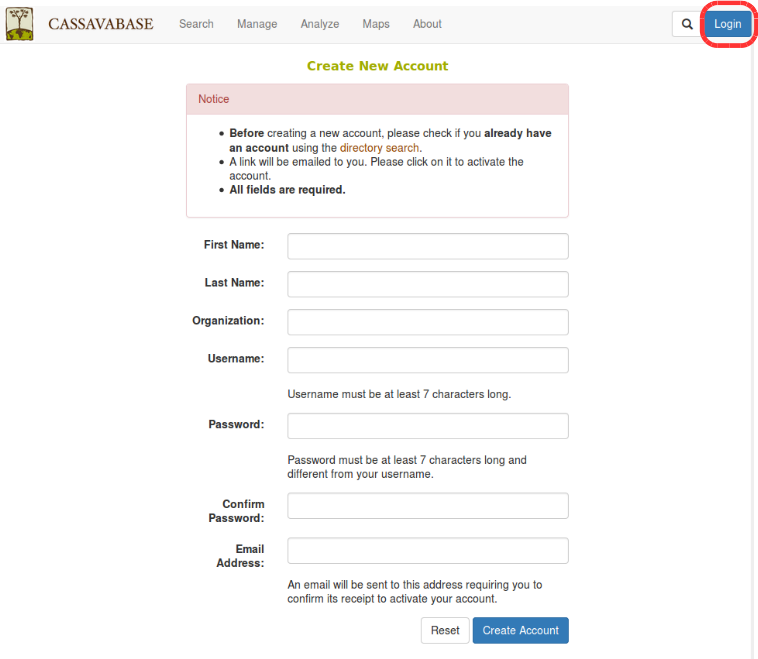
\includegraphics[width=0.95\linewidth]{assets/images/image331} \end{center}

Filling in all of the information, then clicking ``Create Account.''

After you submit the information, an email will be sent to the provided email address. Checking your email and clicking on the link to activate your account.

\hypertarget{managing-your-account}{%
\section{Managing your Account}\label{managing-your-account}}

\hypertarget{login}{%
\subsection{Login}\label{login}}

To login, clicking the ``Login'' link in the toolbar on any page and enter your username and password.

If you have forgotten your password, you can retrieve it by clicking the ``Forgot your password?'' link on the login page.

\begin{center}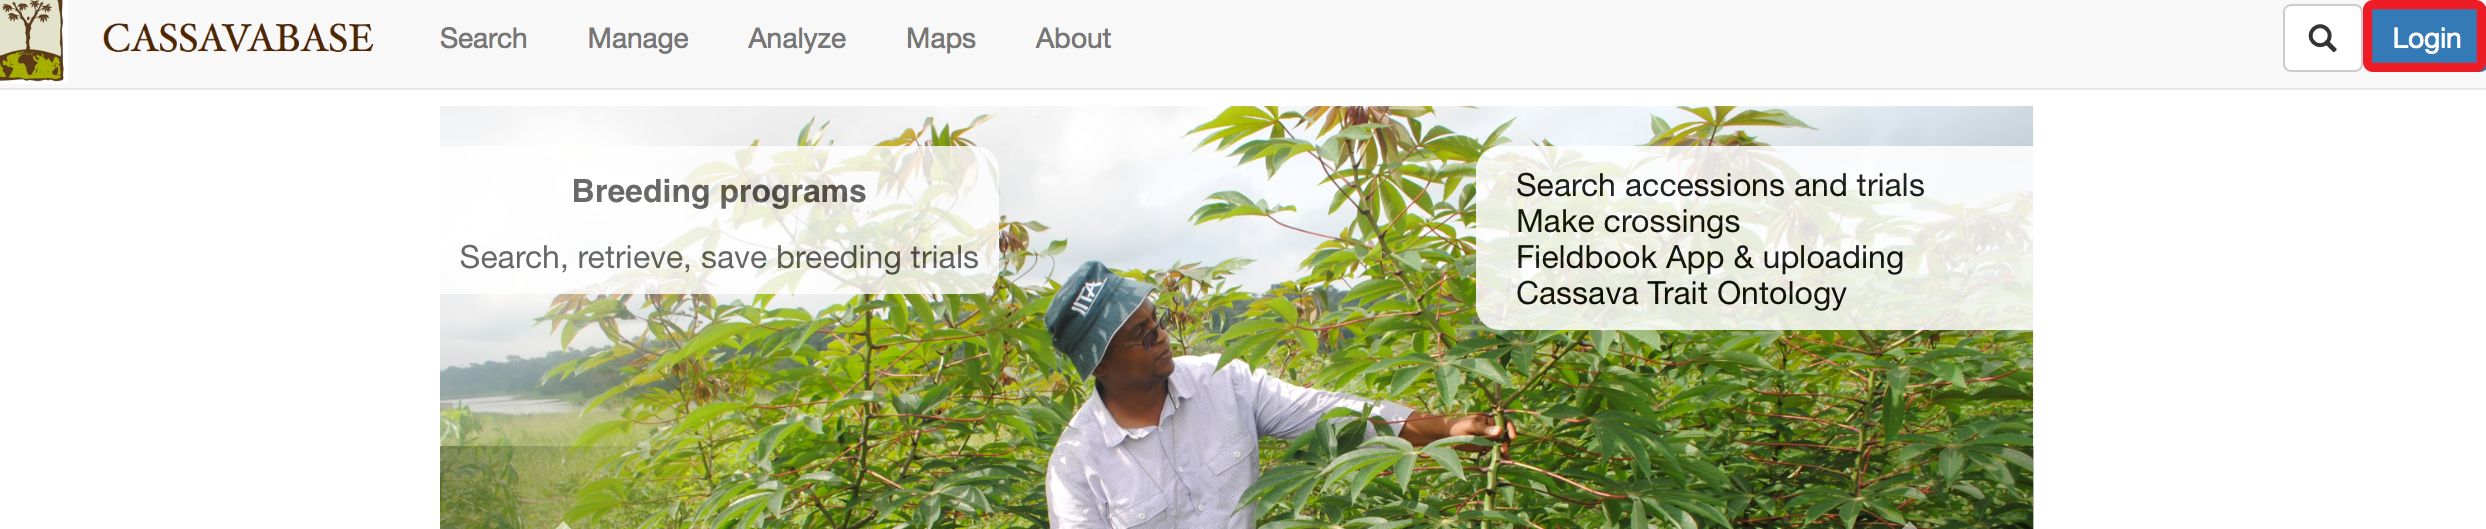
\includegraphics[width=0.95\linewidth]{assets/images/image166} \end{center}

\hypertarget{editing-account-settings}{%
\subsection{Editing Account Settings}\label{editing-account-settings}}

Account settings can be edited by clicking on the ``my profile'' link displayed as your user name, on the right of the toolbar. You must login, in order to access and change account settings.

\begin{center}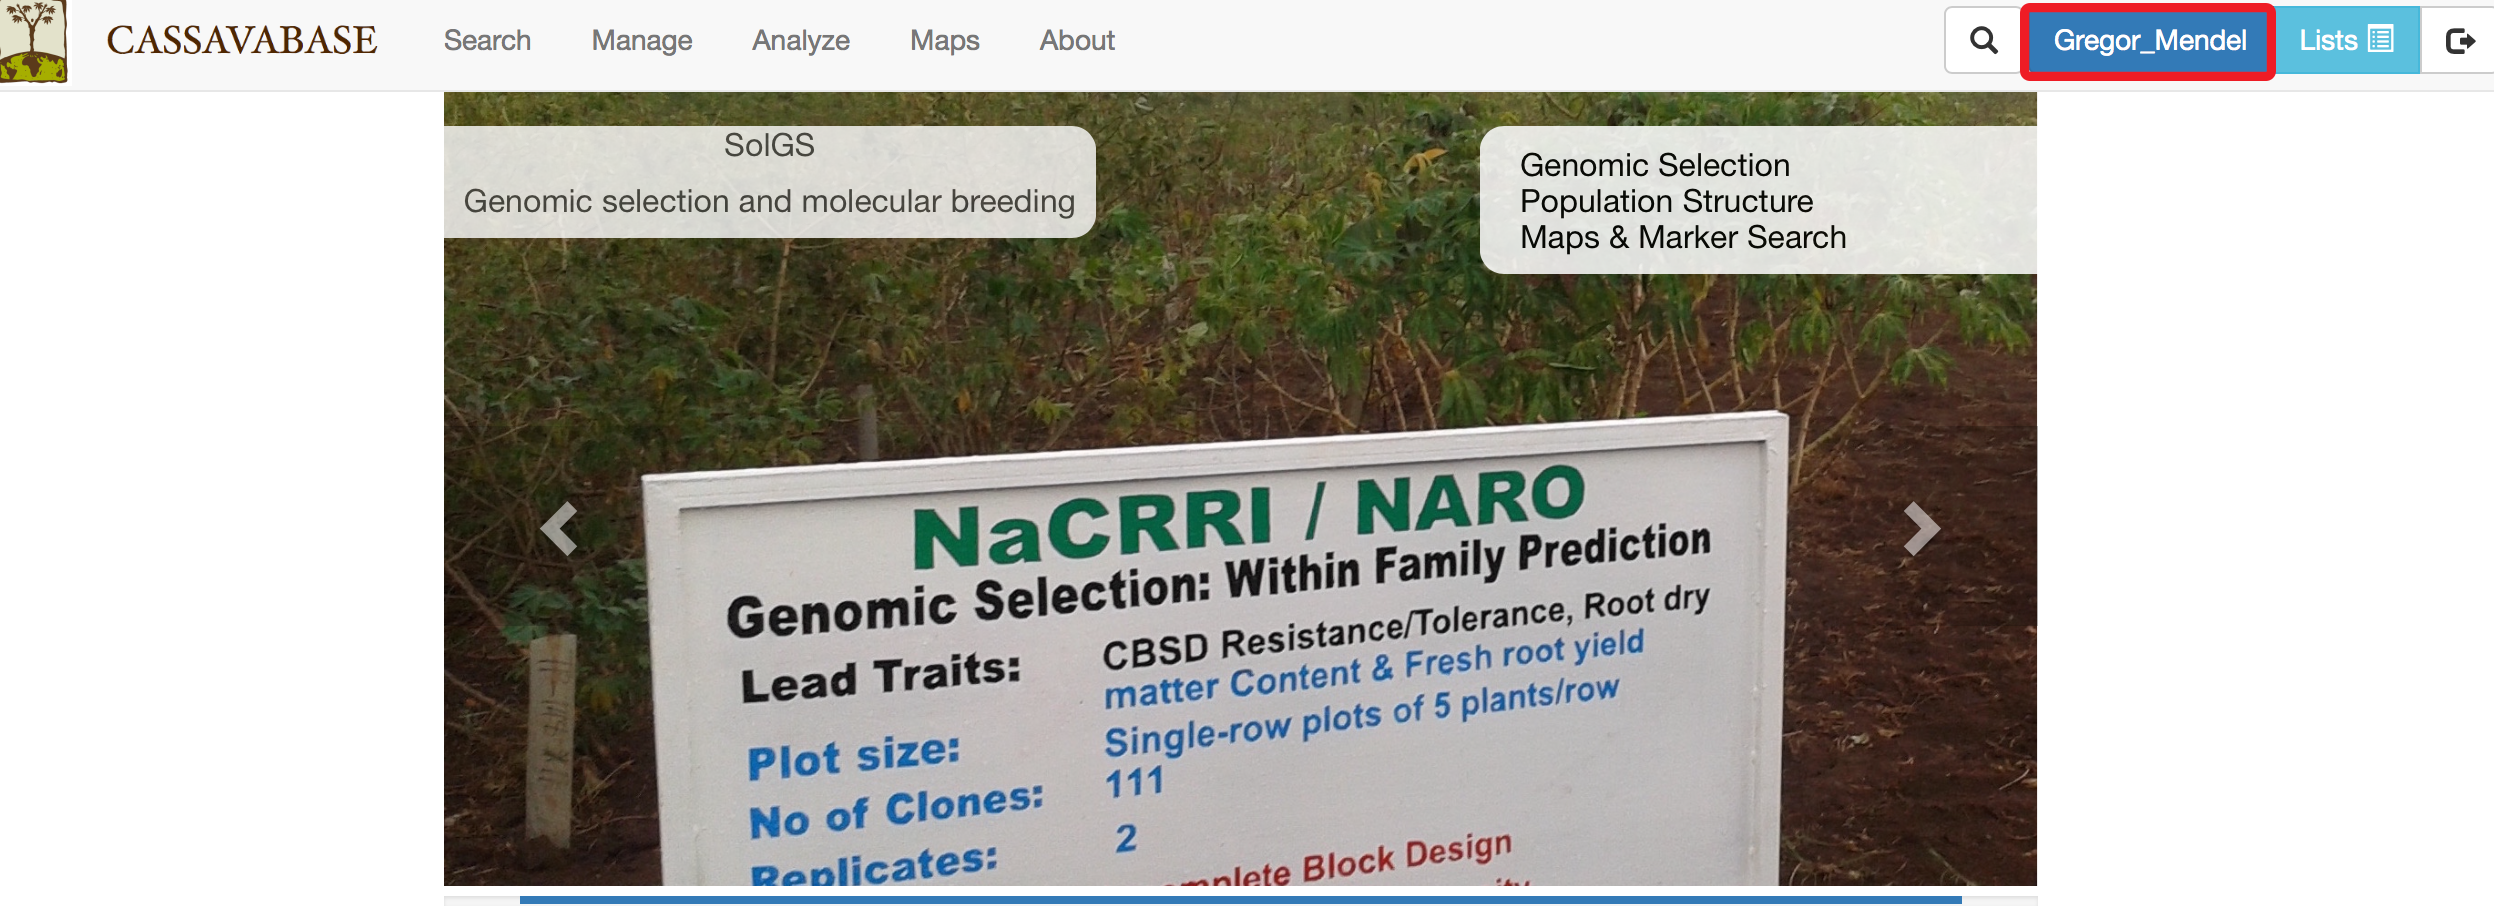
\includegraphics[width=0.95\linewidth]{assets/images/image261} \end{center}

You can add personal information to your account using the ``View or update personal information'' link.

To change your password, username, or your contact email, clicking on ``Update account information'' link. You must provide your old password before you can make any changes.

\begin{center}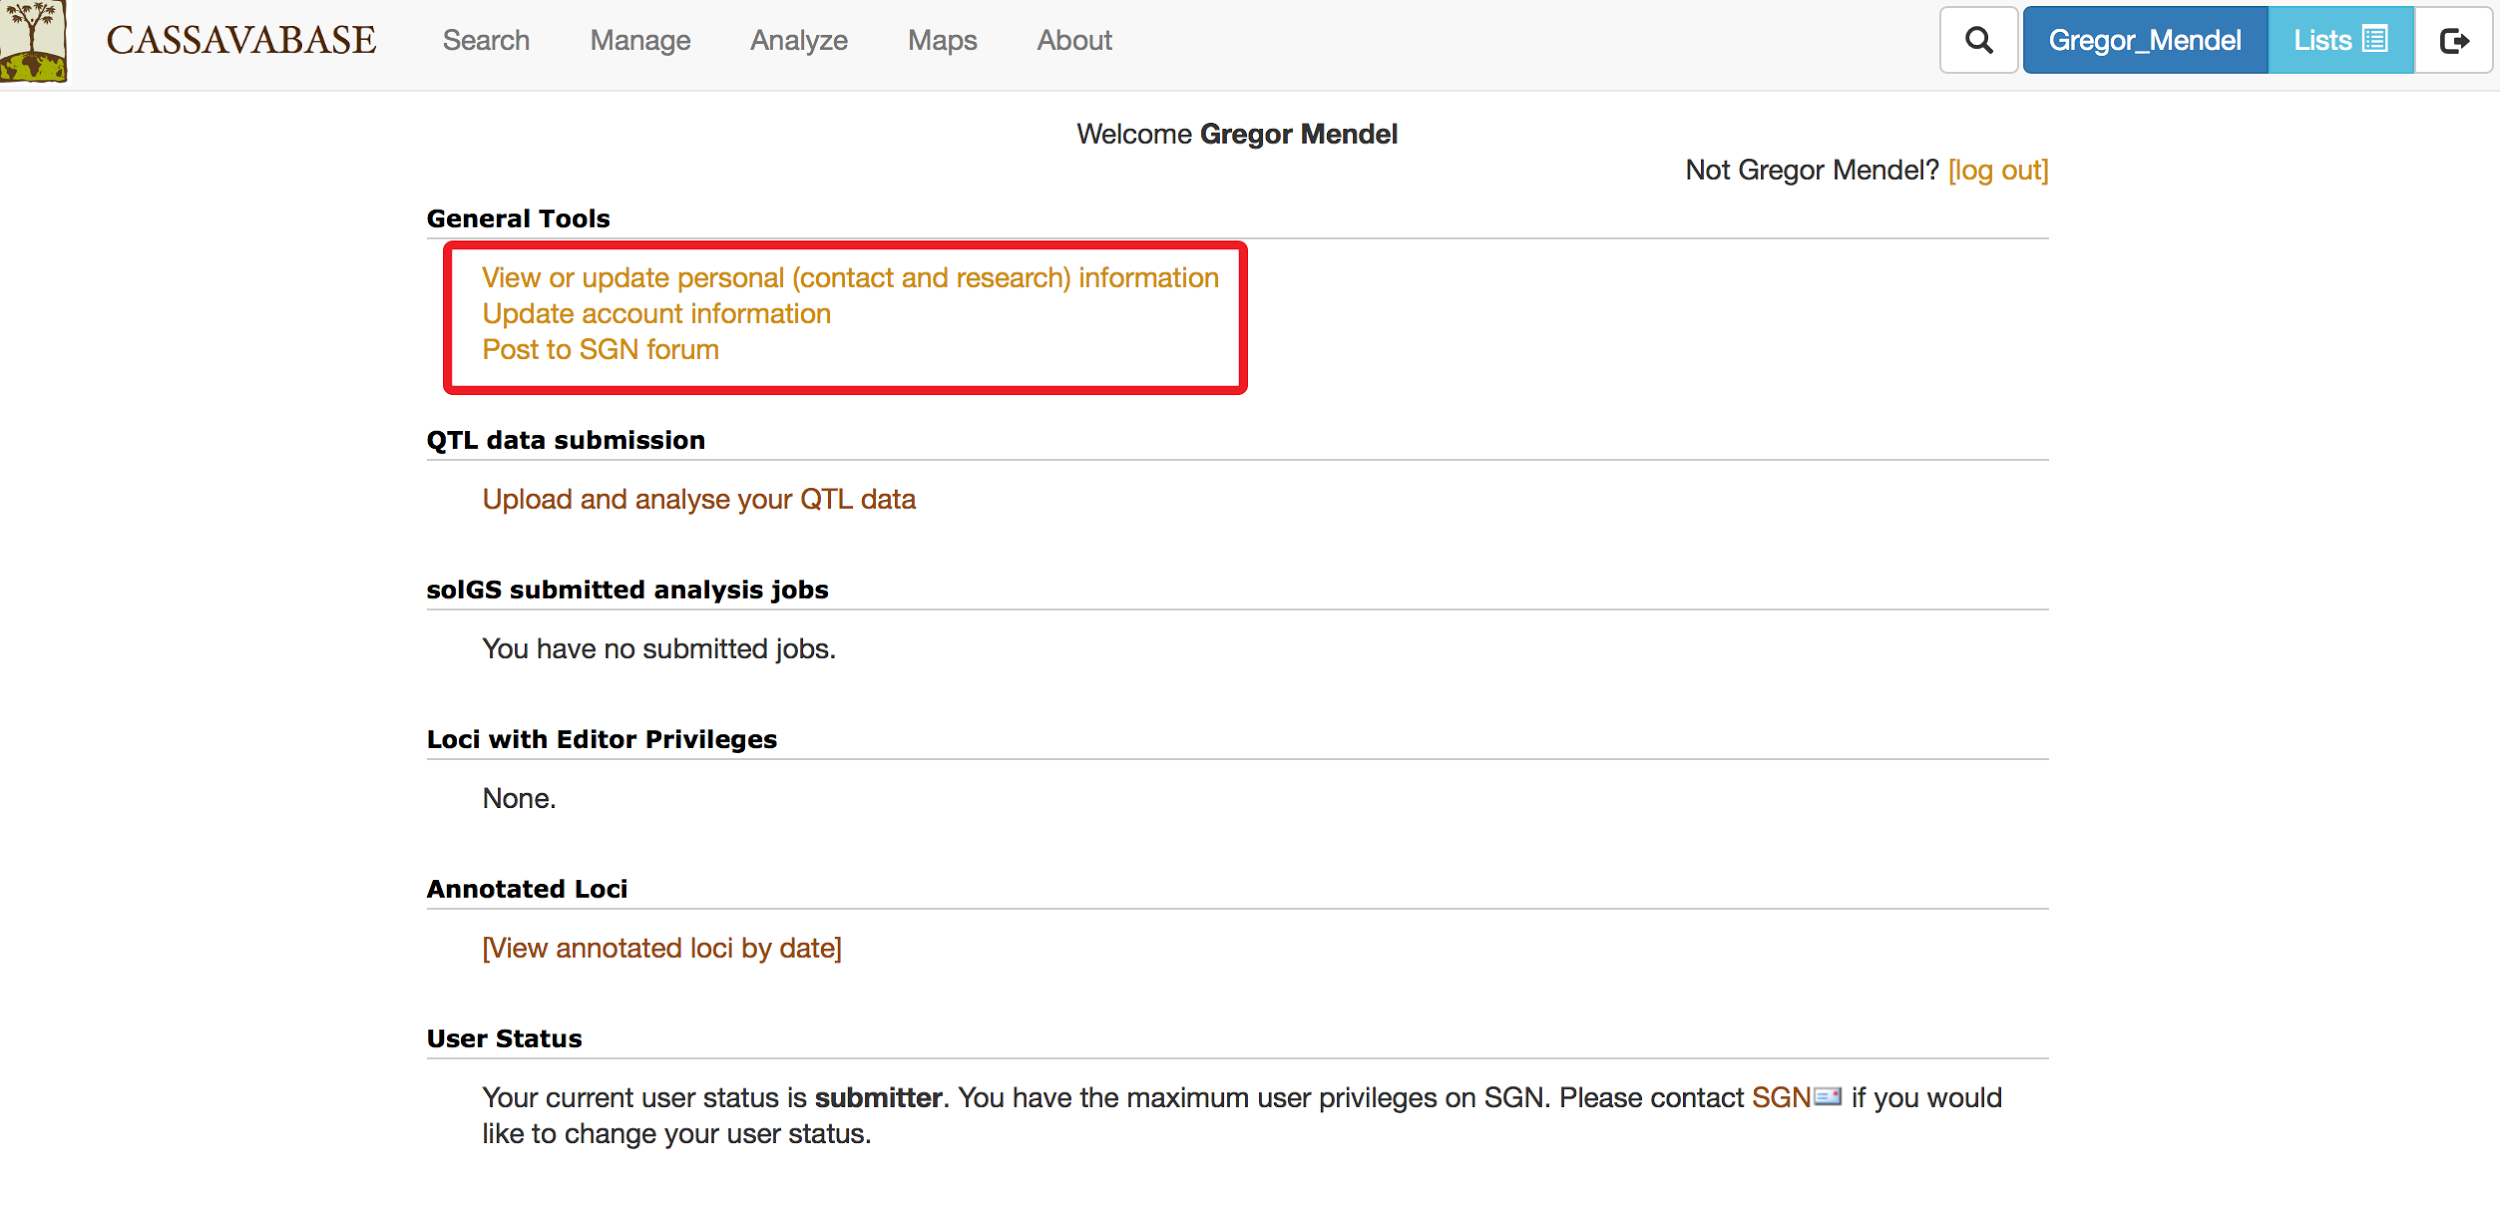
\includegraphics[width=0.95\linewidth]{assets/images/image144} \end{center}

\hypertarget{changing-your-account-status-from-user-to-submitter}{%
\subsection{Changing Your Account Status: From ``User'' to ``Submitter''}\label{changing-your-account-status-from-user-to-submitter}}

After you create an account, your account has a ``user'' status. This account has limited privileges.

Accounts with ``user'' status are able to:

\begin{itemize}
\tightlist
\item
  Change personal information
\item
  Post comments on pages
\item
  Post to the forum
\end{itemize}

To upgrade your account status to ``submitter,'' contact the database curators using the ``contact'' link provided at the footer of each page. Submitter accounts can add data, such as new plots, accessions, phenotype data and images.

\hypertarget{submitting-feedback-on-an-sgn-database}{%
\subsection{Submitting Feedback on an SGN Database}\label{submitting-feedback-on-an-sgn-database}}

We appreciate your feedback! Feel free to submit any questions or suggestions by using the ``Feedback'' link provided at the footer of each page.

\hypertarget{menu-layout}{%
\section{Menu Layout}\label{menu-layout}}

SGN Database websites have a toolbar on the top of each page with a number of menus for convenient access of major functions. The menus, as pictured below, are ``search,'' ``manage,'' ``analyze,'' and ``maps.'' The toolbar also provides a quick search, a ``log in'' button, and a ``new user'' button.

\begin{center}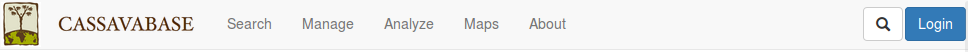
\includegraphics[width=0.95\linewidth]{assets/images/image270} \end{center}

\hypertarget{menu-options}{%
\subsection{Menu Options}\label{menu-options}}

\hypertarget{search}{%
\subsubsection*{Search}\label{search}}


In the Search menu, the options are:

\begin{longtable}[]{@{}
  >{\raggedright\arraybackslash}p{(\columnwidth - 2\tabcolsep) * \real{0.2083}}
  >{\raggedright\arraybackslash}p{(\columnwidth - 2\tabcolsep) * \real{0.7917}}@{}}
\toprule\noalign{}
\begin{minipage}[b]{\linewidth}\raggedright
Tab
\end{minipage} & \begin{minipage}[b]{\linewidth}\raggedright
Description
\end{minipage} \\
\midrule\noalign{}
\endhead
\bottomrule\noalign{}
\endlastfoot
Wizard & Search different accessions and plots by location, year, trial, and trait data. Can also be used to create lists of different types. \\
Accession and plots & Search accessions and plots using a variety of criteria \\
Trials & Search trials by name, description, breeding program, year, location, and trial type. \\
Markers & Search different markers \\
Images & Search images contained in the SGN database \\
People & Search database users \\
\end{longtable}

\hypertarget{manage}{%
\subsubsection*{Manage}\label{manage}}


In the Manage menu, the options are:

\begin{longtable}[]{@{}
  >{\raggedright\arraybackslash}p{(\columnwidth - 2\tabcolsep) * \real{0.2222}}
  >{\raggedright\arraybackslash}p{(\columnwidth - 2\tabcolsep) * \real{0.7778}}@{}}
\toprule\noalign{}
\begin{minipage}[b]{\linewidth}\raggedright
Tab
\end{minipage} & \begin{minipage}[b]{\linewidth}\raggedright
Description
\end{minipage} \\
\midrule\noalign{}
\endhead
\bottomrule\noalign{}
\endlastfoot
Breeding Programs & View, add and delete breeding programs \\
Locations & View, add and delete locations \\
Accessions & Manage and search different accessions \\
Seedlots & Manage and search different seedlots \\
Crosses & Create new crosses in the database \\
Field Trials & Manage field trials. Create trials using different field layouts. \\
Genotyping Plates & Manage genotyping plates. Create 96 or 384 well plates. \\
Phenotyping & Upload phenotyping files from the Tablet Field Book application \\
Field Book App & Manage the field book app data (download files to tablet) \\
Barcodes & Refers to the old barcode system, mainly historical \\
Download & Download information in the database based on lists \\
\end{longtable}

\hypertarget{analyze}{%
\subsubsection*{Analyze}\label{analyze}}


\textbf{Clicking on the ``Analyze'' link will give a full menu of all analysis functions}\\
In the Analyze menu, the options are:

\begin{longtable}[]{@{}
  >{\raggedright\arraybackslash}p{(\columnwidth - 2\tabcolsep) * \real{0.2361}}
  >{\raggedright\arraybackslash}p{(\columnwidth - 2\tabcolsep) * \real{0.7639}}@{}}
\toprule\noalign{}
\begin{minipage}[b]{\linewidth}\raggedright
Tab
\end{minipage} & \begin{minipage}[b]{\linewidth}\raggedright
Description
\end{minipage} \\
\midrule\noalign{}
\endhead
\bottomrule\noalign{}
\endlastfoot
\textbf{Breeder Tools} & \\
Breeder Home & Access breeding functionalities. Lists important and helpful links. \\
Barcode Tools & Manage, create, and download barcodes. Also access barcode tools. \\
Genomic Selection & Can search for traits, start building a GS model, and predict values based on genotypes \\
\textbf{Sequence Analysis} & \\
BLAST & Sequence homology search \\
\textbf{Other} & \\
Ontology Browser & Browse all recorded ontologies \\
\end{longtable}

\hypertarget{working-with-lists}{%
\section{Working with Lists}\label{working-with-lists}}

Lists are collections of identifiers that are stored in the database. Lists can be composed of accessions, plots, traits, locations, and trials. Lists are attached to the individual user's account, and can only be created and seen by the user while logged in. SGN databases make heavy use of lists in a number of tools on the website. For example, trials are created using lists of accessions.

\hypertarget{creating-lists}{%
\subsection{Creating lists}\label{creating-lists}}

Lists can be generated in various ways:

One way to create a list is by clicking on the ``Lists'' link located on the toolbar.

\begin{center}
\includegraphics[width=0.95\linewidth]{assets/images/list_manager_start} \end{center}

To create a new list, enter the name of your new list and then clicking on the ``New List'' button. The name of the list can be anything, but should be unique and should be something to help you easily identify.

\begin{center}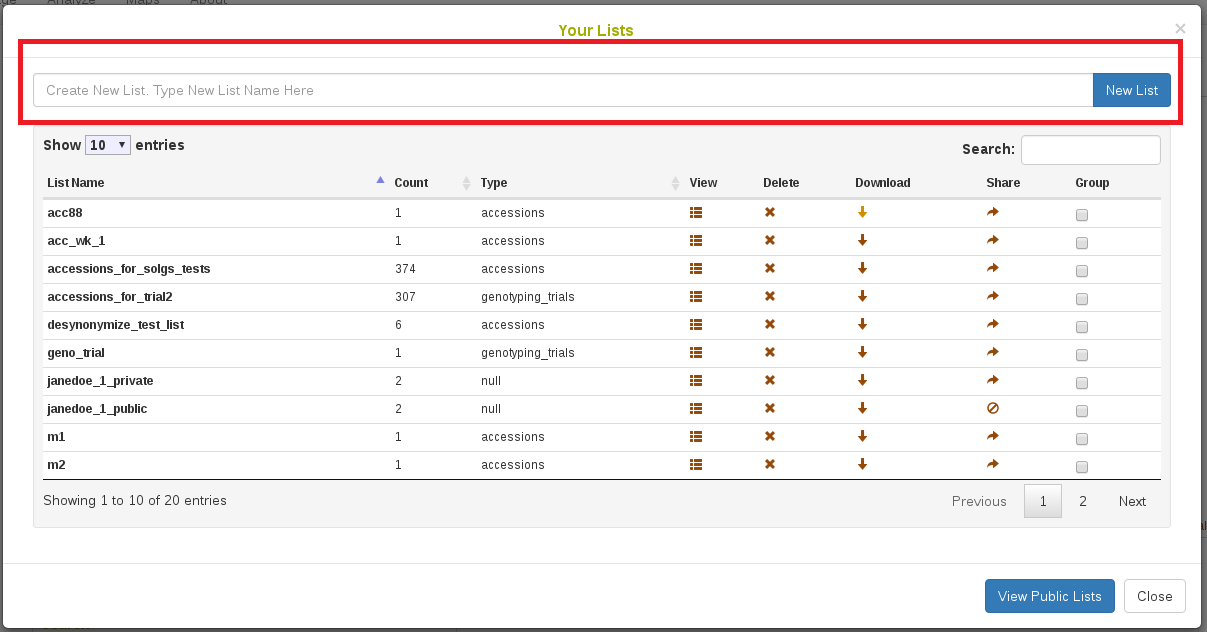
\includegraphics[width=0.95\linewidth]{assets/images/list_manager_new_list} \end{center}

You can find the list that you entered on the ``Your Lists'' page. To add items to your list, click on the ``View'' icon to open ``List Contents'' page.

\begin{center}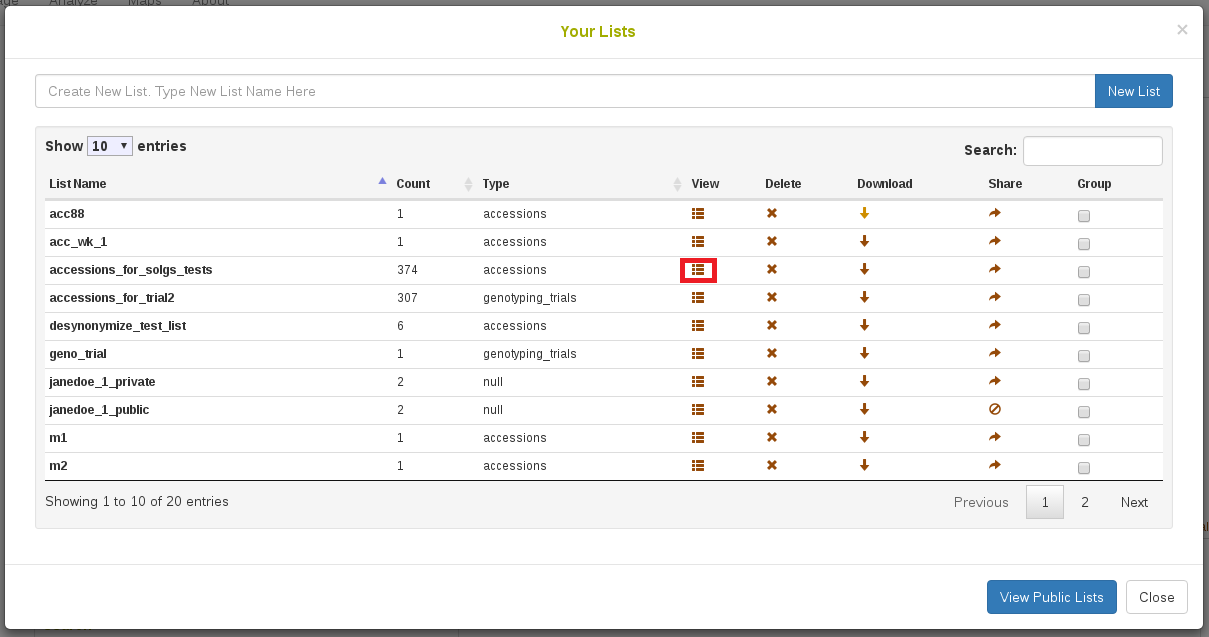
\includegraphics[width=0.95\linewidth]{assets/images/list_manager_view_list} \end{center}

On the ``List Contents'' page, enter items that you want to add to the list, then click on ``Add'' button.

\begin{center}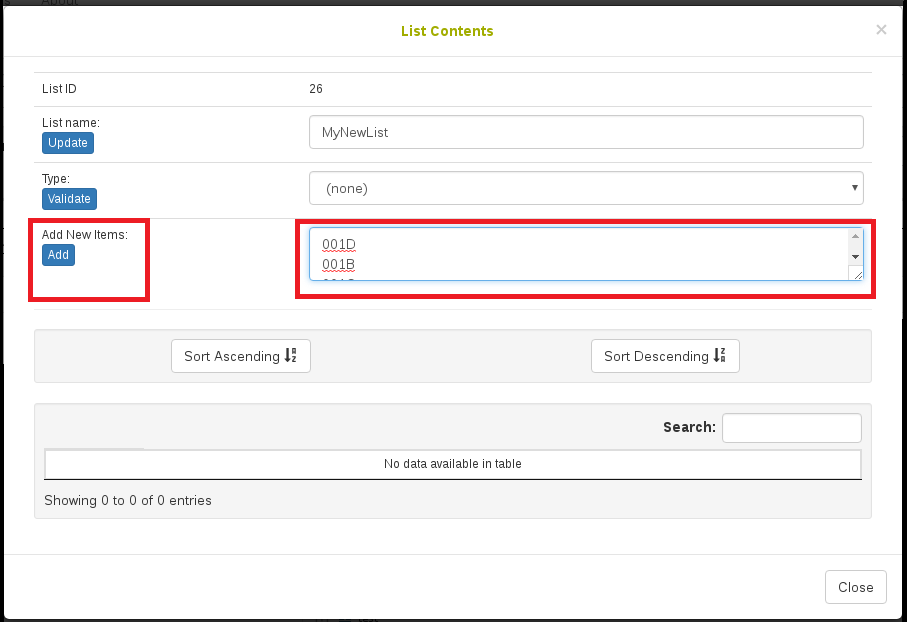
\includegraphics[width=0.95\linewidth]{assets/images/list_manager_add_items} \end{center}

The page will be updated and will display your items in a table at the bottom of the page. It is possible to sort the list if you need.

\begin{center}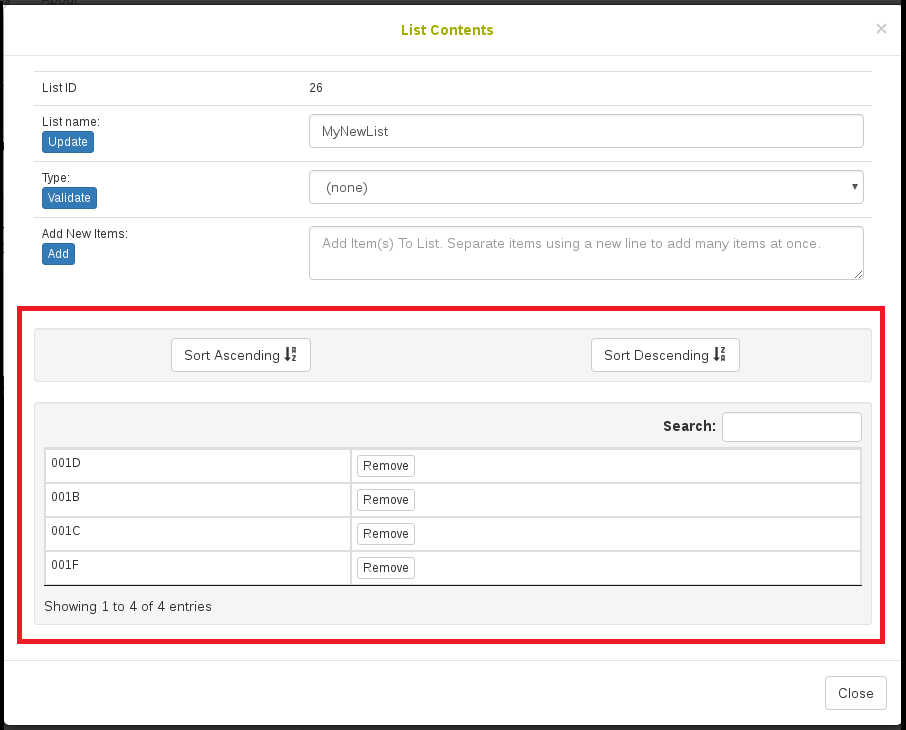
\includegraphics[width=0.95\linewidth]{assets/images/list_manager_added_items} \end{center}

Select the type of items in your list. To verify that the items that you added to your list are already stored in the database and that you selected a correct type for the items, click on the ``Validate'' button.

\begin{center}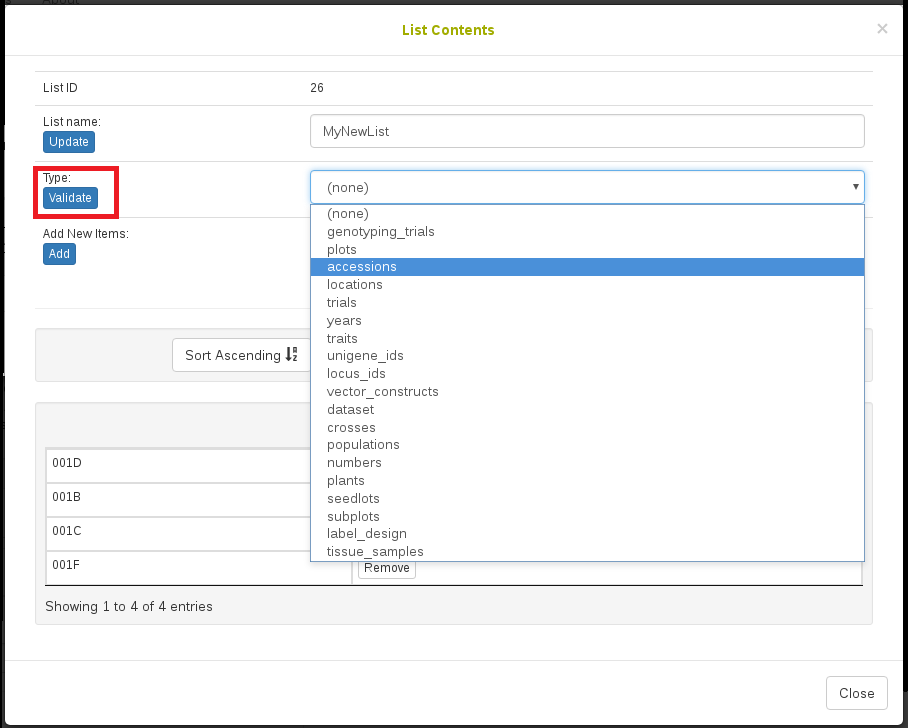
\includegraphics[width=0.95\linewidth]{assets/images/list_manager_list_types} \end{center}

If those items are already in the database, a message will indicate that ``This list passed validation''

\begin{center}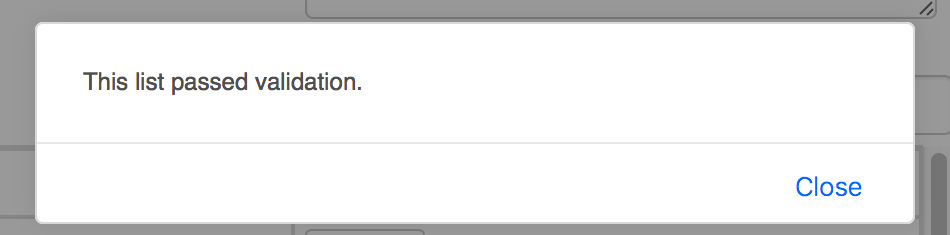
\includegraphics[width=0.5\linewidth]{assets/images/image346} \end{center}

Note that a list cannot contain duplicate elements. If a duplicate item is entered, the list manager will inform the user that the element is already in the list and will not add it again.

Another easy way to create a list is to use \ref{search-wizard}, which can be accessed from the Search menu.

\hypertarget{viewing-and-editing-lists}{%
\subsection{Viewing and editing lists}\label{viewing-and-editing-lists}}

Lists can be viewed and edited using the ``Lists'' link on the toolbar. Clicking on the link will open a window that displays all of your lists, as well as an option to create new lists.

\begin{center}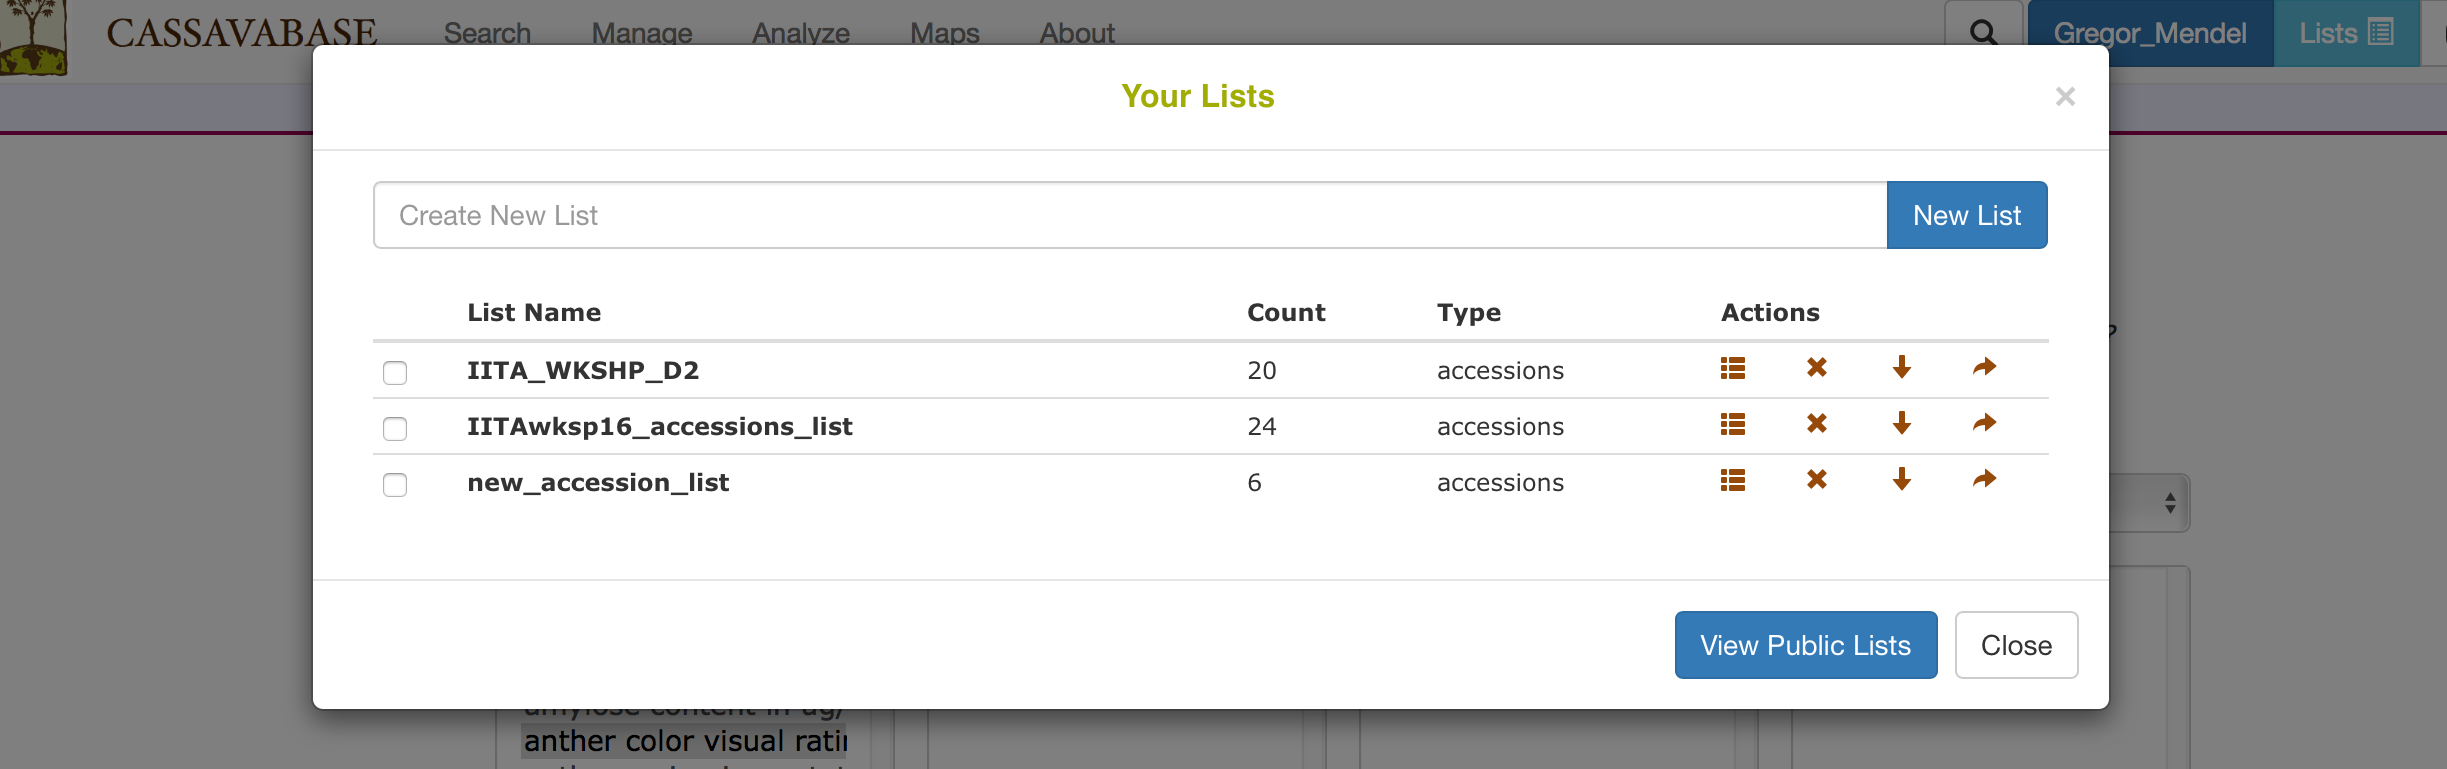
\includegraphics[width=0.95\linewidth]{assets/images/image71} \end{center}

This page shows all lists that have been created, including those created by using the Search Wizard. You can view and edit your lists by using ``Actions'' buttons.

\begin{enumerate}
\def\labelenumi{\arabic{enumi}.}
\item
  Clicking on the ``view'' icon will open a new window called ``List Contents'' that allows you to change the list name, the type of the list, add new items, or delete existing items.
\item
  Clicking on the ``delete'' icon will delete your list. \textbf{Caution: this action cannot be undone}.
\item
  Clicking on the ``download'' icon will download the contents of your list to your computer.
\item
  Clicking on the ``make public'' icon will make your list available for other users to view and use your list.
\end{enumerate}

\begin{center}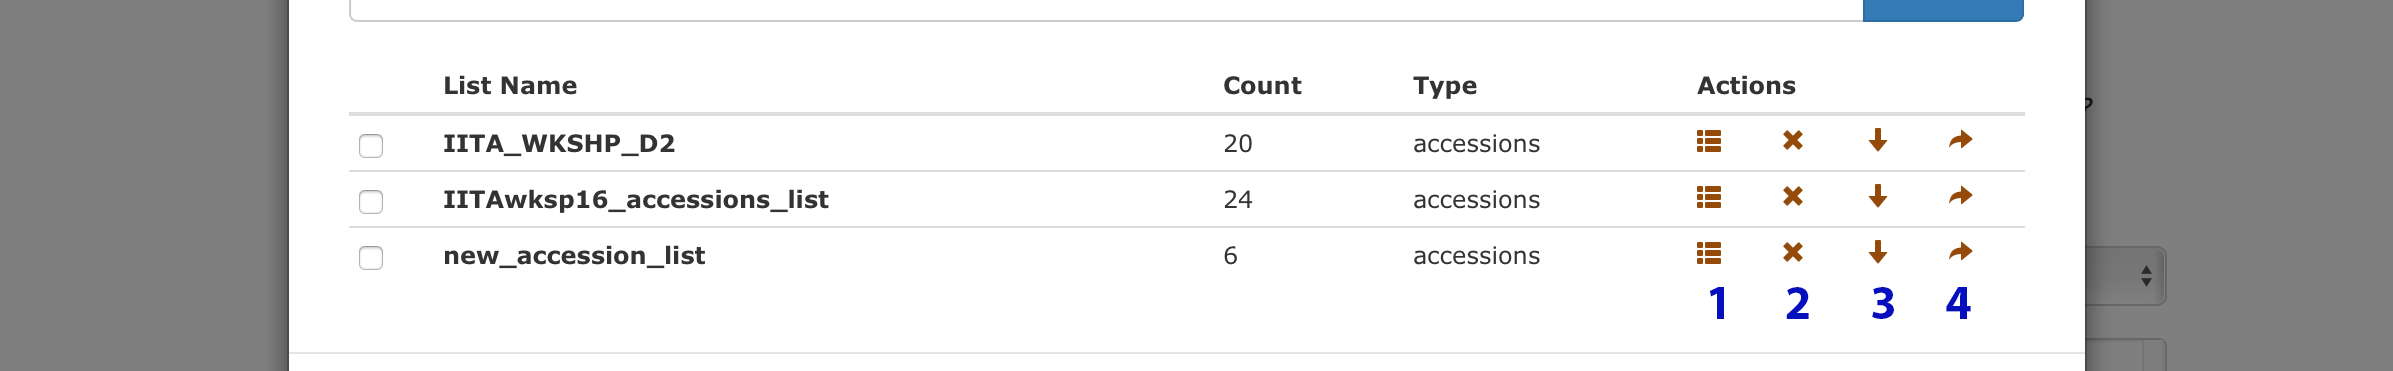
\includegraphics[width=0.95\linewidth]{assets/images/image297} \end{center}

\hypertarget{user-permissions}{%
\section{User Permissions}\label{user-permissions}}

Breedbase accounts are assigned one or more of four different roles to determine the level of access they have within the database. The possible roles are \textbf{User}, \textbf{Submitter}, \textbf{Sequencer}, and \textbf{Curator}. Each role grants specific permissions, and careful management of them helps prevent data from being altered or deleted in error.

\begin{center}
\includegraphics[width=0.5\linewidth]{assets/images/roles} \end{center}

Accounts are also assigned Breeding Program role(s) to grant access to the specfic breeding program(s) they work with.

\begin{itemize}
\tightlist
\item
  The \textbf{User} role gives an account permission to view and download data throughout the database.
\item
  The \textbf{Submitter} role gives an account permission to design field experiments and to upload and edit data using the tools in the ``Manage'' section. In order to submit and manage breeding data within a given breeding program, a submitter also must have a matching Breeding Program role.
\item
  The \textbf{Sequencer} role gives an account permission to design genotyping experiments and submit plates to a genotyping service.
\item
  The \textbf{Curator} role gives an account permission to do all of the above, as well as to delete data within the database. The Curator role also enables the addition or deletion of roles for all database accounts in the `Manage User Roles' tool.
\end{itemize}

\hypertarget{searching-the-database}{%
\chapter{Searching the Database}\label{searching-the-database}}

You can search for information on the database by using the following search options: Wizard, which uses combined criteria specified by users; Accessions and Plots; Trials; Markers; Images; People; FAQ.

\begin{center}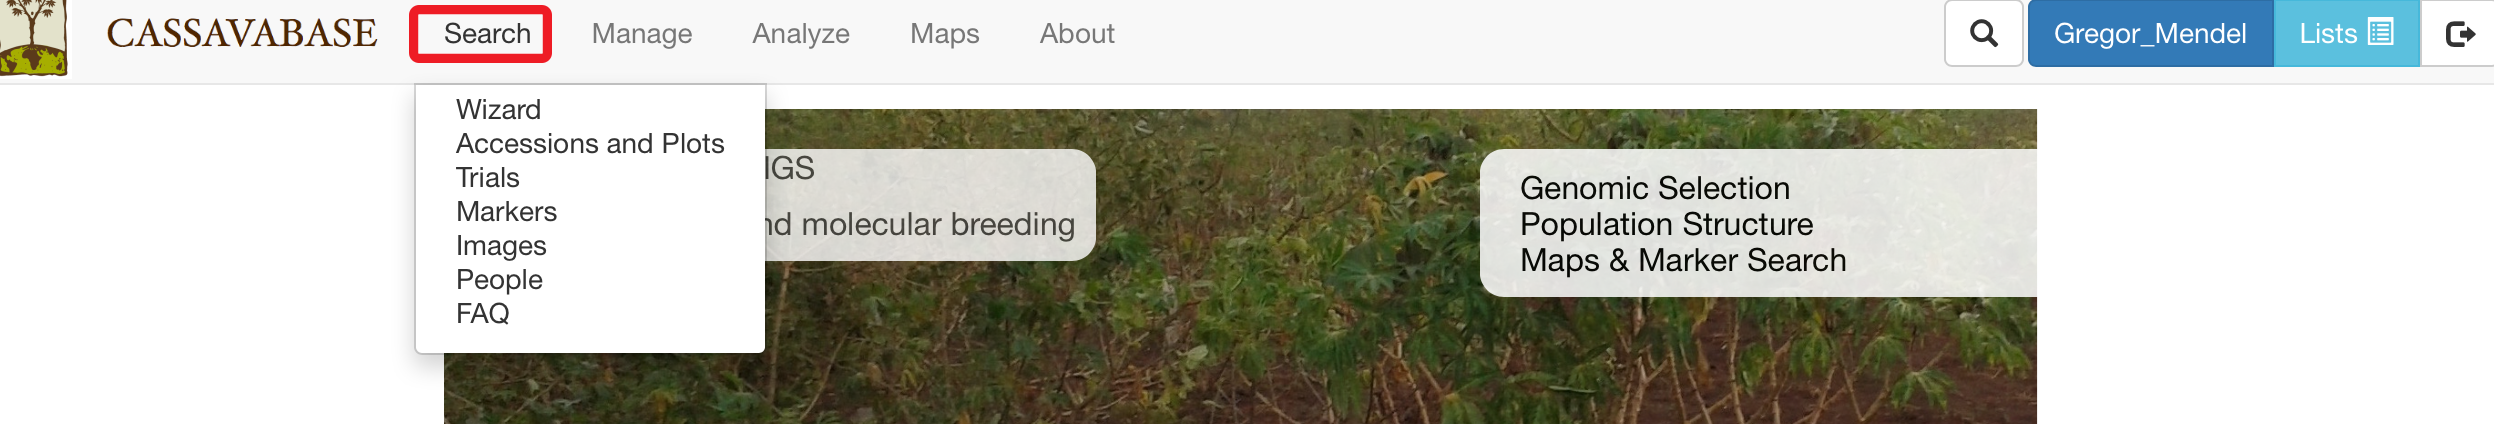
\includegraphics[width=0.95\linewidth]{assets/images/image267} \end{center}

\hypertarget{search-wizard}{%
\section{The Search Wizard}\label{search-wizard}}

\begin{center}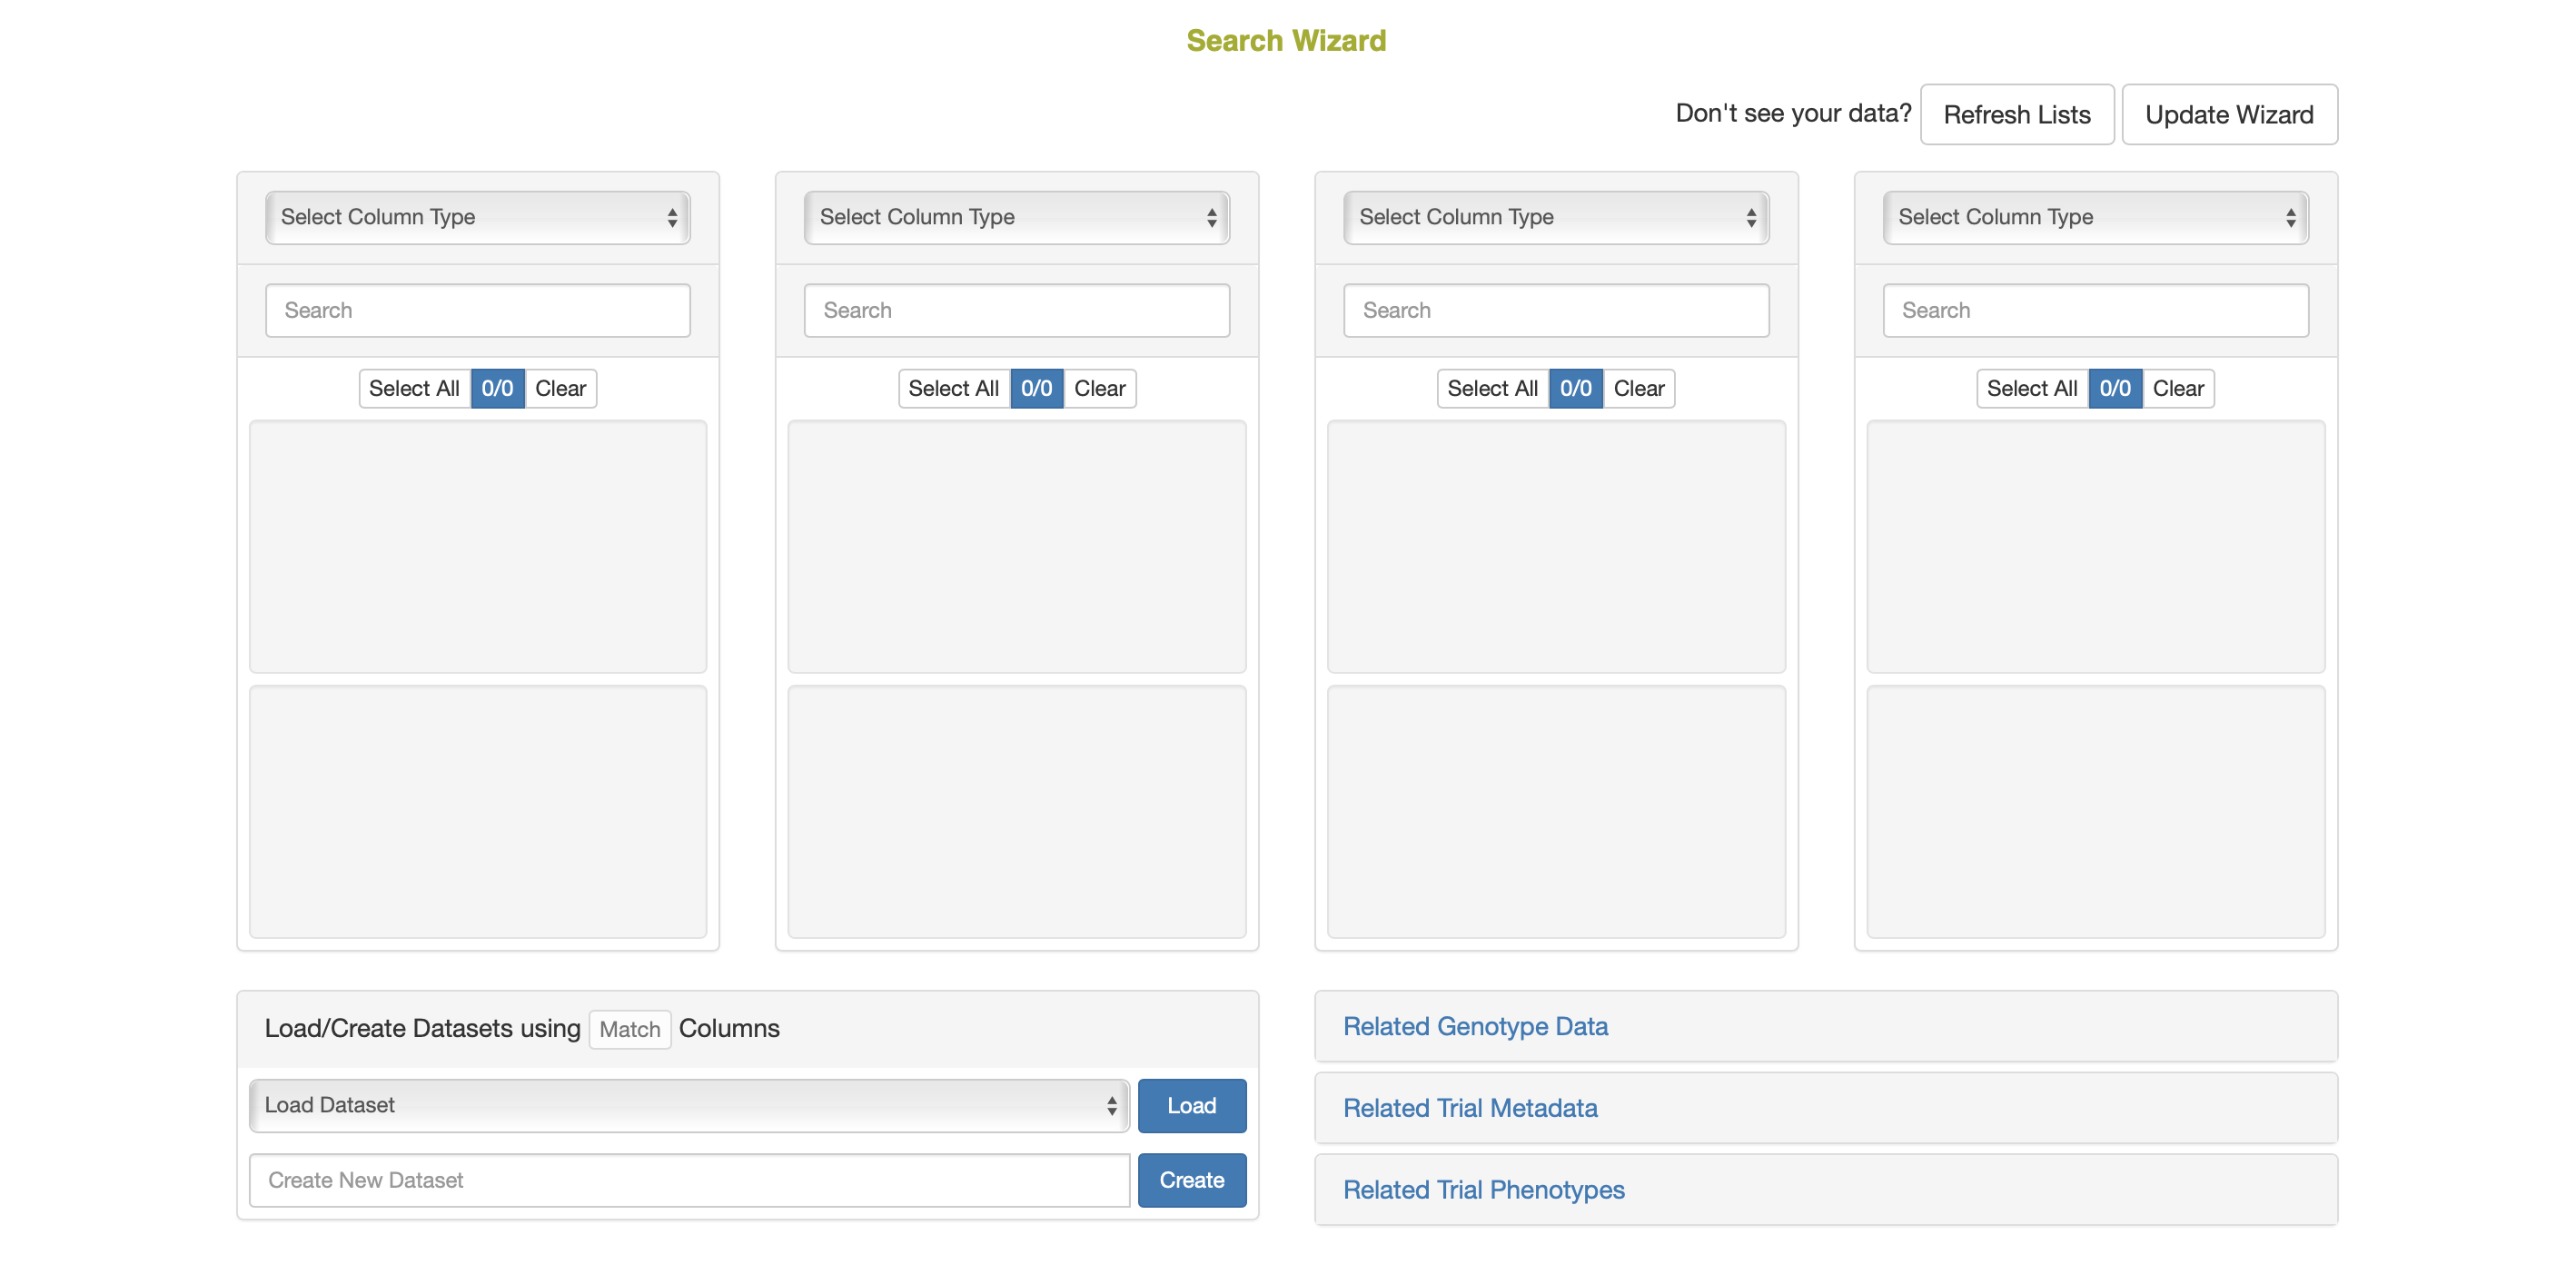
\includegraphics[width=0.95\linewidth]{assets/images/wizard_interface} \end{center}

\hypertarget{how-the-search-wizard-works}{%
\subsection{How the Search Wizard Works}\label{how-the-search-wizard-works}}

The search wizard presents a number of select boxes, which are initially empty. You start searching by picking a category of data from the dropdown above the left-most select box.

Once a category has been picked, the database will retrieve all the options within this category and display them within the first select box. You then select one or more options from the first select box, which activates the second dropdown.

You can then select a category from the second dropdown, and repeat this same search process through all four dropdowns and select boxes.

\begin{center}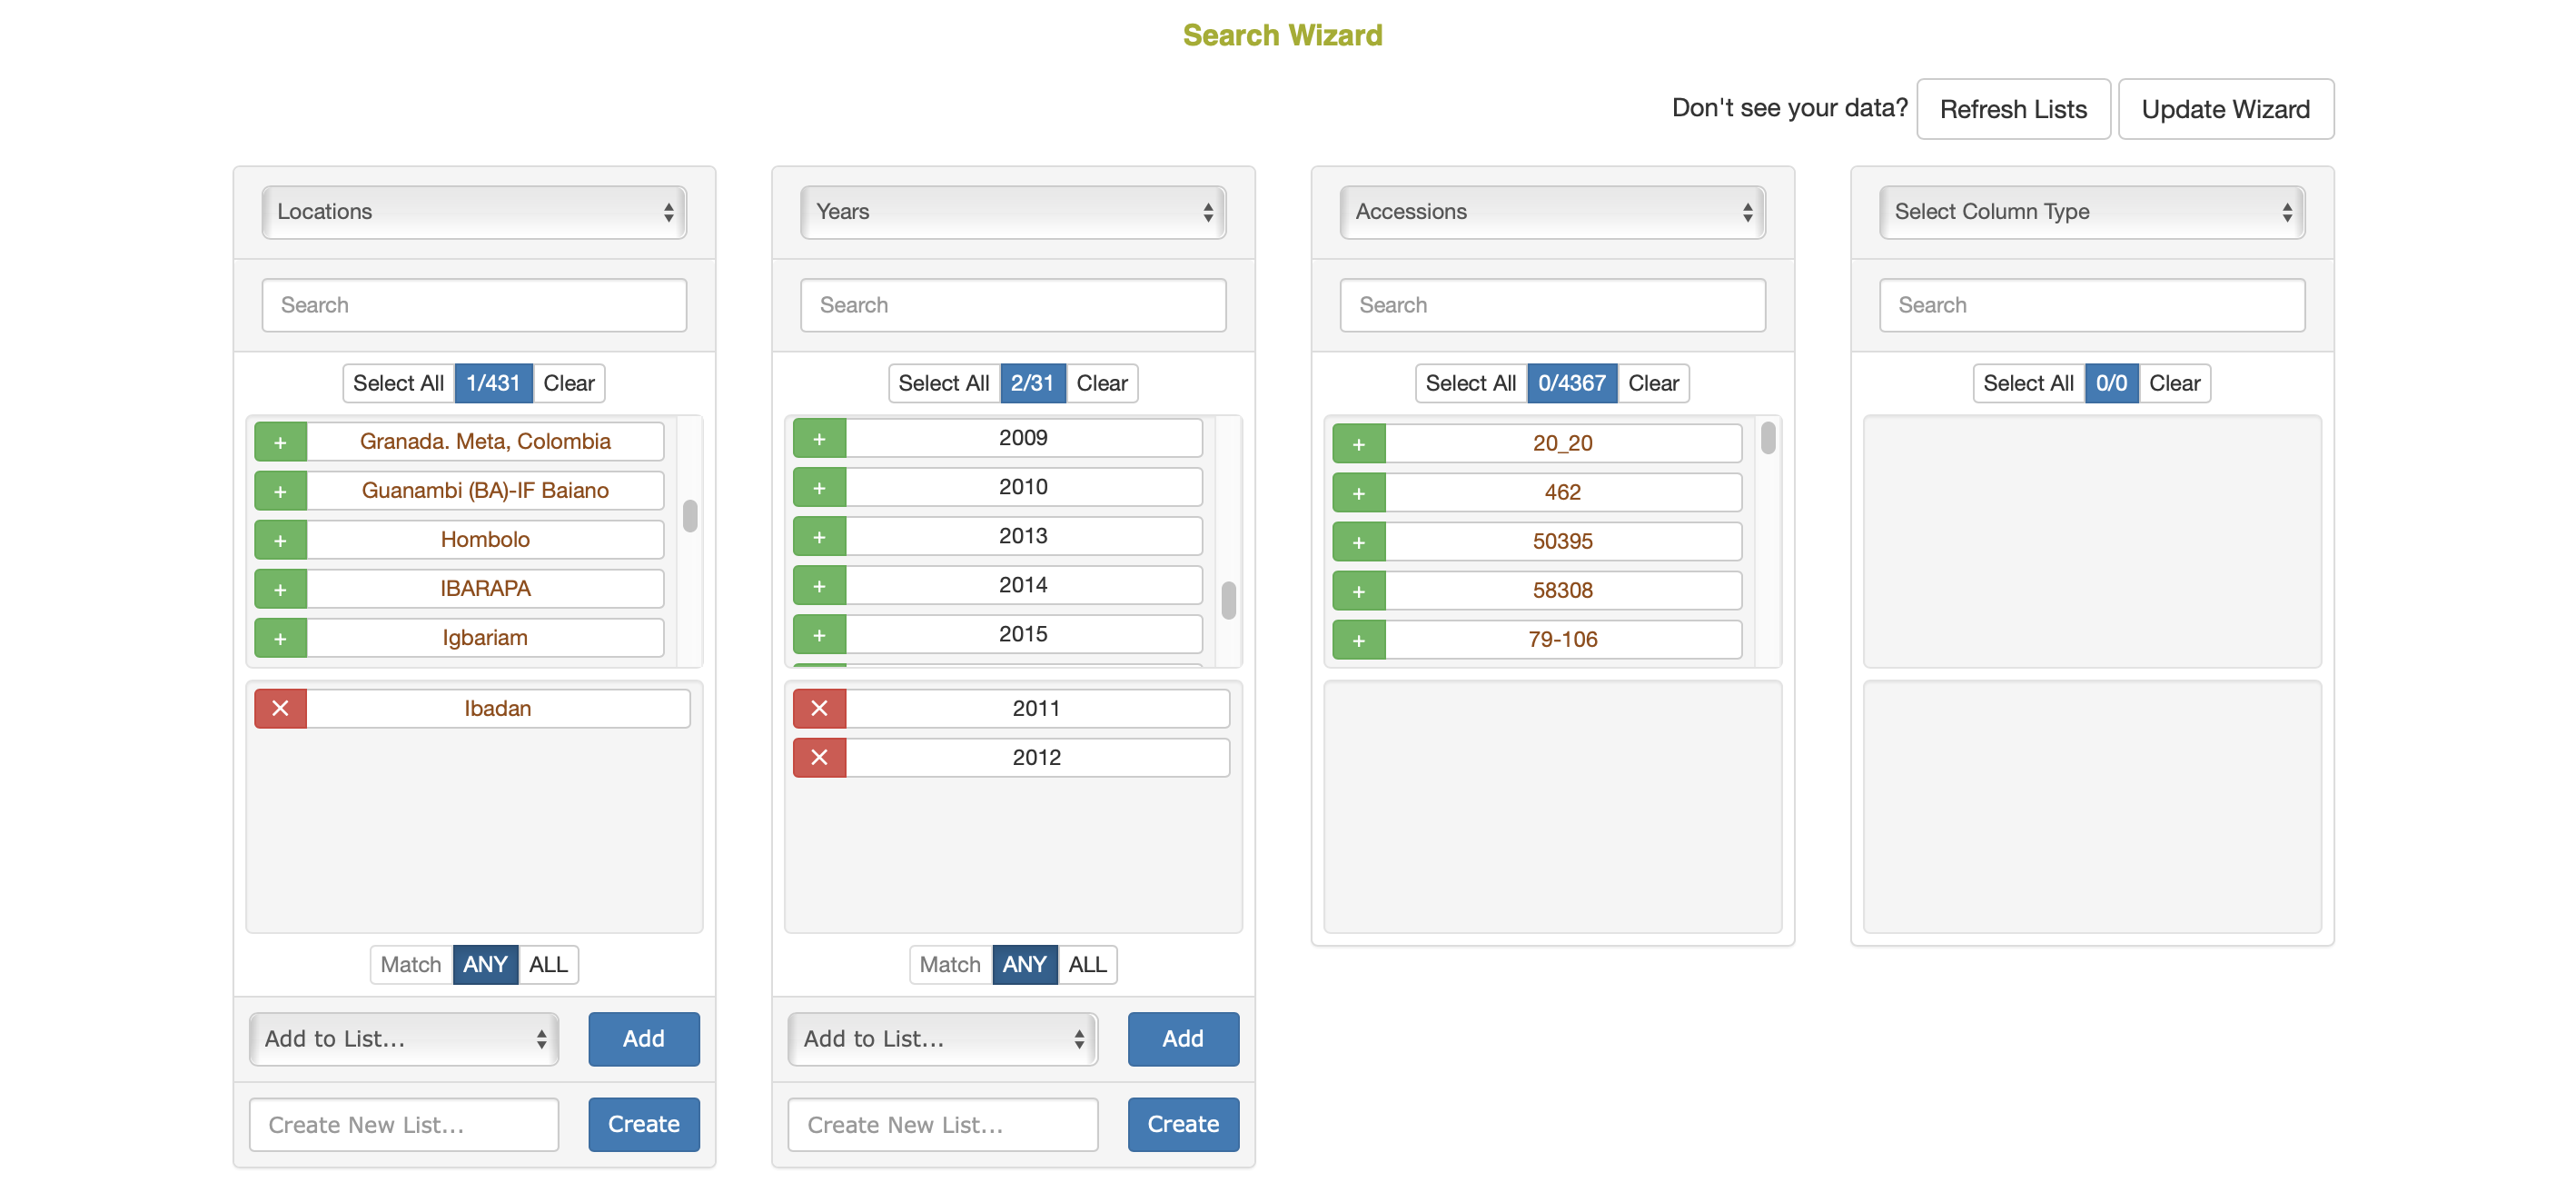
\includegraphics[width=0.95\linewidth]{assets/images/wizard_interface_selections} \end{center}

\begin{itemize}
\item
  In the example above, the ``locations'' category was chosen in the first dropdown. The first select box then displayed all the possible locations in the database. The option Ibadan was selected.
\item
  This activated the second dropdown. The category ``years'' was chosen in the second dropdown. The second select box then displayed all the years that are linked in the database to the location Ibadan. From that list, the options 2011 and 2012 were selected.
\item
  This activated the third dropdown. A final category, ``accessions'', was chosen in the third dropdown. The third select box was then populated with the 3847 accessions in the database that are linked with the location Ibadan in the years 2011 or 2012.
\end{itemize}

In addition to the basic search operations demonstrated above, users can take advantage of two more features:

\textbf{Load Selection from List}

\begin{center}
\includegraphics[width=0.25\linewidth]{assets/images/wizard_select_list} \end{center}

\begin{itemize}
\tightlist
\item
  Instead of picking a category in the first dropdown, users can instead populate the first selectbox from a list by scrolling down in the first dropdown to the ``Load Selection from List'' subheading and selecting a list. This is useful for starting queries with a list of plots, as this category is not among the options in the first dropdown.
\end{itemize}

\textbf{ANY/MIN/ALL} Toggle

\begin{center}
\includegraphics[width=0.25\linewidth]{assets/images/wizard_any_min_all_toggle} \end{center}

\begin{itemize}
\item
  By default, the search wizard combines options within a category using an OR query. In the example above, in the third panel the wizard retrieved accessions associated with the location `Ibadan' in \textbf{ANY} of the years ``2011 \textbf{OR} 2012''
\item
  If the user clicked the toggle below the second select box to change it to \textbf{ALL} before choosing accessions in the third dropdown, the wizard would instead retrieve accessions associated with the location `Ibadan' in the years ``2011 \textbf{AND} 2012''. This will be a smaller set of accessions, because any accessions used only in 2011, or only in 2012 will be excluded.
\item
  A more advanced search could use the \textbf{MIN} toggle option. This allows the user to make a query in between an ANY or ALL query, where a minimum number of matches from the selected column will be used as a filter for the next column. The minimum can be provided as either a percentage (\%) or an actual count of items (\#). In the example above, if the years 2011, 2012, and 2013 were selected in the second column, the user could enter `2' in as the minimum and select `\#' as the minimum match type. This would select accessions in the third column that were used in 2 or more of the selected years.
\end{itemize}

\begin{center}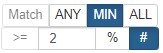
\includegraphics[width=0.25\linewidth]{assets/images/wizard_any_min_all_toggle_min_details} \end{center}

\hypertarget{how-to-use-retrieved-data}{%
\subsection{How to use retrieved data}\label{how-to-use-retrieved-data}}

\hypertarget{getting-more-info}{%
\subsubsection*{Getting more Info}\label{getting-more-info}}


Any option in the wizard select boxes (except for years) can be clicked to open a page with more details. The new page is opened in a new tab.

\hypertarget{saving-to-a-list}{%
\subsubsection*{Saving to a list}\label{saving-to-a-list}}


You can store the highlighted items in any selected box to lists. This is done using the inputs and buttons directly below the select box. \textbf{Don't forget, you must be logged in to work with lists!}

\begin{center}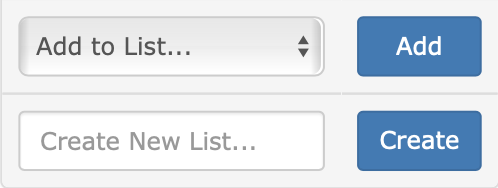
\includegraphics[width=0.5\linewidth]{assets/images/add_create_list} \end{center}

\begin{itemize}
\item
  To \textbf{add items to an existing list}, first pick an existing list using the ``Add to List\ldots{}'' dropdown on the left. Then click the ``Add'' button. A popup window will confirm the action, and display the number of items added to your existing list.
\item
  To \textbf{store items to a new list}, first type a new list name in the ``Create New List\ldots{}'' text input on the left. Then click on the ``Create'' button. A popup window will confirm the action, and display the number of items added to your new list.
\end{itemize}

\hypertarget{downloading-data}{%
\subsubsection*{Downloading Data}\label{downloading-data}}


You can download trial metadata, phenotypes and genotypes associated with the highlighted items in the wizard select boxes. This is done using the buttons in the download section at the bottom of the page. \textbf{Don't forget, you must be logged in to download data!}

\begin{center}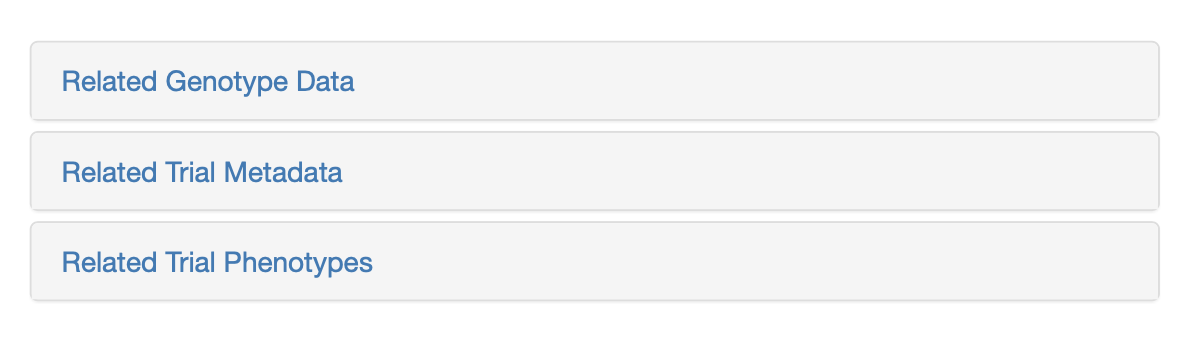
\includegraphics[width=0.75\linewidth]{assets/images/wizard_download_options} \end{center}

\hypertarget{metadata}{%
\paragraph*{Metadata}\label{metadata}}
\addcontentsline{toc}{paragraph}{Metadata}

Trial metadata can be downloaded by selecting a subset of trials from the database or based on your search categories. To download, click on ``Related Trial Metadata'', a dialog will appear. Select download format and click the ``Metadata'' button to complete your download.

\begin{center}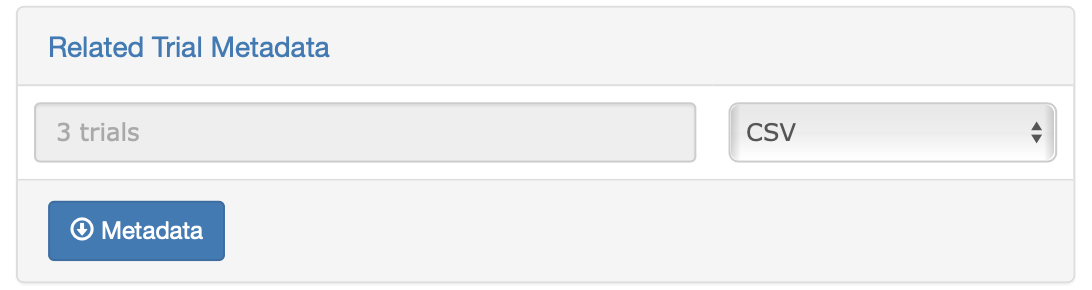
\includegraphics[width=0.75\linewidth]{assets/images/wizard_related_metadata_download} \end{center}

\hypertarget{phenotypes}{%
\paragraph*{Phenotypes}\label{phenotypes}}
\addcontentsline{toc}{paragraph}{Phenotypes}

The phenotypes download is quite flexible, and can download a subset of all the trial data in the database based on whichever categories and options you currently have selected. Simply click on the ``Related Trial Phenotypes'' link, review the options, changing or adding any additional parameters you like, then click `Download Phenotypes'.

\begin{center}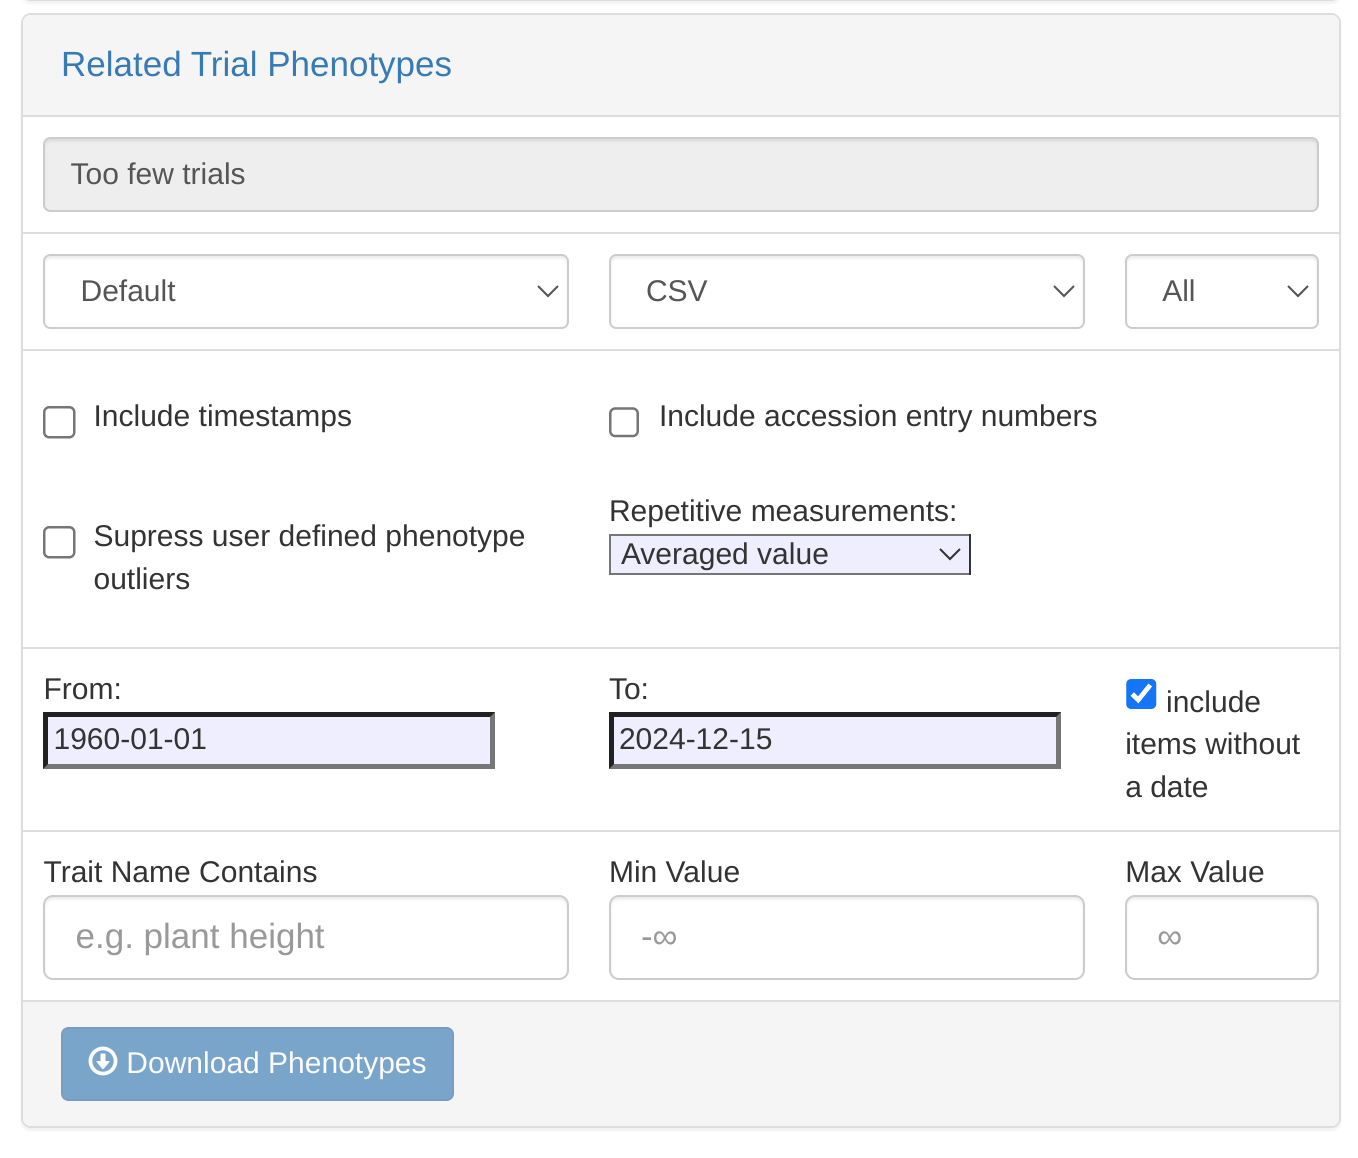
\includegraphics[width=0.75\linewidth]{assets/images/wizard_related_phenotypes_download} \end{center}

\hypertarget{genotypes}{%
\paragraph*{Genotypes}\label{genotypes}}
\addcontentsline{toc}{paragraph}{Genotypes}

The genotype download is more stringent. It requires a minimum of one accession and one genotyping protocol to be selected in the wizard select boxes. The text box in the download section of the page will help track what has been selected. Once clicked, the ``Download Genotypes'' button will download a genotype file for the selected accessions.

\hypertarget{saving-the-wizard-selections}{%
\subsubsection*{Saving the wizard selections}\label{saving-the-wizard-selections}}


As discussed above, the selections of the individual select boxes in the wizard can be saved separately to a list. The lists can be used as inputs in other tools on the site. However, sometimes creating a selection is quite time consuming and restoring the selections from four different lists would be cumbersome too. Therefore, the selections can be saved together in a dataset, and named for later retrieval. This is done in the section ``Load/Create Datasets'' that is below the first two wizard select boxes. To select an existing dataset, one uses the ``Load Dataset'' dropdown. A particular dataset can be chosen, and the ``Load'' button can be clicked to retrieve and display the dataset in the wizard. To create a new dataset using items that are selected in the wizard, one can enter the name of the new dataset in the ``Create New Dataset'' text box. Once the dataset has been given a name, clicking the ``Create'' button will save the new dataset.

\begin{center}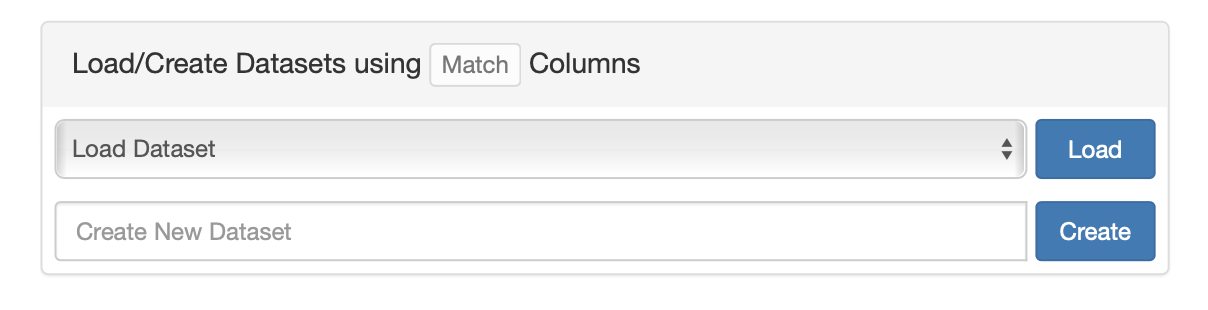
\includegraphics[width=0.75\linewidth]{assets/images/wizard_load_create_dataset} \end{center}

\hypertarget{updating-the-wizard}{%
\subsection{Updating the Wizard}\label{updating-the-wizard}}

The search wizard uses a copy of the database, or a cache, to return results quickly. If data appears to be missing, it usually means that the cache needs to be updated. Users with submitter privileges or above can do this using the `Update Wizard' button. One can also use the `Refresh Lists' button to update the available lists.

\begin{center}
\includegraphics[width=0.75\linewidth]{assets/images/wizard_update_list_refresh} \end{center}

This will take just a few seconds in small databases, but may take a few hours to complete in larger databases.

\hypertarget{accessions-and-plot-search}{%
\section{Accessions and Plot Search}\label{accessions-and-plot-search}}

Accessions and their related materials (cross, plant, plot, population, tissue\_sample, training population) can be searched by using ``Search Accessions and Plots'' page. On this page, ``accession'' is the default stock type; however, you can change stock type by selecting an option from the drop-down list. From this page you can construct detailed queries for stock types. For example, by using the ``Usage'' section, the ``Properties'' section, and the ``Phenotypes'' section you could search for accessions which were diploids used in a specific year and location and were also phenotyped for height. You can also search for accessions based on genetic properties, such as the location of an introgression on a specific chromosome.

\begin{center}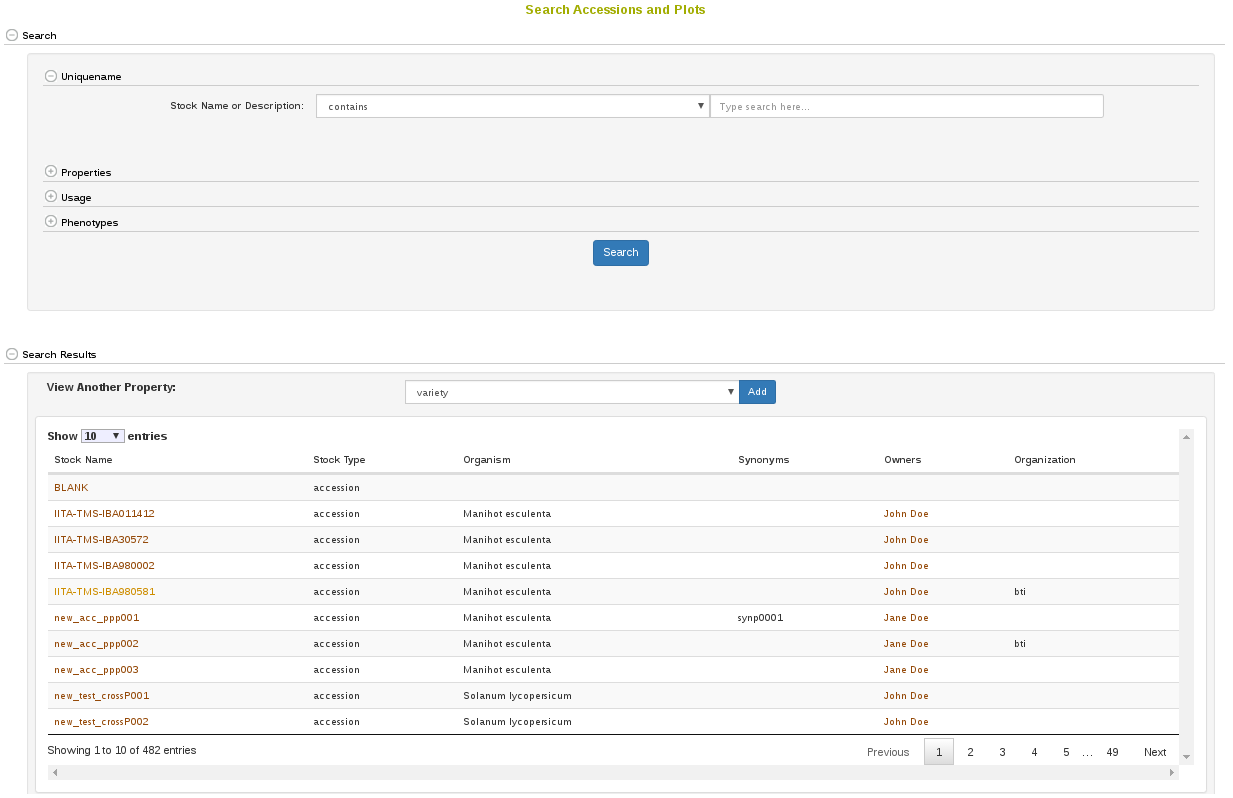
\includegraphics[width=0.95\linewidth]{assets/images/search_accessions} \end{center}

It is possible to query over any of the available properties, such as ``ploidy\_level'', ``country of origin'', ``introgression\_chromosome'', etc.

\begin{center}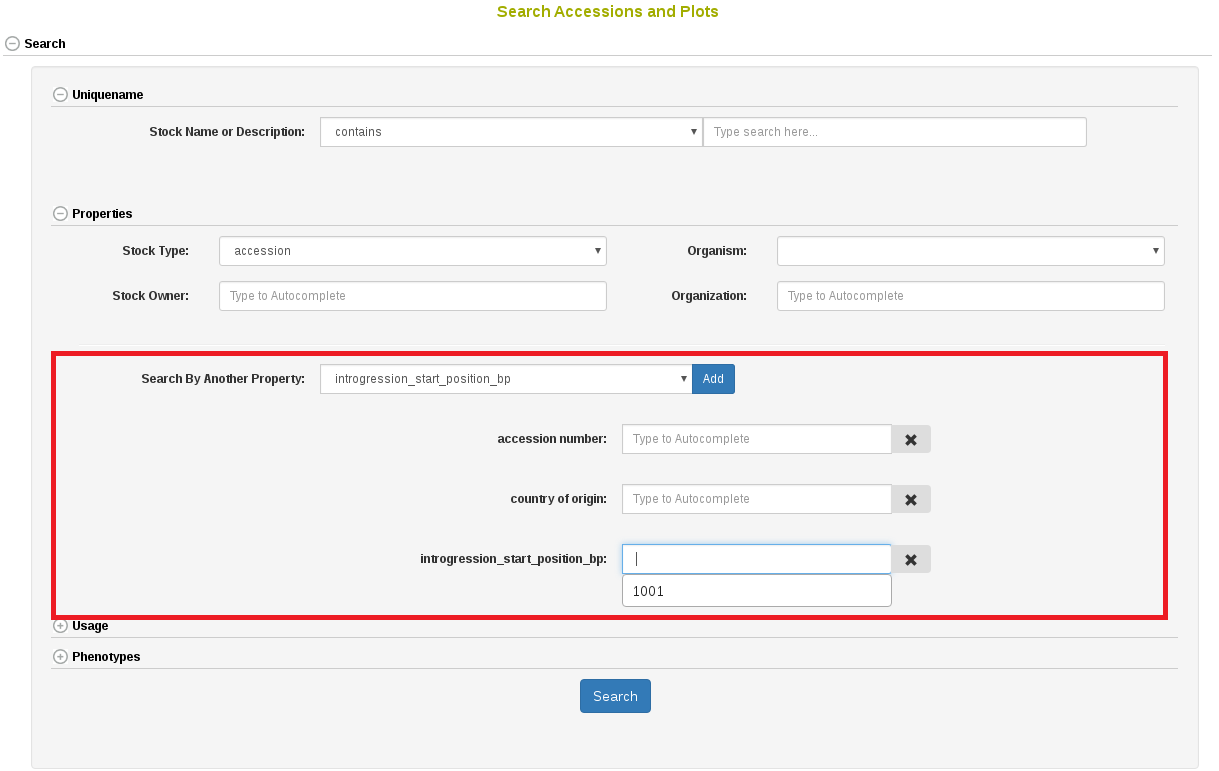
\includegraphics[width=0.95\linewidth]{assets/images/search_accessions_properties_search} \end{center}

In the search result table it is possible to select any of the available properties to view.

\begin{center}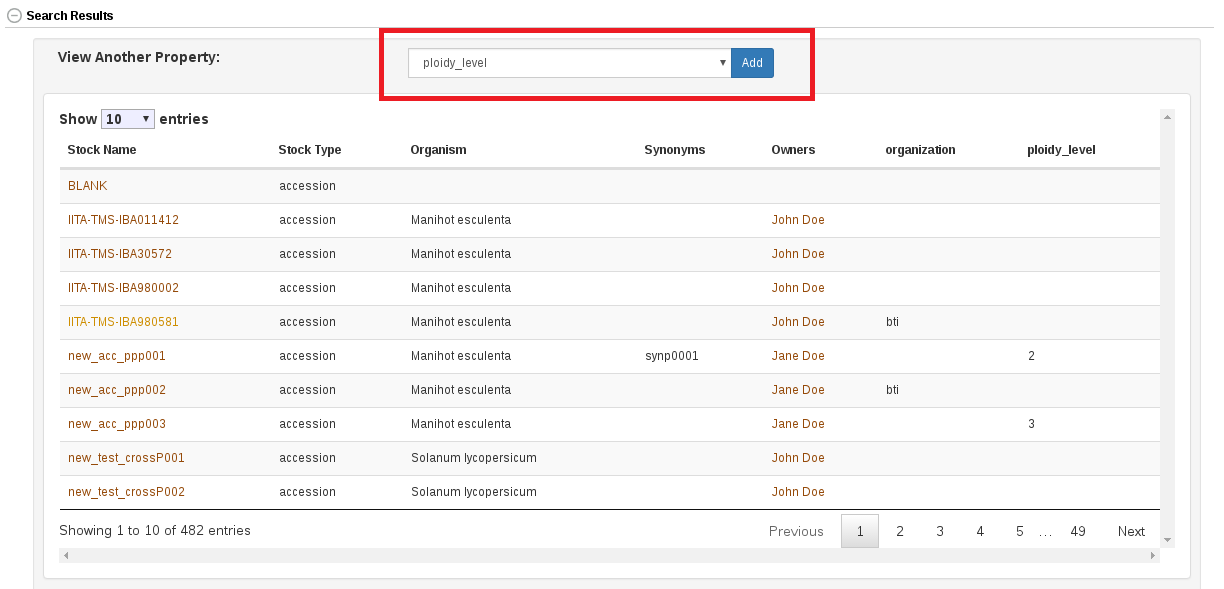
\includegraphics[width=0.95\linewidth]{assets/images/search_accessions_properties_view} \end{center}

At the bottom of the accession search there is a phenotype graphical filtering tool. Here you can filter down accessions based on combinations of trait performance. The filtered down accessions are then able to be saved to a list.

\begin{center}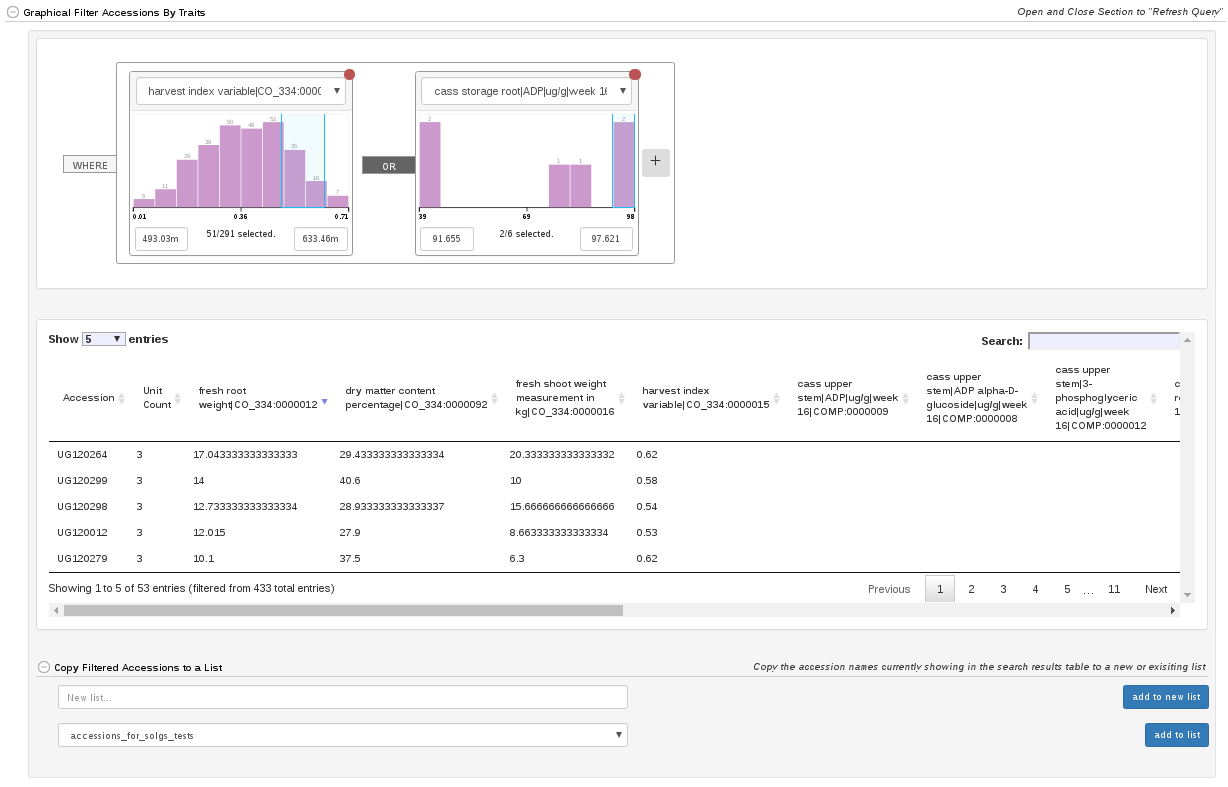
\includegraphics[width=0.95\linewidth]{assets/images/search_accessions_graphical_filtering} \end{center}

For information on adding Accessions please see the Managing Accessions help. For information on how field trial plots, plants, tissue samples, and subplots are added to the database, please see the Managing Field Trials help.

\hypertarget{trials-search}{%
\section{Trials Search}\label{trials-search}}

Trials on the database can be searched based on trial name, description, breeding program, year, location, trial type, design, planting date, and harvest date.

\begin{center}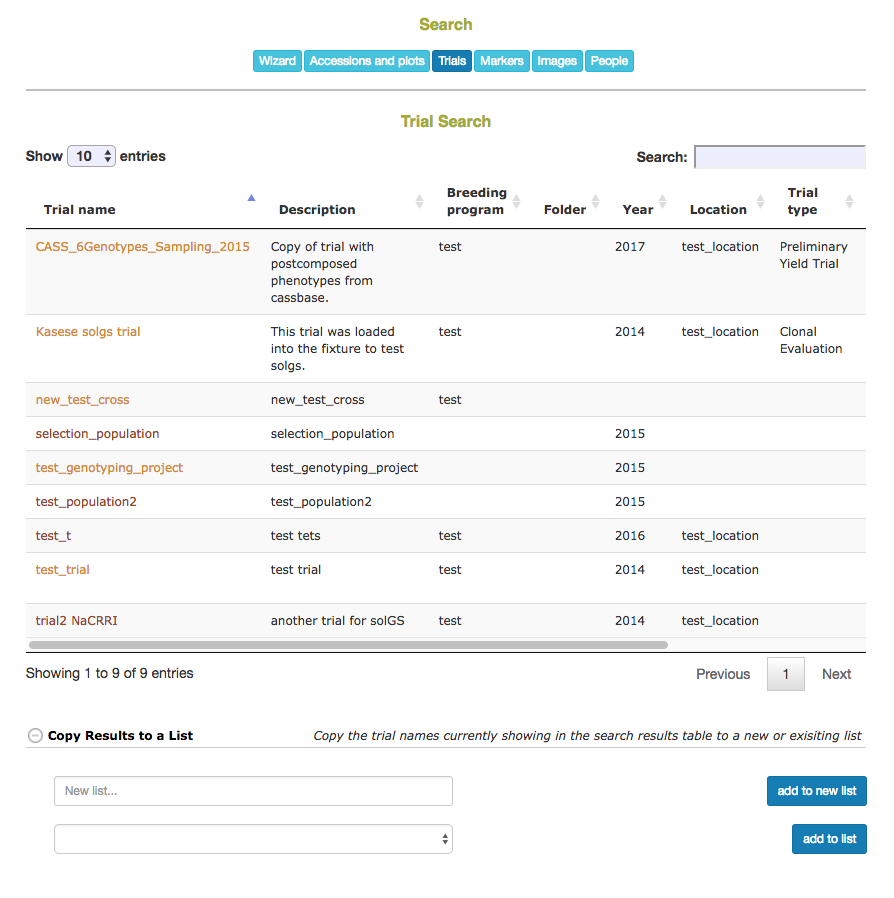
\includegraphics[width=0.95\linewidth]{assets/images/trial_search} \end{center}

\hypertarget{trait-search}{%
\section{Trait Search}\label{trait-search}}

On the Trait Search page (menu item \texttt{Search\ \textgreater{}\ Traits}), traits in the database can be searched by ID, name, or descripiton. Optionally, a starting list of traits can be selected to filter down results.

\begin{center}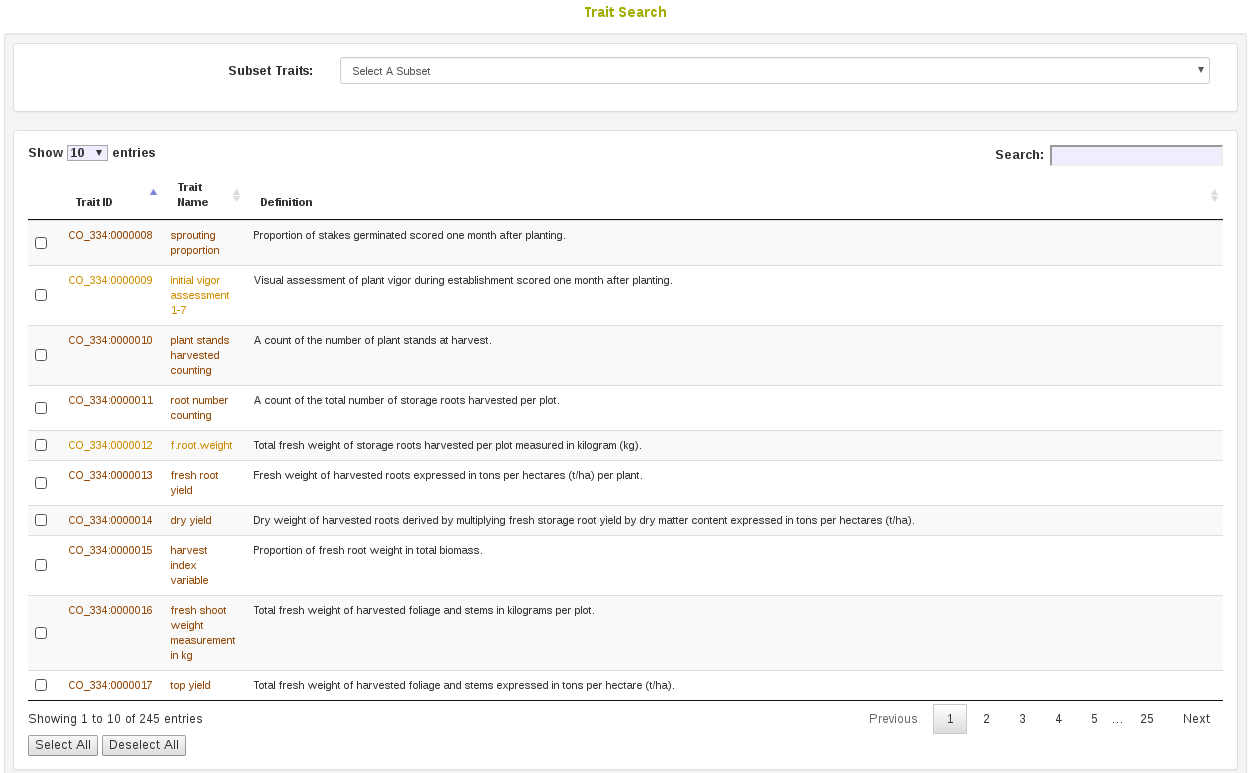
\includegraphics[width=0.95\linewidth]{assets/images/trait-search-default} \end{center}

Selecting traits in the results of the search allows one to add the selected results to a trait list, or create a new trait list from the select results.

\begin{center}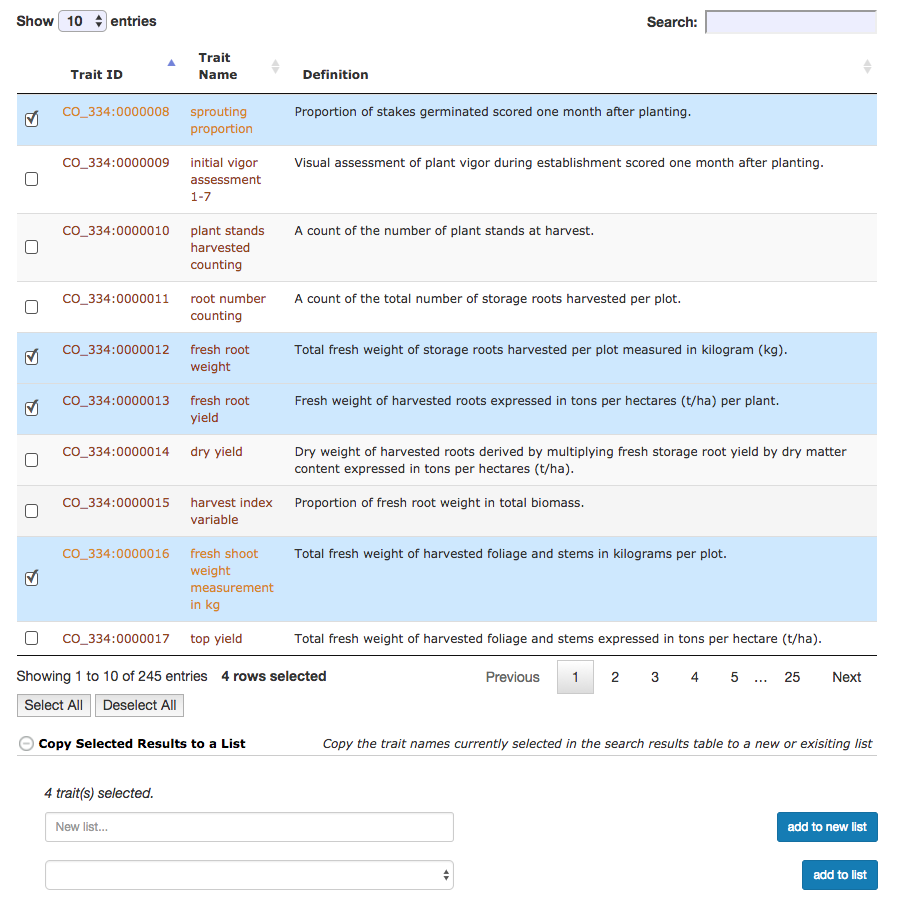
\includegraphics[width=0.95\linewidth]{assets/images/trait-search} \end{center}

\hypertarget{ontology-browser}{%
\section{Ontology Browser}\label{ontology-browser}}

A more advanced tool for searching for Traits is the ontology browser, available by clicking on Analyze and Ontology Browser. From here you can search ontologies and see the various classifications of terms in a tree display.

\begin{center}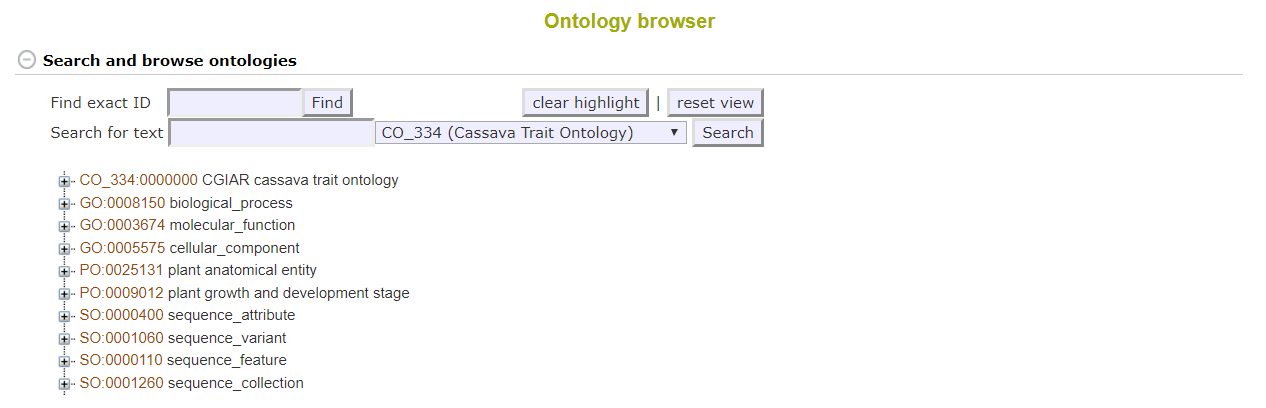
\includegraphics[width=0.95\linewidth]{assets/images/ontology_browser} \end{center}

The terms which appear in the Trait Search in 2.4 are only variable terms. The ontology browser shows these variables as different from their grouping terms by indicating VARIABLE\_OF like in the following screenshot.

\begin{center}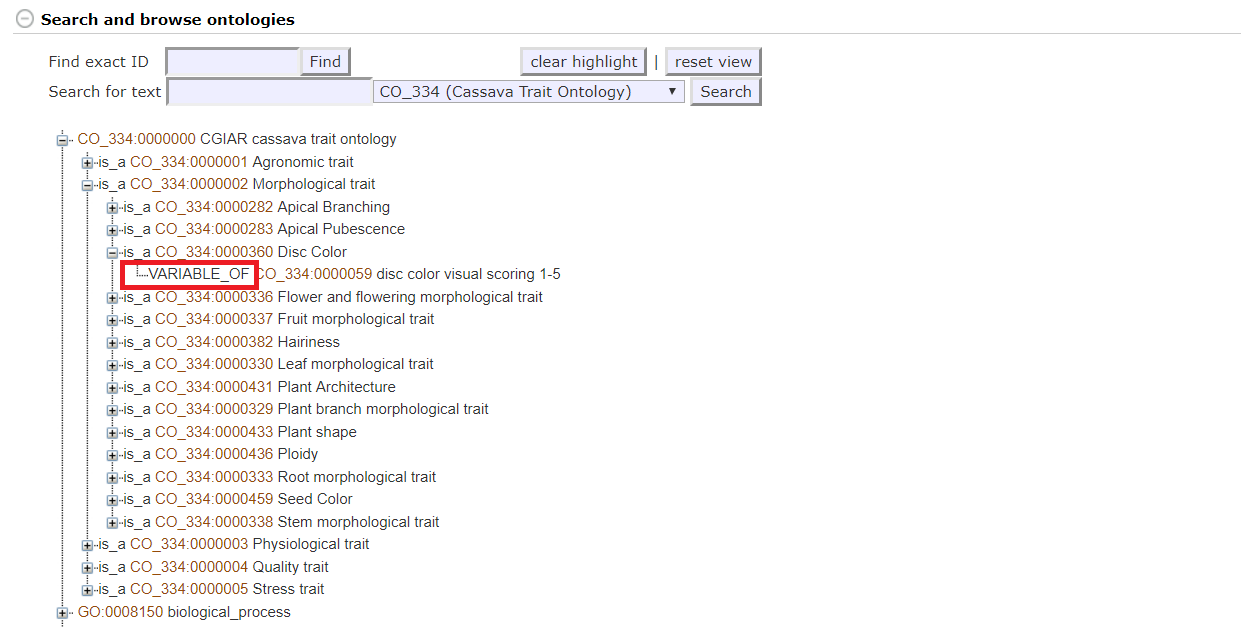
\includegraphics[width=0.95\linewidth]{assets/images/ontology_browser_variable} \end{center}

\hypertarget{search-seedlots}{%
\section{Search Seedlots}\label{search-seedlots}}

Seedlots are different from Accessions in that they represent the physical seed being evaluated in an experiment. Seedlots have things like physical storage locations and seed quantities, which accessions do not. To search for available seedlots you go to Manage and then click Seed Lots. By clicking Search Seedlots, you can specify query information. The results from your search will be in the table below the search form.

\begin{center}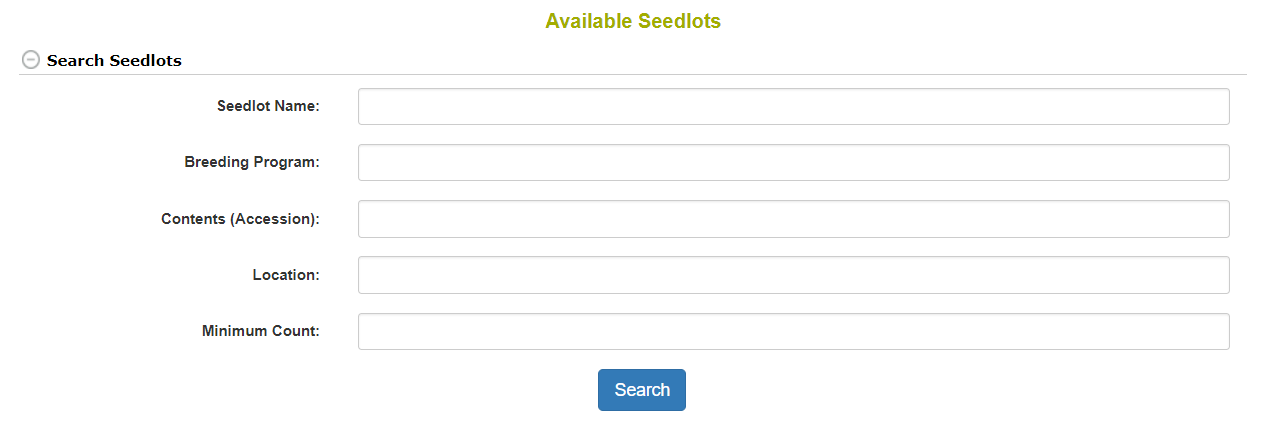
\includegraphics[width=0.95\linewidth]{assets/images/search_seedlots} \end{center}

\begin{center}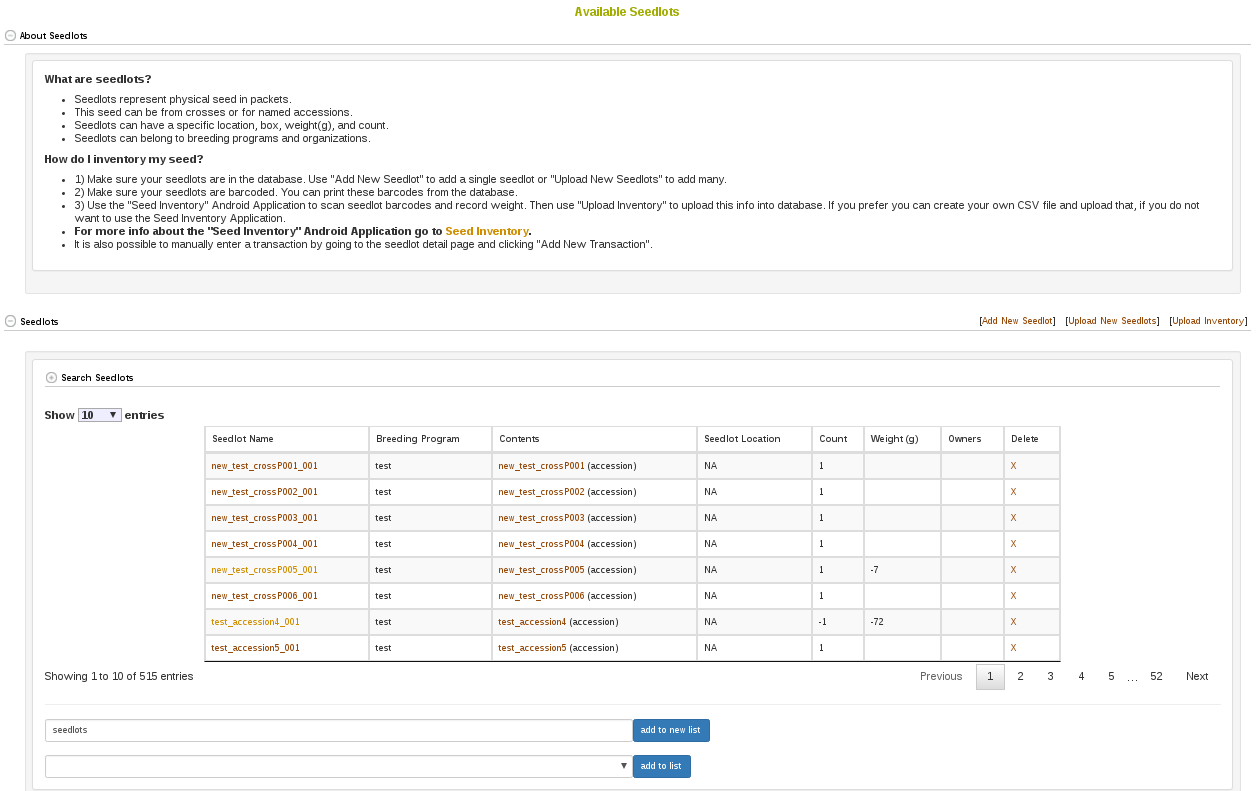
\includegraphics[width=0.95\linewidth]{assets/images/manage_seedlots} \end{center}

\hypertarget{managing-user-roles}{%
\chapter{Managing User Roles}\label{managing-user-roles}}

\begin{center}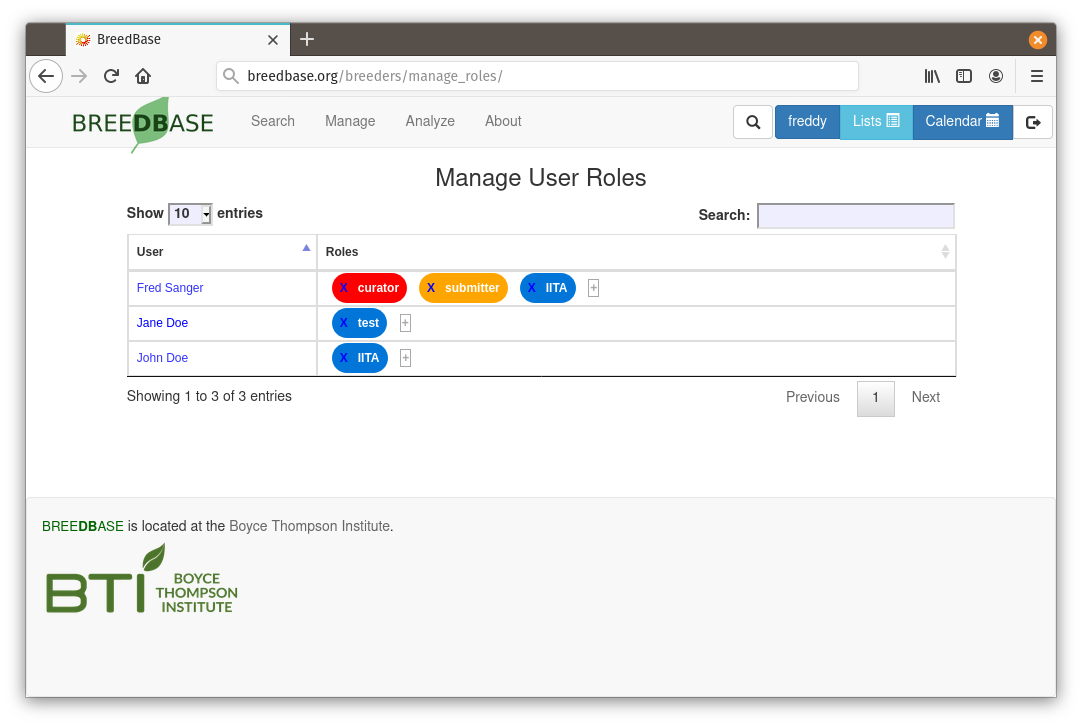
\includegraphics[width=0.95\linewidth]{assets/images/manage_user_roles_page} \end{center}

\hypertarget{what-are-user-roles}{%
\section{What are User Roles?}\label{what-are-user-roles}}

Every user account in Breedbase has one or more associated ``roles'' that determine the authorizations (what the user is allowed to do) in the database. There are three fundamental roles, ``curator'', ``submitter'', and ``user'', which determine basic read/write levels. The ``curator'' status can read and write everything in the database. The ``submitter'' status can add information and edit or delete previously submitted information. The ``user'' type can only read data. Additional roles represent the breeding programs, and are sometimes used to fine-tune write and edit capabilities, as it necessary for multiple users in a breeding program to edit each other's data.

\hypertarget{the-manage-user-roles-page}{%
\section{The Manage User Roles page}\label{the-manage-user-roles-page}}

In the ``Manage'' menu, select the item ``User Roles''. This will show the current users in the database with their associated roles. If you are logged in as a curator, the table will show system roles as well as breeding program roles; if you are logged in as a submitter or user, it will show breeding program membership.

If logged in as a ``curator'', the roles can be added or deleted.

\begin{itemize}
\tightlist
\item
  To delete a role, click on the X in the role name. A confirm dialog will be displayed to prevent accidental deletion.
\item
  To add a role, click on the plus sign next to the roles. A dialog will pop up with a list of roles. Select the desired role and click ``Submit''.
\item
  The new role should be displayed next to the user immediately.
\item
  Role deletions and additions will be effective immediately.
\end{itemize}

It is recommended that few users be given the ``curator'' privileges to avoid confusion over data ownership and accidental data overwriting and deletion.

\hypertarget{managing-breeding-programs}{%
\chapter{Managing Breeding Programs}\label{managing-breeding-programs}}

New breeding programs can be added by using ``Add New Program'' button on the ``Manage Breeding Programs'' page.

\begin{center}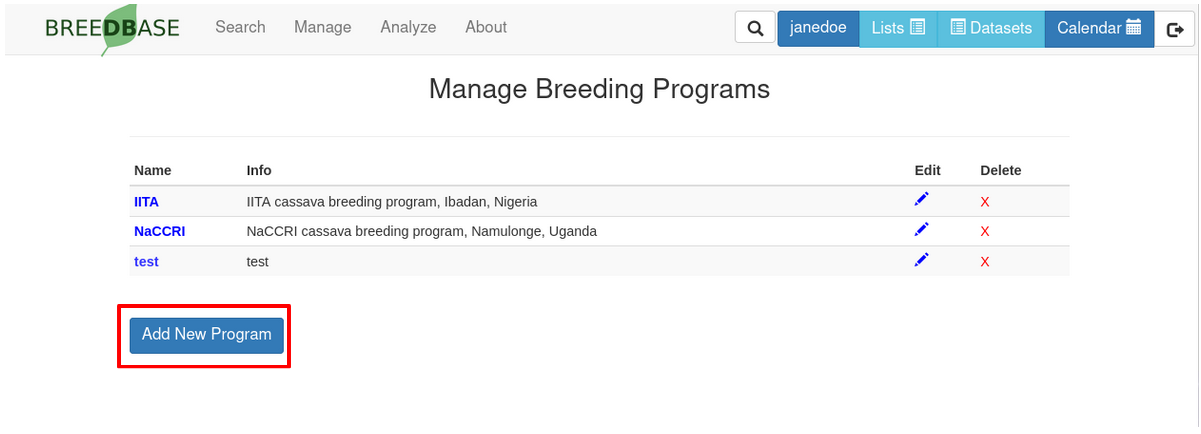
\includegraphics[width=0.95\linewidth]{assets/images/breeding_programs_screenshot} \end{center}

Clicking on the ``Add New Program'' button will generate a blank form for you to fill out the name and description of the breeding program that you want to add. After completing the form, click on ``Add Breeding Program'' button to finish the process.

\begin{center}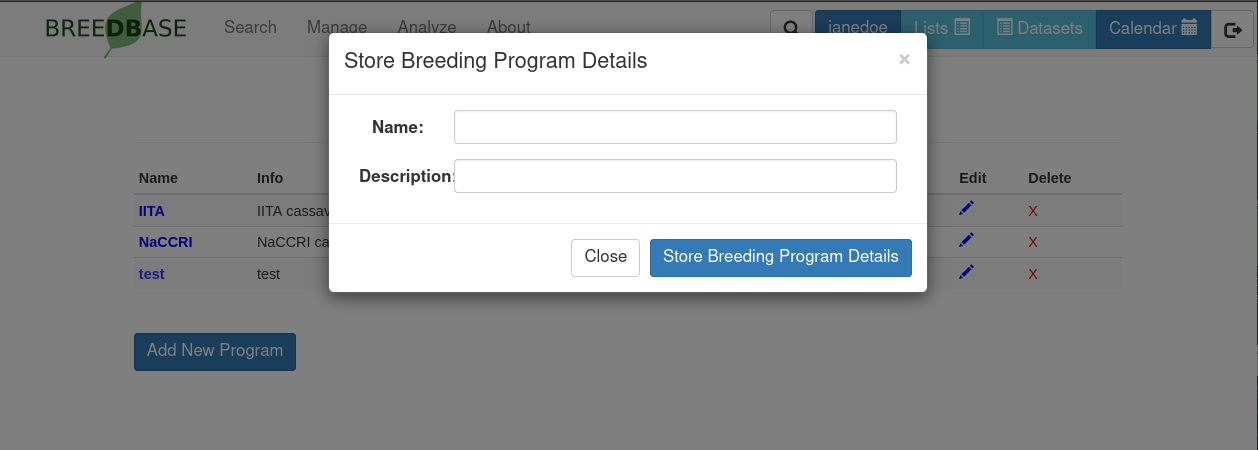
\includegraphics[width=0.95\linewidth]{assets/images/new_program_screenshot} \end{center}

\hypertarget{managing-locations}{%
\chapter{Managing Locations}\label{managing-locations}}

Field locations can be managed using the ``\textbf{Manage Locations}'' page. On this page, locations in the database are organized based on their breeding programs. Each location has a link to trials conducted in that location. To add a new location, click on the ``Upload New Locations'' button that links to the ``Upload Locations'' form.

\begin{center}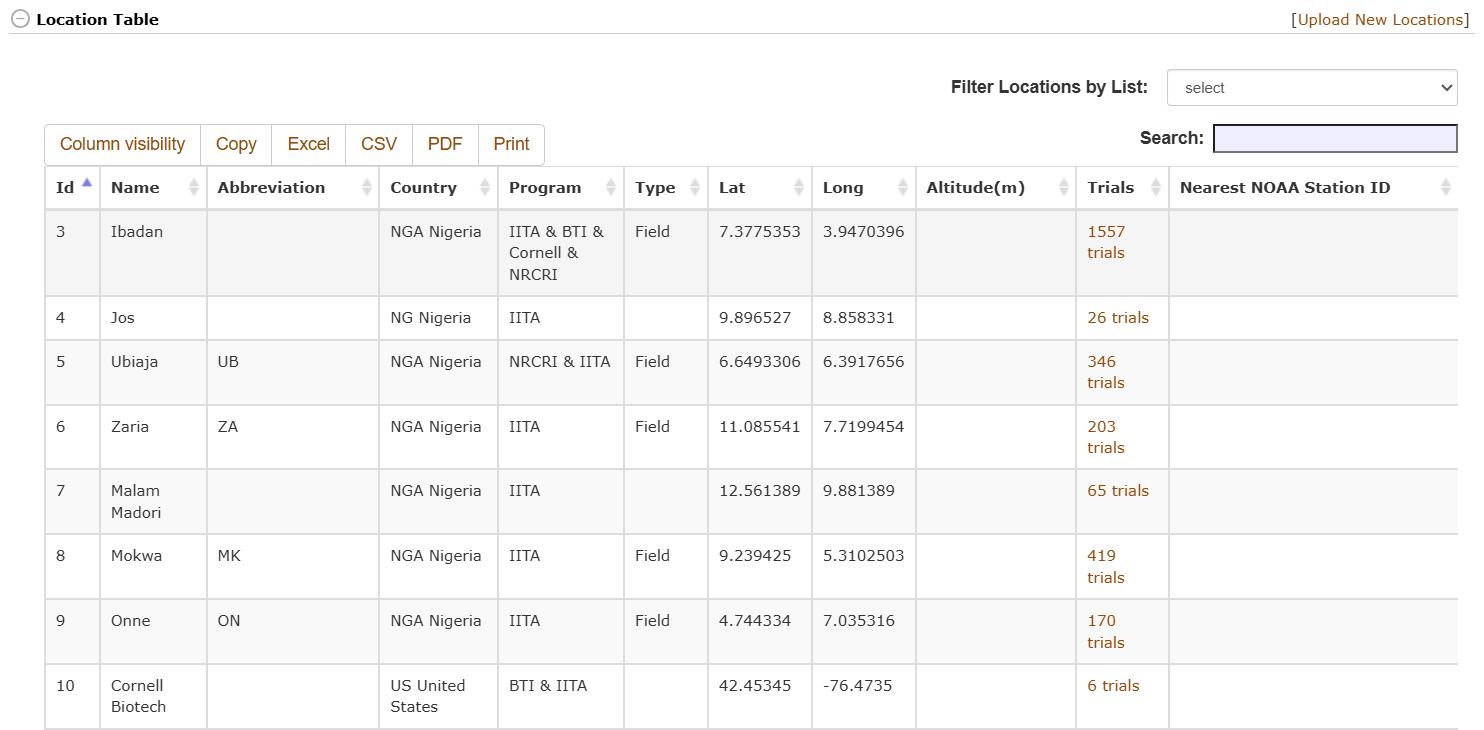
\includegraphics[width=0.95\linewidth]{assets/images/image141} \end{center}

The ``Upload Locations'' describes how to build a spreadsheet with location data for upload. Name, abbreviation, country code, country name, program, type, latitute, longitude, and elevation are all required. The NOAA station ID is optional. Link a spreadhsheet to the form and click ``Upload'' to add those locations to the database.

\begin{center}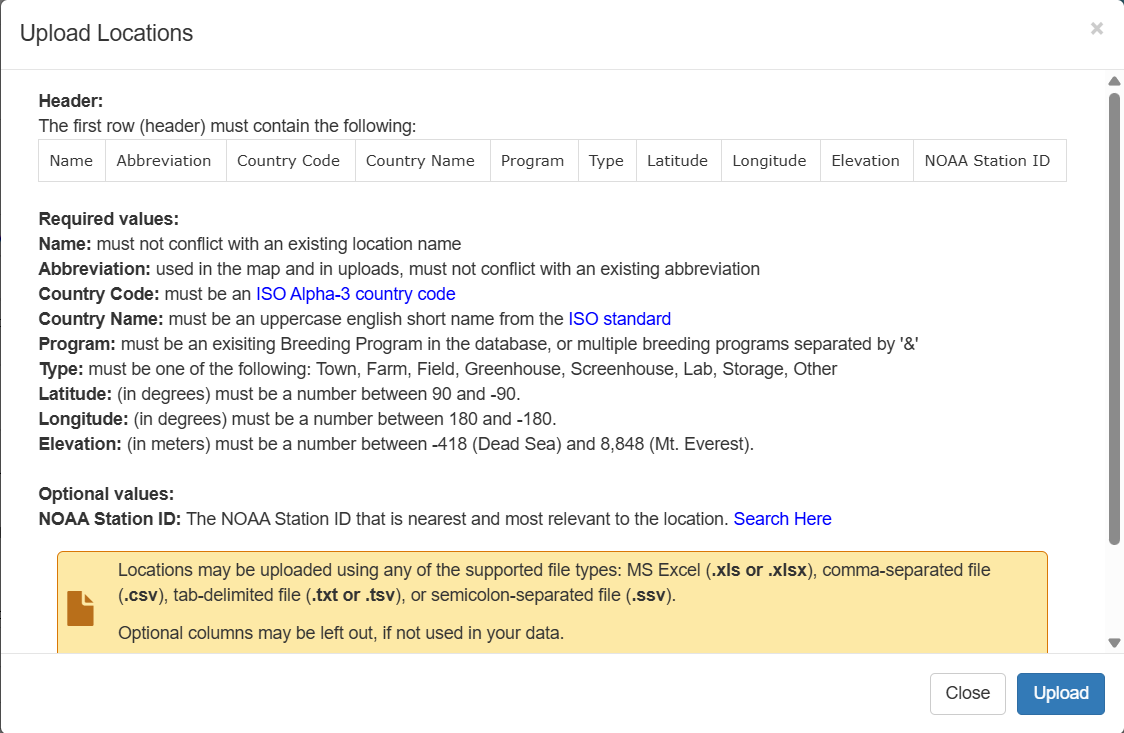
\includegraphics[width=0.95\linewidth]{assets/images/image187} \end{center}

Alternatively, locations can be viewed and added via the map. Hover over an icon on the map to see the location details and trials linked to that location. Click on the map to open the new location dialog. Fill in the same information that would be used in the spreadsheet upload to add a new location.

\begin{center}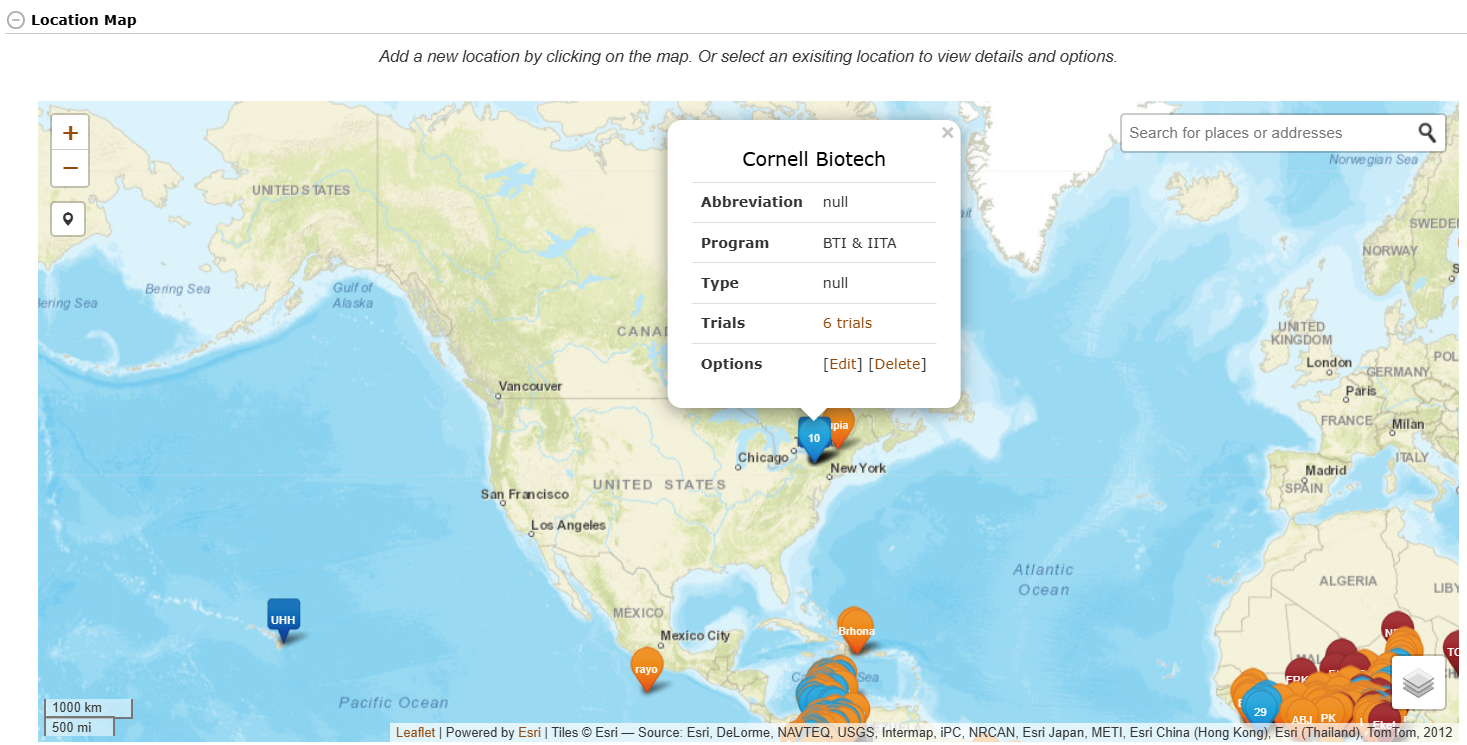
\includegraphics[width=0.95\linewidth]{assets/images/location_map} \end{center}

\hypertarget{managing-accessions}{%
\chapter{Managing Accessions}\label{managing-accessions}}

The ``Manage Accession'' page provides links for adding new accessions. New accessions can be added to the database by either using a List or by uploading an Excel file (either XLS or XLSX format). Both options are explained in more detail below. To begin, click on the ``Add Accessions or Upload Accession Info'' link.

\begin{center}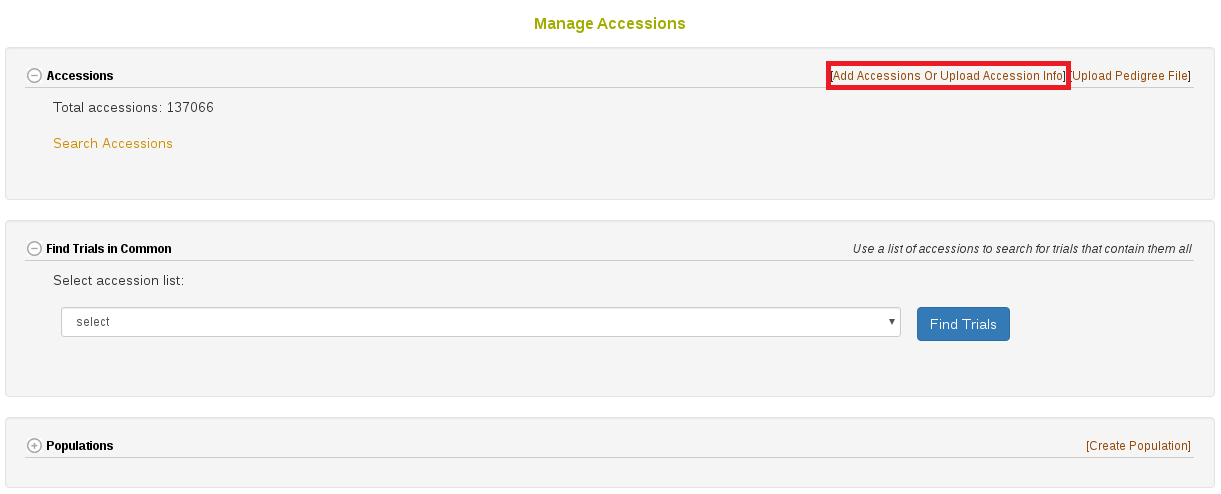
\includegraphics[width=0.95\linewidth]{assets/images/manage_accessions_add_accessions_link} \end{center}

This will open a dialog allowing you to select either ``Using Lists'' or ``Uploading a File''.

\hypertarget{add-accessions-using-a-list}{%
\section{Add Accessions Using A List}\label{add-accessions-using-a-list}}

First we will show how to add accessions ``Using Lists''.

\begin{center}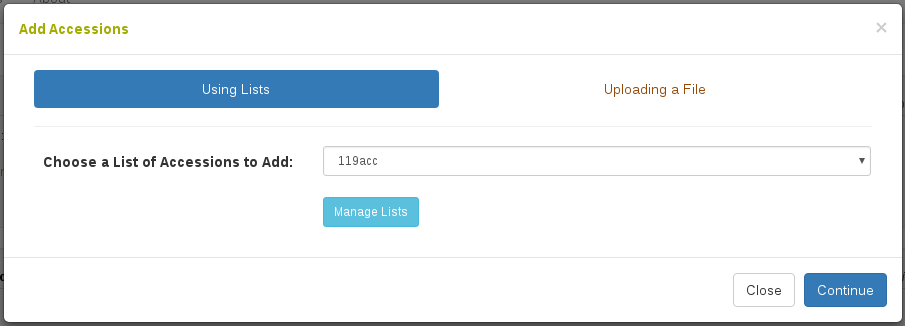
\includegraphics[width=0.95\linewidth]{assets/images/manage_accessions_add_accessions_using_lists} \end{center}

Here you select an accession list which you have previously made (see List Manager chapter). If you need to create or edit your list you can do so now by clicking ``Manage Lists''. After selecting your list, click ``Continue''.

The contents of the list will be checked against the database, and elements that are already present will be flagged. A dialog will appear that will show the accessions which already exist in the database.

\begin{center}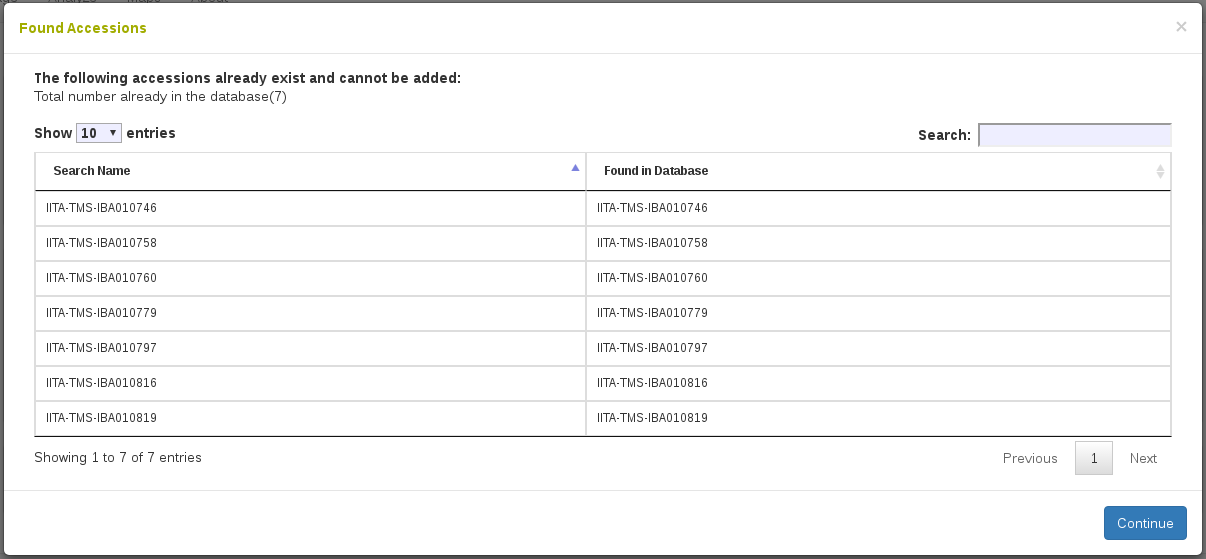
\includegraphics[width=0.95\linewidth]{assets/images/manage_accessions_add_accessions_found} \end{center}

After clicking on the ``Continue'' button, the next dialog will appear with accessions that have very similar names as the accession that you are adding. In the example below, there are two accession with very similar names to accessions already in the database. `TME0419' is very similar to `TME419', and probably represent the same line, so it would be a mistake to add this the database again. Duplicate lines in the database should be avoided, as they cause problems when evaluating lines; data is divided up among several duplicates, making it harder to get the full picture about an accession.

\begin{center}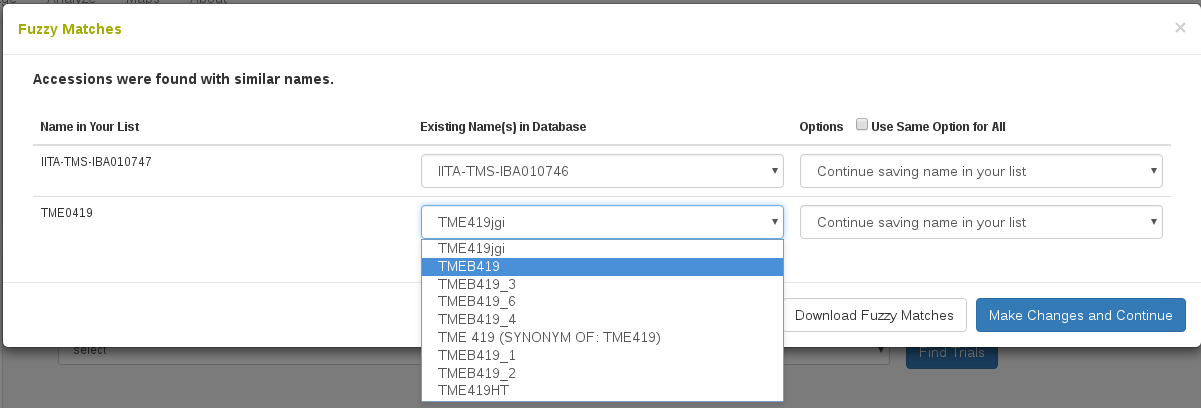
\includegraphics[width=0.95\linewidth]{assets/images/manage_accessions_add_accessions_fuzzy} \end{center}

To avoid situations in adding a mistaken duplicate accession, the database gives you options for moving forward with these very similar looking accession names. You can either ``continue saving the name in your list'', ``replace name in your list with selected existing name'', ``remove name in your list and ignore'', or ``add name in your list as a synonym to selected existing name''.

\begin{center}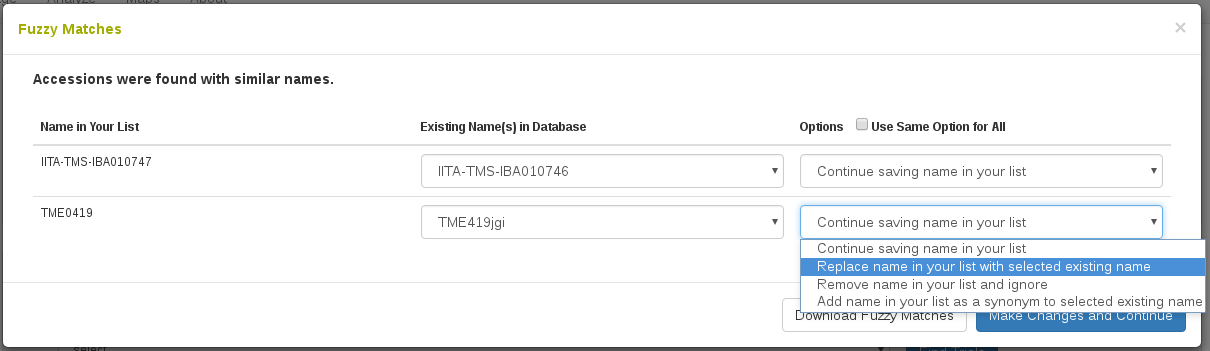
\includegraphics[width=0.95\linewidth]{assets/images/manage_accessions_add_accessions_fuzzy_options} \end{center}

Clicking ``Download Fuzzy Matches'' will return a tabular result of the ``fuzzy'' accession name results shown. Click ``Make changes and continue'' to move on.

The final dialog shows the accessions that will be added. Here you need to assign the species of these accessions. You can optionally group the accessions into a population and/or add an organization for the accessions.

\begin{center}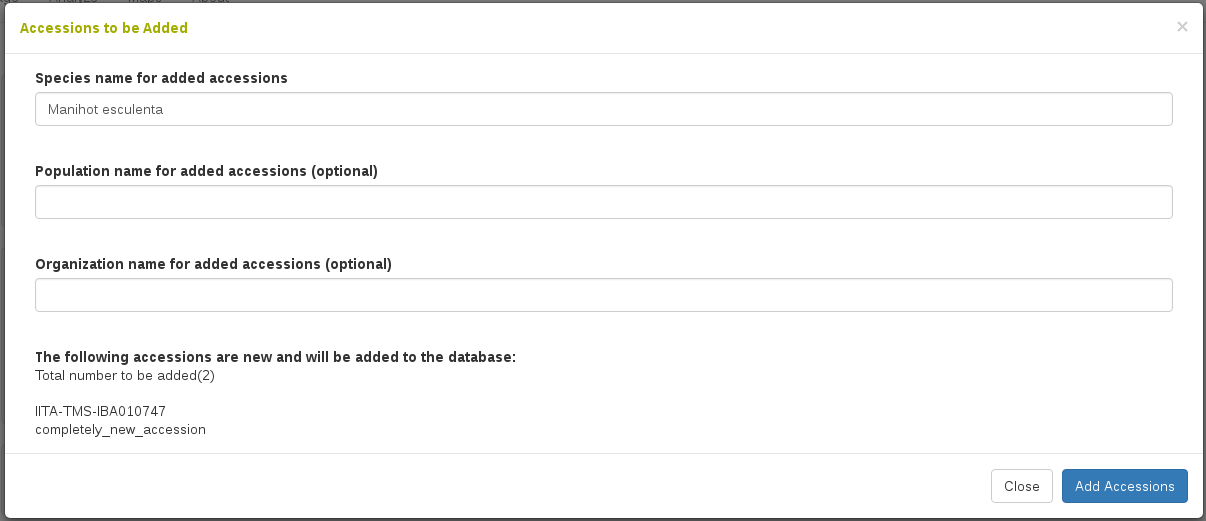
\includegraphics[width=0.95\linewidth]{assets/images/manage_accessions_add_accessions_complete_using_list} \end{center}

Once you click ``Add Accessions'', the new accessions will be created in the database and you will see the following confirmation dialog, which includes links to the newly created accessions.

\begin{center}\includegraphics[width=0.95\linewidth]{assets/images/manage_accessions_add_accessions_saved} \end{center}

\hypertarget{uploading-accessions-and-accessions-info-from-a-file}{%
\section{Uploading Accessions and Accession's Info From A File}\label{uploading-accessions-and-accessions-info-from-a-file}}

Uploading accessions using a file is very similar to using a list, but enables you to add a variety of attributes, such as synonyms or ploidy levels, to the accessions in bulk.

\begin{center}\includegraphics[width=0.95\linewidth]{assets/images/manage_accessions_add_accessions_using_file} \end{center}

Clicking on ``Spreadsheet format'' will show the required structure of the spreadsheet. The file must be XLS or XLSX format and can contain a number of header columns as attributes. It is important that you use exactly the same header column names as listed here. In columns that indicate that many attribute values can be passed at once using (s), such as synonym(s), you can pass a comma separated list of values, such as `synonym1,synonym2'.

\begin{center}\includegraphics[width=0.95\linewidth]{assets/images/manage_accessions_add_accessions_spreadsheet_info} \end{center}

Once you have selected your XLS or XLSX file for upload, click ``Continue''.

The following process is the same way as with lists:

The first dialog which can appear will show accession names which are already in the database.

Click ``Continue'' and the next dialog that can appear will show ``fuzzy'' matches for the accession names you are trying to upload. Here you can choose to prevent adding accession names which look very similar to each other as wrongly duplicated accessions.

Click ``Continue'' and the final dialog that will appear will show the information to be added into the database. Here it is divided into accession names that are new and accession names that already exist in the database; however, for the accession names that already exist it will show additional attributes that originated from your file that will be added to these accessions.

\begin{center}\includegraphics[width=0.95\linewidth]{assets/images/manage_accessions_add_accessions_complete_using_file} \end{center}

Once you click ``Add Accessions'', the new accessions and information will be created in the database and you will see the following confirmation dialog, which includes links to the created and updated accessions.

\begin{center}\includegraphics[width=0.75\linewidth]{assets/images/manage_accessions_add_accessions_saved} \end{center}

\hypertarget{email-alert-for-accession-upload}{%
\section{Email alert for accession upload}\label{email-alert-for-accession-upload}}

When uploading a large number of accessions from a file, uploads can take a while, as the system needs to perform a series of checks on each entry. You have the option to receive an email notification about the status and results of your upload by clicking the ``Email Alert'' checkbox. By default, the system will use the email address associated with your account, but you have the option of entering a different email address if you prefer. After submitting, the upload process runs in the background, allowing you to continue using the interface without interruptions. Once the process completes, you will receive an email with the upload results, including any warnings or errors that may have occurred during the upload.

\begin{center}\includegraphics[width=0.75\linewidth]{assets/images/accession_upload_using_email} \end{center}

\hypertarget{add-parentage-pedigree-information-to-accessions}{%
\section{Add Parentage (Pedigree) Information to Accessions}\label{add-parentage-pedigree-information-to-accessions}}

Pedigree data can be uploaded from your computer by clicking on ``Upload Pedigree File''

\begin{center}\includegraphics[width=0.95\linewidth]{assets/images/image286} \end{center}

You can find detailed information on how to prepare pedigree file by clicking on ``File format information''. The file format can be tab or comma delimited text file, or Excel files (.xls or .xlsx).

The currently supported format has four columns:

progeny name female parent accession male parent accession type

Type can be biparental, self, backcross, sib, polycross, reselected, or open. In the case of the open type, the male parent accession field can remain blank. For all other types, both columns should be filled, even if they contain the same information as another column (such as self).

\begin{center}\includegraphics[width=0.95\linewidth]{assets/images/image333} \end{center}

\begin{center}\includegraphics[width=0.75\linewidth]{assets/images/pedigree_upload_format} \end{center}

\hypertarget{working-with-grafts}{%
\section{Working with grafts}\label{working-with-grafts}}

Grafts are plants that are composed of a rootstock and a scion, which are genetically different and fused together, usually at the stem level.

To work with grafts, the grafts interface needs to be activated by a system administrator. Please contact your Breedbase provider. Briefly, a configuration parameter needs to be added to the sgn\_local.conf file, show\_grafting\_interface. It should be set to 1 in sgn\_local.conf, the default is 0 in sgn.conf.

Grafts to be created need to be specified using an Excel file (xlsx format) with two columns. The first column should have the header ``scion accession'' and should list accession names that will be scions. The second column should have the header ``rootstock accession'' and should list accession names that will be rootstocks.

In the database, the graft accessions will be created as single accessions. The graft accession will have two relationships, one to the scion accession (scion\_of relationship) and one to the rootstock (rootstock\_of relationship). These relationships are displayed on the pedigree viewer. The graft accession name is created from the scion accession name and the rootstock accession name, separated by the graft separator character. By default, the graft separator character is the plus sign `+'. The graft separator character can be changed in the sgn\_local.conf file, using the parameter graft\_separator\_string. The graft separator string should not occur in any other accession names that are not grafts.

When the grafting interface is activated, a new button will be shown on the manage accessions page, called ``Upload Grafts''.

Clicking the button brings up the upload grafts dialog.

Select the Excel file containing the grafting information. The system will validate the file, for example, check whether the accessions are in the database, and if the headers are correct.

The validation result will be presented, and if problems are found, they will be listed. In addition, if there are problems, the Upload button will be grayed out and upload will not be possible. Conversely, if there are no problems, the Upload button will be activated and can be clicked to store the data.

If the upload completes, a completion message is displayed with a summary what was uploaded.

Grafted accessions can be used like any other accession, for example, they can be used on field layouts. If you create a list of graft accessions, use the list type `accessions'.

Note that you shouldn't create new grafts based on other grafts. The scion accession and the rootstock accession have to be different, otherwise they will not be created.

\hypertarget{bulk-renaming-of-accessions}{%
\section{Bulk renaming of accessions}\label{bulk-renaming-of-accessions}}

Accessions can be renamed in bulk using the rename accessions feature. To rename accessions, prepare a tab delimited file with two columns: the first column should have the header ``old name'' and contain the accession names that need to be changed. The second column should have the header ``new name'' and contain the names that the accessions in column 1 should be renamed to.

The accession renaming feature is available from the Manage-\textgreater Accessions page. Click on the ``Rename Accessions'' button. The first step is the upload of the file with a verification step. The verification step checks whether all the accession names in column 1 exist in the database, and whether all the accession names given in column 2 do NOT exist in the database. Only if both conditions are met, will the ``rename'' button become active, otherwise an error message is displayed listing the offending accession names.

Optionally, the old name can be automatically added as a synonym to the renamed accession, using the checkbox on the submit form. This option is clicked by default. Unclick the checkbox to NOT save any old names as synonyms.

Note that accession renaming should not be undertaken lightly. This feature is intended for special use cases, such as where accessions are created in a nursery with a name that is different from the accession name in the downstream breeding program.

It can also be used to rename accessions in bulk that have spelling mistakes and other issues. Please note however, that the tool does not make any attempt to change the names of associated elements, such a plots, that may have been constructed using accession names.

Because of the many implications of accession renaming, the feature is limited to accounts with the curator role.

\hypertarget{managing-seed-lots}{%
\chapter{Managing Seed Lots}\label{managing-seed-lots}}

Seedlots are different from Accessions in that they represent the physical seed being evaluated in an experiment. Seedlots have things like physical storage locations and seed quantities, which accessions do not. The seed in seedlots can be from crosses or can be named accessions. Seedlots from crosses would represent seed harvested. Click Manage and then Seed Lots to begin.

\begin{center}\includegraphics[width=0.95\linewidth]{assets/images/manage_seedlots} \end{center}

\hypertarget{add-new-seedlots}{%
\section{Add New Seedlot(s)}\label{add-new-seedlots}}

To add a single new seedlot, click on ``Add Seedlot''. This will bring up the following dialog where you enter information about where the seedlot exists, what accession or cross is contained in it, and how many seeds there are. A seedlot must contain either an accession or a cross, and not both. A seedlot must have a weight in grams or a seed count or both of these.

\begin{center}\includegraphics[width=0.95\linewidth]{assets/images/manage_seedlot_add_seedlot} \end{center}

In the case where you have many seedlots to add to the database, you can upload an excel XLS or XLSX file instead. Click ``Upload Seedlots'' to see the following dialog.

\begin{center}\includegraphics[width=0.95\linewidth]{assets/images/manage_seedlot_upload_seedlots} \end{center}

\hypertarget{seedlot-transactions}{%
\section{Seedlot Transactions}\label{seedlot-transactions}}

Seedlots are capable of tracking where seeds came from, such as from crosses, and to where seeds go, such as to plots in the field. If you navigate to a seedlot detail page you will see the following.

\begin{center}\includegraphics[width=0.95\linewidth]{assets/images/seedlot_detail_page} \end{center}

On this page you see and can edit information regarding a single seedlot, such as its name and location. You will also see a table indicating all t he transactions that a seedlot has been involved in, such as if it was planted in a plot in the field. Transactions to field plots are created when adding or uploading a new trial or from a trial's detail page. Clicking on ``Add New Transaction'' let you add a transaction from between this seedlot and another seedlot. This kind of transaction is useful for representing if you have distributed seed to different locations.

\begin{center}\includegraphics[width=0.95\linewidth]{assets/images/seedlot_add_new_transaction} \end{center}

\hypertarget{seed-inventory}{%
\section{Seed Inventory}\label{seed-inventory}}

To inventory your seed: 1) Make sure your seedlots are in the database. Use ``Add New Seedlot'' to add a single seedlot or ``Upload New Seedlots'' to add many. 2) Make sure your seedlots are barcoded. You can print these barcodes from the database. 3) Use the ``Inventory'' Android Application to scan seedlot barcodes and record weight. Then use ``Upload Inventory'' to upload this info into database. If you prefer you can create your own CSV file and upload that, if you do not want to use the Inventory Application. For more info about the ``Inventory'' Android Application go to Inventory.

Clicking the ``Upload Inventory'' button will bring the following dialog:

\begin{center}\includegraphics[width=0.95\linewidth]{assets/images/manage_seedlot_upload_inventory} \end{center}

The CSV file that should contain your inventory should meet these Template requirements. The Seed Inventory Android Application exports this exact file.

\begin{center}\includegraphics[width=0.95\linewidth]{assets/images/manage_seedlot_upload_inventory_template} \end{center}

\hypertarget{find-seedlots-for-a-list-of-accessions}{%
\section{Find Seedlots For a List of Accessions}\label{find-seedlots-for-a-list-of-accessions}}

A convenient tool for searching available seedlots for a list of accessions is available in the list tool. First open up your list of accessions. For help opening a list of accessions please see the List section help. There is a button called ``See Available Seedlots''.

\begin{center}\includegraphics[width=0.75\linewidth]{assets/images/manage_seedlot_accession_list_search} \end{center}

Once you click this, you will see the following table in a dialog. From here you can create a list of seedlots using the checkboxes and the input at the bottom.

\begin{center}\includegraphics[width=0.95\linewidth]{assets/images/manage_seedlot_list_available_seedlots} \end{center}

\hypertarget{create-a-seedlot-for-an-accession-or-cross}{%
\section{Create a seedlot for an Accession or Cross}\label{create-a-seedlot-for-an-accession-or-cross}}

Complementary to what we saw above for creating seedlots from the ``Manage Seedlots'' page, it is possible to create a new seedlot from an accession's detail page or from the cross detail page. On the accession detail page, this is visible in the ``Related Stocks'' section as seen below. The cross detail page has an identical section. Notice the link for creating a new seedlot, which streamlines adding the seedlot.

\begin{center}\includegraphics[width=0.95\linewidth]{assets/images/manage_seedlot_accession_detail} \end{center}

\hypertarget{add-quality-data-to-a-seedlot}{%
\section{Add quality data to a seedlot}\label{add-quality-data-to-a-seedlot}}

Quality information can be added to a seedlot in the quality field. This is also available as a column in the file upload format. It is recommended to use a controlled vocabulary, defined by the user, for the quality field. For example, good quality seed should be labelled ``ok'', whereas other quality descriptors could be ``moldy'', ``insect damage'', or ``low sprouting'', etc.

\hypertarget{seedlot-maintenance-events}{%
\section{Seedlot Maintenance Events}\label{seedlot-maintenance-events}}

For some crops, such as sugar kelp, a ``seedlot'' requires routine maintenance for the successful long-term storage of the seedlot. (For example, a Seedlot Maintenance Event for sugar kelp would be the routine change of the water that gametophytes are kept it). Breedbase can now store a record of these Seedlot Maintenance Events associated directly with existing Seedlots. Maintenance Events can be uploaded using a simple Excel template or recorded directly on the website.

\hypertarget{setup}{%
\subsection{Setup}\label{setup}}

Each Breedbase instance needs to be configured to support the storage of Seedlot Maintenance Events since each crop will have their own distinct set of maintenance events for their seedlots. To check if your Breedbase instance supports this feature, go to the Manage menu and select the Seed Lots page. Make sure you are logged in and look for the \textbf{Seedlot Maintenance} button near the top, next to the \textbf{Create Seedlot(s)} and \textbf{Upload Inventory} buttons. If you don't see this button, contact the developer(s) supporting your Breedbase instance and ask if they can setup this feature.

\begin{center}\includegraphics[width=0.95\linewidth]{assets/images/manage_seedlots_seedlot_maintenance} \end{center}

\emph{The location of the Seedlot Maintenance button on the Manage \textgreater{} Seed Lots page}

\hypertarget{adding-events}{%
\subsection{Adding Events}\label{adding-events}}

Seedlot Maintenance Events can be added using two methods: 1) Uploading an Excel template or 2) Recording events directly on the website

\hypertarget{uploading-events-with-excel-template}{%
\subsubsection*{Uploading Events with Excel Template}\label{uploading-events-with-excel-template}}


To bulk-upload a file of Seedlot Maintenance Events, first create an Excel (.xls or .xlsx) file with the following headers:

\begin{itemize}
\tightlist
\item
  \textbf{seedlot} - the name of the Seedlot to associate the event with (must exactly match an existing Seedlot in the database)
\item
  \textbf{type} - the name of the Seedlot Maintenance Event type (these vary between Breedbase instances, a list of supported event types is displayed on the upload page)
\item
  \textbf{value} - the value of the Seedlot Maintenance Event (these may be different for each event type and vary between Breedbase instances, a list of supported event values is displayed on the upload page)
\item
  \textbf{notes} - optional, additional notes/comments about the event
\item
  \textbf{operator} - the username of the Breedbase user that recorded the event
\item
  \textbf{timestamp} - the date/time the event was recorded, in `YYYY-MM-DD HH:MM:SS' format
\end{itemize}

Once you have an Excel file with the events filled out, follow these steps to upload the events to the database:

\begin{enumerate}
\def\labelenumi{\arabic{enumi}.}
\tightlist
\item
  Make sure you are logged in to your Breedbase instance
\item
  Go to the Manage \textgreater{} Seed Lots page
\item
  Select the \textbf{Seedlot Maintenance} button
\item
  Select the \textbf{Upload Maintenance} button
\item
  Choose your Excel (.xls or .xlsx) file to upload
\item
  Select the \textbf{Upload} button
\end{enumerate}

\begin{center}\includegraphics[width=0.95\linewidth]{assets/images/seedlot_maintenance_upload} \end{center}

\emph{The Seedlot Maintenance upload dialog, showing the supported event types and values (for sugar kelp)}

\hypertarget{recording-events-on-website}{%
\subsubsection*{Recording Events on Website}\label{recording-events-on-website}}


To add individual Seedlot Maintenance Events to the database in real time, as they're being recorded, use the \textbf{Record Maintenance} page. Follow these steps to record Seedlot Maintenance Events:

\begin{enumerate}
\def\labelenumi{\arabic{enumi}.}
\tightlist
\item
  Make sure you are logged in to your Breedbase instance
\item
  Go to the Manage \textgreater{} Seed Lots page
\item
  Select the \textbf{Seedlot Maintenance} button
\item
  Select the \textbf{Record Maintenance} button
\item
  Enter the \textbf{Seedlot Name} or scan a barcode that has the Seedlot Name encoded. Once entered, the box at the top of the page will display basic information about the Seedlot as well its recently recorded events.
\item
  Select or Enter the values of individual events
\item
  Optionally, notes button next to each event to add additional notes/comments about that specific event
\item
  Make sure the operator/username and timestamp are correct
\item
  Select the \textbf{Submit} button to add the recorded events to the database. NOTE: any events that remain selected as ``Not Recorded'' will not be submitted to the database.
\end{enumerate}

\begin{center}\includegraphics[width=0.95\linewidth]{assets/images/seedlot_maintenance_record} \end{center}

\emph{The Seedlot Maintenance record page, as configured for sugar kelp}

\hypertarget{displaying-events}{%
\subsection{Displaying Events}\label{displaying-events}}

Recently recorded Seedlot Maintenance Events are displayed in a table from the main Seedlot Maintenance page, as well as the detail page for individual Seedlots.

\begin{center}\includegraphics[width=0.95\linewidth]{assets/images/seedlot_maintenance_events_unfiltered} \end{center}

\emph{Unfiltered table of recent Seedlot Maintenance events}

The events displayed in these tables are sorted by timestamp, with the most recently recorded events displayed first. The displayed events can be filtered using any number of supported filter criteria, such as: - seedlot names (as entered on the page or using an existing seedlot list), - dates (on, on or before, before, on or after, and/or after the entered dates) - event types - event type values - operator/username

Select the properties of the filter(s) you want to apply, then select the \textbf{Add} button next to the button to add the filter to the list of applied filters. Once you're done adding filters, select the \textbf{Filter} button to search the database for the filtered events.

\begin{center}\includegraphics[width=0.95\linewidth]{assets/images/seedlot_maintenance_events_filtered} \end{center}

\emph{A filtered table of Seedlot Maintenance events}

The filtered events can be downloaded directly from the table using the \textbf{Excel} or \textbf{CSV} buttons at the top of the table. Or Seedlot Maintenance Events can be bulk-downloaded (this includes all events for a Seedlot) using a list of Seedlots from the main downloads page (see below).

\hypertarget{downloading-events}{%
\subsection{Downloading Events}\label{downloading-events}}

To bulk-download all events for a specific subset of Seedlots:

\begin{enumerate}
\def\labelenumi{\arabic{enumi}.}
\tightlist
\item
  Create a list containing the Seelots you are interested in.
\item
  Go to the \textbf{Download Using Lists} page (Manage \textgreater{} Download)
\item
  Find the \textbf{Download Seedlot Maintenance Events} section
\item
  Select your list of Seedlots
\item
  Select the \textbf{Download} button to generate the download file
\end{enumerate}

The downloaded file will follow the same format as the upload template and will contain all recorded Seedlot Maintenance Events for each Seedlot in the list.

\hypertarget{deleting-seedlots}{%
\section{Deleting Seedlots}\label{deleting-seedlots}}

Seedlots can be deleted on the Manage Seedlots page (/breeders/seedlots) by search the seedlot and then clicking the X to delete one seedlot at a time. To delete a seedlot, the logged in user needs the required delete privileges on the seedlot. The seedlot also should not have any transactions associated with it (except for the initial transaction).

To delete seedlots in bulk, generate a list of type seedlot, for example, using the wizard. Open the section ``Delete seedlots using a list'' on the Manage Seedlots page and select the list. Seedlot deletion using a list is only available to user with curator status.

\hypertarget{managing-populations}{%
\chapter{Managing Populations}\label{managing-populations}}

Populations are modeled as groups of accessions. This grouping can be useful in downstream analyses. To manage these populations go to Manage Accessions and scroll tp the bottom.

\begin{center}\includegraphics[width=0.95\linewidth]{assets/images/manage_populations} \end{center}

To add a new population click ``Create Population''. The following dialog will appear where you choose a list of accessions and give a name to the new population. Please note it is also possible to create a population when you are uploading new accessions into the database.

\begin{center}\includegraphics[width=0.75\linewidth]{assets/images/manage_populations_add_population} \end{center}

Click on the plus (+) button next to Populations to see all the available populations. Click on a population name to see the accessions in the population.

\begin{center}\includegraphics[width=0.95\linewidth]{assets/images/manage_populations_expand_table} \end{center}

From here you can delete accessions from a population as well as add new accessions to the population.

\begin{center}\includegraphics[width=0.95\linewidth]{assets/images/manage_populations_table} \end{center}

\hypertarget{managing-crosses}{%
\chapter{Managing Crosses}\label{managing-crosses}}

Information for crosses can be managed using the ``Crosses'' option in the Manage menu.

\begin{center}\includegraphics[width=0.95\linewidth]{assets/images/image148} \end{center}

\hypertarget{crossing-experiment}{%
\section{Crossing Experiment}\label{crossing-experiment}}

Different crosses in the same trial/nursery/project are grouped via ``\textbf{crossing experiment}''. Crossing experiments are organized based on their breeding programs. To find a crossing experiment, you can either type the crossing experiment name in the ``Search'' box, or look for the crossing experiment directly in its breeding program by clicking on the ``\textbf{+}'' icon. In each breeding program, crossing experiments can be placed directly in the breeding program, or organized in folders. The ``\textbf{Folders}'' section allows you to place crossing experiments in folders, move a crossing experiment in a folder to another folder, or rearrange your folders within a breeding program.

\begin{center}\includegraphics[width=0.95\linewidth]{assets/images/manage_crosses1} \end{center}

\begin{center}\includegraphics[width=0.95\linewidth]{assets/images/manage_crosses2} \end{center}

\hypertarget{add-new-crossing-experiment}{%
\subsection{Add New Crossing Experiment}\label{add-new-crossing-experiment}}

To add a new crossing experiment, click on ``Add Crossing Experiment'' link.

\begin{center}\includegraphics[width=0.95\linewidth]{assets/images/manage_crosses_crossingtrial} \end{center}

Required Information:

• ``\textbf{Crossing Experiment Name}'': enter a name for the crossing experiment. The crossing experiment name must not already exist in the database.

• ``\textbf{Breeding program}'': select a breeding program that is available in the database. New breeding programs can be added on the ``Breeding program'' page, accessible from the ``Manage'' menu. \emph{Breeding Program Page}

• ``\textbf{Location}'': select a location for the crossing experiment. New locations can be entered on the ``\textbf{Locations}'' page, accessible from the ``\textbf{Manage}'' menu. \emph{Location Page}

• ``\textbf{Year''}: select a year.

• ``\textbf{Description}'': enter a description for the crossing experiment.

After filling in the information, click ``\textbf{Submit}'' to generate the crossing experiment.

\begin{center}\includegraphics[width=0.75\linewidth]{assets/images/add_crossingtrial} \end{center}

\hypertarget{cross}{%
\section{Cross}\label{cross}}

\hypertarget{add-new-crosses}{%
\subsection{Add New Crosses}\label{add-new-crosses}}

\hypertarget{add-a-cross-by-using-the-add-new-cross-dialog}{%
\subsubsection*{Add a cross by using the ``Add New Cross'' dialog}\label{add-a-cross-by-using-the-add-new-cross-dialog}}


To add a single new cross, click on ``Add Cross'' link.

\begin{center}\includegraphics[width=0.95\linewidth]{assets/images/manage_crosses_addcross} \end{center}

Enter cross information in the popup dialog.

\begin{center}\includegraphics[width=0.95\linewidth]{assets/images/add_cross} \end{center}

Required Information:

• ``\textbf{Crossing experiment}'': select a crossing experiment available in the database.

• ``\textbf{Location}'': select a location available in the database.

• ``\textbf{Cross name}'': enter a name for the cross. The cross name must not already exist in the database.

• ``\textbf{Cross type}'': the options for cross types are: biparental, self, open pollinated, bulk, bulk selfed, bulk and open pollinated, double haploid, polycross, reciprocal and multicross.

\begin{center}\includegraphics[width=0.95\linewidth]{assets/images/new_cross_dialog_type} \end{center}

• The ``\textbf{Female Parent''} and ``\textbf{Male Parent''} field are auto-complete fields for accessions that are already in the database. The parents specified will be entered in the pedigree of the new accessions generated by this cross.

Optional Information:

• ``\textbf{Female Plot and/or Male Plot}'': In addition to the accession names, specific plots used in the cross can also be added to the database. To retrieve plot names associated with each female/male accession, enter your trial name, then click ``\textbf{Search Plots}''. Plot names of each parental accession in that field trial will be shown in the drop-down list, you can then select the plot used in the cross.

\begin{center}\includegraphics[width=0.95\linewidth]{assets/images/new_cross_dialog2} \end{center}

Additional crossing experimental information such as pollination date, number of flowers, number of fruits, number of seeds can be specified during adding new cross. Alternatively, this information can be updated or edited directly on the ``\textbf{Cross Details}'' page.

If you know the number of accessions that are generated from the cross, they can be instantiated immediately in the database by clicking the ``\textbf{Add accessions for progeny}'' checkbox and specifying the number.

\begin{center}\includegraphics[width=0.95\linewidth]{assets/images/add_cross_info} \end{center}

Click ``Submit'' to generate the cross.

\hypertarget{upload-new-crosses}{%
\subsubsection*{Upload New Crosses}\label{upload-new-crosses}}


To upload new crosses from an Excel file (.xls or .xlsx), click on ``Upload Crosses'' link.

\begin{center}\includegraphics[width=0.95\linewidth]{assets/images/manage_crosses_upload} \end{center}

Select a crossing experiment and a location available in the database from drop-down lists and choose a file that you want to upload, then click ``\textbf{Upload File}''.

\begin{center}\includegraphics[width=0.95\linewidth]{assets/images/upload_crosses} \end{center}

Please check spreadsheet format carefully. The file must be an Excel file (.xls or .xlsx).

\begin{center}\includegraphics[width=0.95\linewidth]{assets/images/cross_upload_format} \end{center}

\hypertarget{update-crosses-by-uploading}{%
\subsection{Update Crosses by Uploading}\label{update-crosses-by-uploading}}

To upload progenies and/or experimental info of crosses already in the database, go to ``\textbf{Manage-Upload}'' page.

In the ``\textbf{Crosses}'' section, there are links for uploading progenies and experimental info.

\begin{center}\includegraphics[width=0.95\linewidth]{assets/images/cross_upload_page} \end{center}

Please check spreadsheet format in each link carefully. The file must be an Excel file (.xls or .xlsx).

\begin{center}\includegraphics[width=0.95\linewidth]{assets/images/progenies_upload_spreadsheet} \end{center}

\begin{center}\includegraphics[width=0.95\linewidth]{assets/images/crossinfo_upload_spreadsheet} \end{center}

Note: crossing experimental information is customized based on the need for each crop. As a result, column headers for experimental info in your database may be different from the information shown in this manual.

\hypertarget{cross-wishlist}{%
\section{Cross Wishlist}\label{cross-wishlist}}

An Android ODK application is being developed to record cross information on a mobile device in the field. To link this mobile application with the database, the Cross Wishlist can be used to create a plan for which crosses to perform.

This tool is available on the Manage Cross page. It is currently only available on certain databases, so when you click this link you may see an alert mentioning that the cross wishlist is not available on your database.

\begin{center}\includegraphics[width=0.95\linewidth]{assets/images/manage_cross_click_cross_wishlist} \end{center}

\hypertarget{create-a-cross-wishlist}{%
\subsection{Create a Cross Wishlist}\label{create-a-cross-wishlist}}

\hypertarget{step-1.-select-the-accessions-to-be-crossed-in-your-trial}{%
\subsubsection*{Step 1. Select the accessions to be crossed in your trial}\label{step-1.-select-the-accessions-to-be-crossed-in-your-trial}}


There are two interfaces for this step, either ``Not Using Lists'' or ``Using Lists''. Depending on if you already have a list of female and male accessions to use, you can decide on which interface to use. The end result of using either interface is the same.

\begin{center}\includegraphics[width=0.95\linewidth]{assets/images/cross_wishlist_initial_dialog} \end{center}

We will start by showing ``Not Using Lists''. First select the trial in which the crosses are to be performed. This will populate a select box with all the accessions used in that trial. From here, one or many accessions can be selected as the female accession.

\begin{center}\includegraphics[width=0.95\linewidth]{assets/images/cross_wishlist_not_using_list_01} \end{center}

Once the female accessions are selected, a table is populated. Each row in this table begins with the female accession that was selected, followed by a select box with all the accessions used in the trial. From here, one or many accessions can be selected as the male to use in the cross.

\begin{center}\includegraphics[width=0.95\linewidth]{assets/images/cross_wishlist_not_using_list_02} \end{center}

Once the male accessions are selected to cross with each female accession, a table indicating priorities appears. Priority is meant to indicate an order in which to attempt the cross; first the highest priority male will be considered, but if this cross is not possible then subsequent males will be considered. An equal priority can be given and this will not indicate a specific order to follow.

\begin{center}\includegraphics[width=0.95\linewidth]{assets/images/cross_wishlist_not_using_list_03} \end{center}

Alternatively, we could have used the ``Using List'' interface instead. Here we select the trial in which the crosses will be performed and we provide a list of accessions to consider for the females and the males to be crossed.

\begin{center}\includegraphics[width=0.95\linewidth]{assets/images/cross_wishlist_using_list_01} \end{center}

\hypertarget{step-2.-select-the-female-plots-to-be-considered-in-the-crosses}{%
\subsubsection*{Step 2. Select the female plots to be considered in the crosses}\label{step-2.-select-the-female-plots-to-be-considered-in-the-crosses}}


After selecting your lists, the table below is populated. The first column has all the female accessions specified and the header row has all the male accessions specified. The males to consider crossing with each female are indicated with priority.

\begin{center}\includegraphics[width=0.95\linewidth]{assets/images/cross_wishlist_using_list_02} \end{center}

After female and male accessions are selected to cross, either by the ``Nor Using List'' or ``Using List'' interface, click Next. The next dialog will allow selection of specific female plots to use for the cross. Sections for each female accession selected will appear with the field layout displayed. Selecting all plots in which the female is present indicates that the cross should be performed on all plots where that female accession is present.

\begin{center}\includegraphics[width=0.95\linewidth]{assets/images/cross_wishlist_not_using_list_04} \end{center}

\hypertarget{step-3.-transfer-the-cross-wishlist-to-your-mobile-crossing-application}{%
\subsubsection*{Step 3. Transfer the cross wishlist to your mobile crossing application}\label{step-3.-transfer-the-cross-wishlist-to-your-mobile-crossing-application}}


Clicking ``Push Cross Wishlst for ODK Use'' will send the cross wishlist plan to the ONA server for use by the mobile ODK application. Crosses can then be performed and recorded in the field using the mobile application. Afterwards, the crosses are sent back to our database and stored.

\hypertarget{crossing-experiment-detail-page}{%
\section{Crossing Experiment Detail Page}\label{crossing-experiment-detail-page}}

Information for crosses in the same crossing experiment is compiled in the crossing experiment detail page.

\begin{center}\includegraphics[width=0.95\linewidth]{assets/images/crossingtrial_1} \end{center}

\begin{center}\includegraphics[width=0.95\linewidth]{assets/images/crossingtrial_2} \end{center}

Each cross name, female parent, male parent, female plot and male plot has a link to its own detail page, which contains information specific to each one. Note: crossing experimental information is customized based on the need for each crop. As a result, the details of the information in your database may be different from the information shown in this manual.

\hypertarget{cross-detail-page}{%
\section{Cross Detail Page}\label{cross-detail-page}}

Information of each cross can also be viewed in its detail page.

\begin{center}\includegraphics[width=0.95\linewidth]{assets/images/cross_page_1} \end{center}

\begin{center}\includegraphics[width=0.95\linewidth]{assets/images/cross_page_2} \end{center}

This page allows you to update or edit crossing experimental information and add progenies related to that cross. Note: crossing experimental information is customized based on the need for each crop. As a result, the details of the information in your database may be different from the information shown in this manual.

\begin{center}\includegraphics[width=0.75\linewidth]{assets/images/edit_cross_info} \end{center}

\begin{center}\includegraphics[width=0.95\linewidth]{assets/images/cross_add_progenies} \end{center}

\hypertarget{managing-field-trials}{%
\chapter{Managing Field Trials}\label{managing-field-trials}}

To view trial details on the database, click on the ``Field Trials'' link under the ``manage'' menu on the toolbar.

\begin{center}\includegraphics[width=0.95\linewidth]{assets/images/image290} \end{center}

Clicking on the ``Field Trials'' link will bring you to the ``Manage Trials'' page. On this page, trials are organized according to their breeding programs. To access trial details, click on the + icon next to your breeding program.

\begin{center}\includegraphics[width=0.95\linewidth]{assets/images/image153} \end{center}

Trials can be placed directly in their breeding program. Alternatively, they can be organized by using folders within each breeding program. Clicking on trial name will take you directly to the trial details page.

\begin{center}\includegraphics[width=0.95\linewidth]{assets/images/image279} \end{center}

\hypertarget{trial-detail-page}{%
\section{Trial Detail Page}\label{trial-detail-page}}

The trial detail page displays important information about individual trials including breeding program, location, year, description of the trial, design, and any files associated with that trial.

\begin{center}\includegraphics[width=0.95\linewidth]{assets/images/trial_detail_page_start} \end{center}

Below the trial details you will find various menus for accessing and modifying trial data. There are sections for printing labels for your plots or plants, recording phenotypes, viewing your trial layout or design, viewing phenotypes for this trial, or conducting analyses.

\begin{center}\includegraphics[width=0.95\linewidth]{assets/images/trial_detail_page_navigator_1} \end{center}

\begin{center}\includegraphics[width=0.95\linewidth]{assets/images/trial_detail_page_navigator_2} \end{center}

\begin{center}\includegraphics[width=0.95\linewidth]{assets/images/trial_detail_page_navigator_3} \end{center}

The ``transplanting date'' field feature will only be displayed if it has a value. To add a transplanting date after creating a trial, change the show\_transplanting\_date parameter from 0 to 1 in the SGN config file. As a result, you will be able to add a date under the transplanting date field by clicking the ``Edit Trial Details'' on the trial detail page.

\begin{center}\includegraphics[width=0.95\linewidth]{assets/images/add_transplanting_date} \end{center}

\hypertarget{adding-trials}{%
\section{Adding Trials}\label{adding-trials}}

Only users with the account status of ``submitter'' may create trials. To learn how to change your account status from ``user'' to ``submitter'' visit section \ref{managing-your-account}.

\hypertarget{prerequisites}{%
\subsection{Prerequisites}\label{prerequisites}}

\begin{itemize}
\item
  To add a trial, all of your accessions should already exist in the database before you begin to design a trial. If you have accessions that are not in the database, see the instructions in \protect\hyperlink{managing-accessions}{\emph{Managing Accessions}}.
\item
  The breeding program and location for your trial should also exist in the database. If you need to add breeding program and/or location to the database, see the instructions in \protect\hyperlink{managing-breeding-programs}{\emph{Managing Breeding Programs}} and \protect\hyperlink{managing-locations}{\emph{Managing Locations}} respectively.
\end{itemize}

On the ``Manage Trials'' page, there are two methods to create trials: by selecting ``Upload Existing Trial(s)'' to create a trial or trials from a spreadsheet; or by selecting ``Design New Trial'' and entering the trial data by hand.

\begin{center}\includegraphics[width=0.95\linewidth]{assets/images/trial_create_manage_trials} \end{center}

\hypertarget{adding-a-trial-by-using-design-new-trial-form}{%
\subsection{Adding a trial by using ``Design New Trial'' form}\label{adding-a-trial-by-using-design-new-trial-form}}

\hypertarget{step-1.-begin-the-design-new-trial-workflow}{%
\subsubsection*{Step 1. Begin the ``Design New Trial'' workflow}\label{step-1.-begin-the-design-new-trial-workflow}}


Click on ``Design New Trial'' to begin.

\begin{center}\includegraphics[width=0.95\linewidth]{assets/images/trial_create_open_form} \end{center}

The first step in this workflow is an introduction that looks like this:

\begin{center}\includegraphics[width=0.95\linewidth]{assets/images/trial_create_form_1} \end{center}

Here it gives information about what is required for a trial, including that to create a new trial, you need to create a list of the accessions that you would like to use in the trial. Lists can be viewed, created, and modified with the ``lists'' tool at the upper right of the screen. For more information on lists, click \protect\hyperlink{working-with-lists}{here}.

\hypertarget{step-2.-enter-trial-information}{%
\subsubsection*{Step 2. Enter Trial Information}\label{step-2.-enter-trial-information}}


On this screen you need to enter basic information about the trial, such as breeding program and location(s). You must also select a design type, such as Complete Block Design. The design is important because it influences how your genotypes are distributed and randomized over the trial. You must first click validate before proceeding to the next step.

\begin{center}\includegraphics[width=0.95\linewidth]{assets/images/trial_create_form_2} \end{center}

\hypertarget{step-3.-enter-design-information}{%
\subsubsection*{Step 3. Enter Design Information}\label{step-3.-enter-design-information}}


On this screen you need to specify a list of accessions to use in the experiment. This list must be a valid list of accessions. You must also specify all required design information, such as number of replicates. In this case, the number of blocks must be given.

\begin{center}\includegraphics[width=0.95\linewidth]{assets/images/trial_create_form_3} \end{center}

\hypertarget{step-4.-enter-trial-linkage-information-optional}{%
\subsubsection*{Step 4. Enter Trial Linkage Information (Optional)}\label{step-4.-enter-trial-linkage-information-optional}}


This next sections allows you to associate this new trial with other field trials, crossing experiments, or genotyping plates already present in the database. This is optional, and can be completed at a later date from the trial detail page.

\begin{center}\includegraphics[width=0.95\linewidth]{assets/images/trial_create_form_4} \end{center}

\hypertarget{step-5.-enter-field-map-information-optional}{%
\subsubsection*{Step 5. Enter Field Map Information (Optional)}\label{step-5.-enter-field-map-information-optional}}


On this screen you can specify how the row and column numbers will be generated for the plots in the trial. The row and column number represent a relative position of the plot in the field. If you are not exactly sure of how you will plant the plots in the field or you have an irregular (non-rectangular) layout, you can skip this step for now. This information can be added on the Trial Detail Page once the trial is saved in the database in order to reflect exactly how the plots were planted in the field.

\begin{center}\includegraphics[width=0.95\linewidth]{assets/images/trial_create_form_5} \end{center}

\hypertarget{step-6.-custom-plot-naming-optional}{%
\subsubsection*{Step 6. Custom Plot Naming (Optional)}\label{step-6.-custom-plot-naming-optional}}


On this screen it is possible to change the format in which plot names will be generated for your trial. It is recommended to skip this step and just use the format generated by the database by default.

\begin{center}\includegraphics[width=0.95\linewidth]{assets/images/trial_create_form_6} \end{center}

\hypertarget{step-7.-review-designed-trial}{%
\subsubsection*{Step 7. Review Designed Trial}\label{step-7.-review-designed-trial}}


On this screen you can review the trial that the database has generated.

You will see a graphical representation of the trial. The numbers on the squares represent the plot\_number of each plot and on mouse hover you can see further information about the plot.

\begin{center}\includegraphics[width=0.95\linewidth]{assets/images/trial_create_form_7_top} \end{center}

You will also see a table representation of all the plots and their information. If you want to redo the randomization, you can click the ``Redo Randomization'' button.

\begin{center}\includegraphics[width=0.95\linewidth]{assets/images/trial_create_form_7_middle} \end{center}

At the bottom there is a brief summary of the trial followed by two buttons.

\begin{center}\includegraphics[width=0.95\linewidth]{assets/images/trial_create_form_7_bottom} \end{center}

\hypertarget{step-7.-saving-new-trial-in-the-database}{%
\subsubsection*{Step 7. Saving new trial in the database}\label{step-7.-saving-new-trial-in-the-database}}


Once you are done reviewing the trial you can click ``Confirm'' to save the generated trial into the database. Once the trial has saved you will see the final completion screen:

\begin{center}\includegraphics[width=0.95\linewidth]{assets/images/trial_create_form_8} \end{center}

\hypertarget{adding-a-trial-from-an-uploaded-file}{%
\subsection{Adding a trial from an uploaded file}\label{adding-a-trial-from-an-uploaded-file}}

If you already have trial design layout in a spreadsheet, you can add your trial into the database by using the ``Upload Existing Trial(s)'' button on the \emph{Manage Trials} page.

\begin{center}\includegraphics[width=0.95\linewidth]{assets/images/trial_create_manage_trials} \end{center}

Enter the information in the workflow to upload a trial from a spreadsheet.

\hypertarget{step-1}{%
\subsubsection*{Step 1:}\label{step-1}}


The first step is to understand what the format of the trial upload is. It is important to understand that the field layout represents plots in the experiment. Each plot has a globally unique plot\_name, a sequential plot\_number that is unique in the trial (but not globally unique. e.g.~101, 102, 103 for three separate plots), an accession\_name representing what genotype is planted in that plot, and a block\_number representing design replication. Each plot can be thought of as having a row\_number and a column\_number representing the relative position of the plot in a grid (e.g.~the top left plot is row 1 column 1 following by row 1 column 2). Each plot can be planted with an amount of seed from a seedlot, where the seedlot\_name represents the specific seed packet that was used, and num\_seed\_per\_plot and weight\_gram\_seed\_per\_plot represent amount that were transferred from the seedlot\_name to the plot\_name. Treatments can be applied onto plots using additional column names in your file, where a 1 represents if the treatment was applied to the plot and an empty cell means it was not applied.

\begin{center}\includegraphics[width=0.95\linewidth]{assets/images/manage_trials_upload_trial_1} \end{center}

The following page will allow you to pick a file for upload, including uploading multiple trials at once. On this page you can also inspect the file requirements for both single trial and multi-trial uploads.

\begin{center}\includegraphics[width=0.95\linewidth]{assets/images/manage_trials_upload_trial_2} \end{center}

\begin{center}\includegraphics[width=0.95\linewidth]{assets/images/manage_trials_upload_trial_template} \end{center}

\hypertarget{minimum-file-requirements}{%
\paragraph*{Minimum File requirements}\label{minimum-file-requirements}}
\addcontentsline{toc}{paragraph}{Minimum File requirements}

\begin{itemize}
\item
  All accession names in the file must exist in the database. See adding accessions for more information.
\item
  The uploaded file can be excel (.XLXS or .XLS), comma-separated values (.CSV), tab-separated values (.TSV) or semicolon-separated values (.SSV).
\item
  The first row (header) must contain the column names: plot\_name accession\_name plot\_number block\_number is\_a\_control rep\_number range\_number row\_number col\_number seedlot\_name num\_seed\_per\_plot weight\_gram\_seed\_per\_plot entry\_number
\item
  Only accession\_name, plot\_number, and block\_number are required.
\end{itemize}

Minimal Example:

\begin{longtable}[]{@{}
  >{\raggedright\arraybackslash}p{(\columnwidth - 24\tabcolsep) * \real{0.0611}}
  >{\raggedright\arraybackslash}p{(\columnwidth - 24\tabcolsep) * \real{0.0802}}
  >{\raggedright\arraybackslash}p{(\columnwidth - 24\tabcolsep) * \real{0.0687}}
  >{\raggedright\arraybackslash}p{(\columnwidth - 24\tabcolsep) * \real{0.0725}}
  >{\raggedright\arraybackslash}p{(\columnwidth - 24\tabcolsep) * \real{0.0763}}
  >{\raggedright\arraybackslash}p{(\columnwidth - 24\tabcolsep) * \real{0.0649}}
  >{\raggedright\arraybackslash}p{(\columnwidth - 24\tabcolsep) * \real{0.0725}}
  >{\raggedright\arraybackslash}p{(\columnwidth - 24\tabcolsep) * \real{0.0649}}
  >{\raggedright\arraybackslash}p{(\columnwidth - 24\tabcolsep) * \real{0.0649}}
  >{\raggedright\arraybackslash}p{(\columnwidth - 24\tabcolsep) * \real{0.0725}}
  >{\raggedright\arraybackslash}p{(\columnwidth - 24\tabcolsep) * \real{0.0992}}
  >{\raggedright\arraybackslash}p{(\columnwidth - 24\tabcolsep) * \real{0.1336}}
  >{\raggedright\arraybackslash}p{(\columnwidth - 24\tabcolsep) * \real{0.0687}}@{}}
\toprule\noalign{}
\begin{minipage}[b]{\linewidth}\raggedright
\textbf{plot\_name}
\end{minipage} & \begin{minipage}[b]{\linewidth}\raggedright
\textbf{accession\_name}
\end{minipage} & \begin{minipage}[b]{\linewidth}\raggedright
\textbf{plot\_number}
\end{minipage} & \begin{minipage}[b]{\linewidth}\raggedright
\textbf{block\_number}
\end{minipage} & \begin{minipage}[b]{\linewidth}\raggedright
\textbf{is\_a\_control}
\end{minipage} & \begin{minipage}[b]{\linewidth}\raggedright
\textbf{rep\_number}
\end{minipage} & \begin{minipage}[b]{\linewidth}\raggedright
\textbf{range\_number}
\end{minipage} & \begin{minipage}[b]{\linewidth}\raggedright
\textbf{row\_number}
\end{minipage} & \begin{minipage}[b]{\linewidth}\raggedright
\textbf{col\_number}
\end{minipage} & \begin{minipage}[b]{\linewidth}\raggedright
\textbf{seedlot\_name}
\end{minipage} & \begin{minipage}[b]{\linewidth}\raggedright
\textbf{num\_seed\_per\_plot}
\end{minipage} & \begin{minipage}[b]{\linewidth}\raggedright
\textbf{weight\_gram\_seed\_per\_plot}
\end{minipage} & \begin{minipage}[b]{\linewidth}\raggedright
\textbf{entry\_number}
\end{minipage} \\
\midrule\noalign{}
\endhead
\bottomrule\noalign{}
\endlastfoot
2018plot1 & my\_accession1 & 101 & 1 & 1 & & & & & & & & \\
2018plot2 & my\_accession2 & 201 & 2 & & & & & & & & & \\
2018plot3 & my\_accession2 & 102 & 1 & & & & & & & & & \\
2018plot4 & my\_accession1 & 202 & 2 & 1 & & & & & & & & \\
\end{longtable}

When uploading multiple trials, the requirements are the same, but with additional headers to differentiate trials in the same file: trial\_name breeding\_program location year transplanting\_date design\_type description trial\_type trial\_stock\_type plot\_width plot\_length field\_size planting\_date harvest\_date. Additionally, when uploading multiple trials, you may choose to get an email when the upload is complete (see section \ref{email-alert-for-multiple-trial-design-upload} )

\hypertarget{file-validation}{%
\paragraph*{File validation}\label{file-validation}}
\addcontentsline{toc}{paragraph}{File validation}

\begin{itemize}
\tightlist
\item
  In case of errors in the uploaded file such as missing or invalid data, a window will appear listing the specific errors in the file that must be corrected before a successful upload.
\end{itemize}

\hypertarget{uploading-a-trial-with-treatments}{%
\paragraph*{Uploading a trial with Treatments}\label{uploading-a-trial-with-treatments}}
\addcontentsline{toc}{paragraph}{Uploading a trial with Treatments}

\begin{itemize}
\tightlist
\item
  You can upload a trial with treatments by adding additional column(s). The column header will be the treatment e.g.~fertilizer, watering regime, inoculation, etc. and the values in these columns will be either 1 or empty, indicating that the treatment was applied to the plot or not.
\end{itemize}

\hypertarget{step-2}{%
\subsubsection*{Step 2:}\label{step-2}}


Once you feel that your experiment field layout is in the right format, click on to the Next Step. You will see the following form which must be filled in completely:

\begin{center}\includegraphics[width=0.95\linewidth]{assets/images/manage_trials_upload_trial_3} \end{center}

The trial name must be globally unique in the database. Please try to follow standard naming conventions for your group.

\hypertarget{step-3}{%
\subsubsection*{Step 3:}\label{step-3}}


Go to the next page where you can link this trial to other projects. Validate the form, and then you can click ``Upload Trial''.

\begin{center}\includegraphics[width=0.95\linewidth]{assets/images/manage_trials_upload_trial_4} \end{center}

\hypertarget{step-4}{%
\subsubsection*{Step 4:}\label{step-4}}


In the case where you have uploaded an experiment using accession\_names that are not already present in the database, you will be taken to this screen. If the accession\_names in your file are all already in the database, this step will be skipped. The reason it is necessary for your accessions to be in the database before you can add a trial using them is that a single accession can be used among many trials and therefore must exist as a separate entity in the database; because of this it is also very important to be careful about adding wrongly duplicated accession\_names into the database. From this screen it is possible to make a new list with the missing accession\_names and then click ``Add Accessions to the database'' to immediately resolve the issue. Once all your accessions are in the database, click to move to the Next Step.

\begin{center}\includegraphics[width=0.95\linewidth]{assets/images/manage_trials_upload_trial_5} \end{center}

\hypertarget{step-5}{%
\subsubsection*{Step 5:}\label{step-5}}


In the case where you have uploaded an experiment using seedlot\_names that are not already present in the database, you will be taken to the next screen. If the seedlots in your file are all already in the database, this step will be skipped. The reason it is necessary for your seedlots to be in the database before you can add a trial using them is that a single seedlot can be used among many trials and therefore must exist as a separate entity in the database. Once all your seedlots are in the database, click to move to the next step.

\hypertarget{step-6}{%
\subsubsection*{Step 6:}\label{step-6}}


If there are any other errors with your file, such as if the plot\_names are not globally unique in the database or your plot\_numbers are not unique in your trial or row\_number is not an integer or any other error, you will see the errors listed in the red box. It is up to you to correct these errors in your file. Simply open up the file you selected earlier in Excel and correct the issues and then save the file. Then you can click ``Submit Trial'' and it will resubmit it for you. You can continue to edit your file here and submit as many times as you need until it is accepted.

\begin{center}\includegraphics[width=0.95\linewidth]{assets/images/manage_trials_upload_trial_7} \end{center}

\hypertarget{completion-screen}{%
\subsubsection*{Completion screen}\label{completion-screen}}


Whether you were lucky enough to submit your trial successfully on Step 2 or if you tried many times on Step 5, once your trial has been saved in the database you will see the following screen:

\begin{center}\includegraphics[width=0.95\linewidth]{assets/images/manage_trials_upload_trial_8} \end{center}

\hypertarget{multi-location-trials}{%
\subsection{Multi-location trials}\label{multi-location-trials}}

To add multi-location trials, simply select the multiple locations while using the `Add Trial' form.

This will create a separate trial for each selected location, but they will share the same design and will be grouped in a single folder.

By default each trial design will have a fresh randomization, but if desired you may check the ``Use same randomization for all locations'' option.

\hypertarget{email-alert-for-multiple-trial-design-upload}{%
\subsection*{Email alert for multiple trial design upload}\label{email-alert-for-multiple-trial-design-upload}}


When uploading multiple trials from a file, you have the option to receive email notifications by clicking the ``Email Alert'' checkbox. By default, the system will use the email address associated with your account, but you have the option to enter a different email address if you prefer. After submitting, the upload process runs in the background, allowing you to continue using the interface without interruptions. Once the process completes, you will receive an email with the upload results.

\begin{center}\includegraphics[width=0.95\linewidth]{assets/images/multiple_trial_upload_with_email} \end{center}

\hypertarget{viewing-plot-layout-and-trait-heatmap}{%
\subsection{Viewing Plot Layout and Trait HeatMap}\label{viewing-plot-layout-and-trait-heatmap}}

\hypertarget{viewing-plot-layout}{%
\subsubsection{Viewing plot layout}\label{viewing-plot-layout}}

In the ``Field Layout Tools and Phenotype Heatmap'' section of a Trial Detail page, the trial physical layout is displayed by default. The relative position of the plots will be displayed based on the row and column positions given to the plots during the trial creation or upload steps. The plots are color-coded based on the plot's rep and block numbers and whether or not it is used as a check. Hover the mouse over the plot to see details about a specific plot.

\begin{center}\includegraphics[width=0.95\linewidth]{assets/images/fieldmap_trial_layout} \end{center}

\hypertarget{viewing-plot-layout-for-multiple-trials}{%
\subsubsection{Viewing plot layout for multiple trials}\label{viewing-plot-layout-for-multiple-trials}}

If there is more than one trial grown in the same physical field, the trial layouts of all of the trials can be shown together if the trials share these properties:

Each trial has the same year

Each trial has the same location

The location type of the trials' location is set to Field

The row and column positions of all of the plots (across the related trials) don't overlap. For example, trial \#1 starts at row 1 and trial \#2 starts at row 10.

When these conditions are met and you check the ``Select Trials in Same Field'' checkbox, the plots from all of the related trials will be displayed on the same field layout. The plots will be color-coded by trial. The planting order and harvest order downloads will include the plots from all of the displayed trials in the order in which the plots occur in the field.

\begin{center}\includegraphics[width=0.95\linewidth]{assets/images/fieldmap_multi_trial_layout} \end{center}

\hypertarget{tracking-plot-images-on-fieldmap}{%
\subsubsection*{Tracking plot images on fieldMap}\label{tracking-plot-images-on-fieldmap}}


Plot images can be seen on fieldMap if a plot is associated to any image.

\begin{center}\includegraphics[width=0.95\linewidth]{assets/images/fieldmap_plot_image} \end{center}

To view plot image(s), click on a plot, a dialog will appear. In this dialog you will see a detailed overview of the plot, including what stock(s) are contained within it and their layout in the plot, if applicable. At the bottom of the dialog, you will see options to change the plot name or accession as well as view plot images.

\begin{center}\includegraphics[width=0.95\linewidth]{assets/images/fieldmap_view_plot_image} \end{center}

On the resulting dialog, click on ``View Plot Images.'' To see more images if a plot has more that 2 images, click on See more images\ldots{} Medium size of an image can be viewed by clicking on an image.

\begin{center}\includegraphics[width=0.95\linewidth]{assets/images/fieldmap_display_plot_image} \end{center}

\hypertarget{viewing-assayed-trait-heatmap}{%
\subsubsection*{Viewing assayed trait heatmap}\label{viewing-assayed-trait-heatmap}}


The phenotype heatmap can be viewed by selecting a specific assayed trait from the selectbox drop-down. Mousing over the plots highlights the plot in green and also displays the plot's field information including the selected trait's phenotype value.

\begin{center}\includegraphics[width=0.95\linewidth]{assets/images/heatmap_assayed_trait_view} \end{center}

\hypertarget{suppressing-plot-phenotype}{%
\subsubsection*{Suppressing Plot Phenotype}\label{suppressing-plot-phenotype}}


Clicking on a plot on the heatmap would display a dialog that has a button for suppressing a plot phenotype value for a given trait. A suppressed plot value can be excluded during trial analysis and phenotype download.

\begin{center}\includegraphics[width=0.95\linewidth]{assets/images/trial_detail_page_suppress_phenotype} \end{center}

\hypertarget{correcting-spatial-autocorrelation}{%
\subsubsection{Correcting spatial autocorrelation}\label{correcting-spatial-autocorrelation}}

For trials with spatial layout information and stored phenotypes, you can check and correct for spatial autocorrelation by clicking the ``Calculate Spatial Correction'' button above the field map. Doing so will open the spatial corrections dialog. For an in-depth review, visit the chapter on \protect\hyperlink{data-analysis-tools}{\emph{data analysis tools}}.

\begin{center}\includegraphics[width=0.95\linewidth]{assets/images/heatmap_spatial_correction_button} \end{center}

\hypertarget{adding-additional-information-in-the-trial-detail-page}{%
\subsection{\texorpdfstring{Adding additional information in the \emph{Trial Detail} page}{Adding additional information in the Trial Detail page}}\label{adding-additional-information-in-the-trial-detail-page}}

After you added a new trial to the database, you can edit trial details or add more information for that trial through the \emph{Trial Detail} page.

\#\#\#\# Uploading Physical Trial Layout \{-\}

You can upload physical trial layout by clicking on the ``Upload Spatial Layout'' button on the \emph{Trial Detail} page.

\begin{center}\includegraphics[width=0.75\linewidth]{assets/images/image332} \end{center}

Please check file format carefully. You can find file format information by clicking on the ``Spreadsheet format'' on the ``Upload Spatial Layout'' window.

\begin{center}\includegraphics[width=0.95\linewidth]{assets/images/image340} \end{center}

Spreadsheet format:

\begin{center}\includegraphics[width=0.95\linewidth]{assets/images/image190} \end{center}

\hypertarget{physical-trial-layout-file-requirements}{%
\subsubsection*{Physical Trial Layout File requirements}\label{physical-trial-layout-file-requirements}}


\begin{itemize}
\item
  All plot names in the file must exist in the database.
\item
  The uploaded file should be tab delimited (txt).
\item
  The first row (header) must contain the column names
\end{itemize}

Example:

\begin{longtable}[]{@{}lll@{}}
\toprule\noalign{}
plot\_name & row\_number & col\_number \\
\midrule\noalign{}
\endhead
\bottomrule\noalign{}
\endlastfoot
plot1 & 1 & 1 \\
plot2 & 1 & 2 \\
plot3 & 1 & 3 \\
\end{longtable}

Select the trial layout coordinates file that you want to upload for this trial, then click ``OK'' button to upload the file.

\begin{center}\includegraphics[width=0.95\linewidth]{assets/images/image79} \end{center}

The following message is displayed after the coordinates are uploaded.

\begin{center}\includegraphics[width=0.5\linewidth]{assets/images/image276} \end{center}

\hypertarget{downloading-field-map-spreadsheet}{%
\subsubsection*{Downloading Field Map Spreadsheet}\label{downloading-field-map-spreadsheet}}


Field map spreadsheet can be downloaded if the trial has field coordinate (row and column numbers) uploaded for it plots. To download, click on the Download FieldMap Layout link on the Trial Heatmap section.

\begin{center}\includegraphics[width=0.95\linewidth]{assets/images/field_map_download_link} \end{center}

\hypertarget{editing-physical-trial-layout}{%
\subsubsection*{Editing Physical Trial Layout}\label{editing-physical-trial-layout}}


The ``Usage Help'' button contains information on how to edit physical trial layout.

\begin{center}\includegraphics[width=0.75\linewidth]{assets/images/spatial_layout_usage_help} \end{center}

\begin{center}\includegraphics[width=0.95\linewidth]{assets/images/spatial_layout_usage_help_1} \end{center}

\begin{center}\includegraphics[width=0.95\linewidth]{assets/images/spatial_layout_usage_help_2} \end{center}

\begin{center}\includegraphics[width=0.95\linewidth]{assets/images/spatial_layout_usage_help_3} \end{center}

There are two different options for editing trial layout:

\begin{itemize}
\item
  Replacing plot accession by clicking on the plot in the layout.
\item
  Replacing trial accession by using the ``Edit Field Layout'' button.
\end{itemize}

To edit a specific plot, click on that plot. Enter a new accession on the ``Edit Plot Info'' form, then click the ``Replace Plot Accession'' button.

\begin{center}\includegraphics[width=0.95\linewidth]{assets/images/fieldmap_view_plot_image} \end{center}

\begin{center}\includegraphics[width=0.95\linewidth]{assets/images/replace_plot_accession_form} \end{center}

To replace an accession (in every plot/plant of that accession), click on the ``Edit Field Layout'' button.

\begin{center}\includegraphics[width=0.95\linewidth]{assets/images/image173} \end{center}

On the ``Edit Field Layout'' window, click the ``Replace Accession'' button.

\begin{center}\includegraphics[width=0.95\linewidth]{assets/images/image87} \end{center}

Select any accession that you want to replace, enter your new accession, then click the ``Replace Trial Accession'' button.

\begin{center}\includegraphics[width=0.95\linewidth]{assets/images/image85} \end{center}

\hypertarget{downloading-the-trial-layout-from-the-trial-detail-page}{%
\subsection{\texorpdfstring{Downloading the Trial Layout from the \emph{Trial Detail} page}{Downloading the Trial Layout from the Trial Detail page}}\label{downloading-the-trial-layout-from-the-trial-detail-page}}

Click on ``Download Layout'' on the \emph{Trial Detail} page under ``Experimental Design''.

\begin{center}\includegraphics[width=0.95\linewidth]{assets/images/image348} \end{center}

The trial layout includes all information regarding the observation units in the experiment. The observation units can be plots, plants, or subplots. The trial layout can include trial design information such as the block\_number and rep\_number. It can also include physical map information such as the row\_number and col\_number, if that information is available for the trial. The trial layout also includes information regarding treatments that have been applied in the field. Optionally, the layout can give information regarding accession's global performance for a list of traits.

\begin{center}\includegraphics[width=0.95\linewidth]{assets/images/image347} \end{center}

\hypertarget{adding-management-regimes}{%
\subsection{Adding Management Regimes}\label{adding-management-regimes}}

In addition to trial designs and trial layouts, you can specify the specific ways a trial was managed using the \emph{Management Regime} section of the \emph{Experimental Design} tab of the trial detail page.

\begin{center}\includegraphics[width=0.95\linewidth]{assets/images/management_regime_section} \end{center}

Here, you can view information like fertilization, irrigation, and weed management regimes. The total set of allowed management factor types is a matter of server configuration - contact your server administrator with questions.

\begin{center}\includegraphics[width=0.95\linewidth]{assets/images/management_regime_details} \end{center}

To add a new management factor, click on the `Add management factor' button in the management regime section. Most of the data is optional, although the type and description must be filled. You may specify the start date, end date, and schedule of the treatment, and you may even record specific instances of the factor being applied if you choose. Click `Submit' to add the factor.

\begin{center}\includegraphics[width=0.95\linewidth]{assets/images/add_management_factor_dialog} \end{center}

Once added, a management factor can be edited by clicking the green pen icon next to it. The same dialog as before will open pre-populated with that management factor's data, and you can make changes and submit them. Click on the red trash can to delete the management factor from the trial.

\hypertarget{adding-experimental-treatments}{%
\subsection{Adding Experimental Treatments}\label{adding-experimental-treatments}}

In contrast to management regimes, which describe how a field trial as a whole was managed, you may wish to store information regarding treatments applied differentially to the stocks of a trial. Treatments may be added from the \emph{Treatments} section of the \emph{Experimental design} tab.

\begin{center}\includegraphics[width=0.95\linewidth]{assets/images/trial_treatment_section} \end{center}

Opening this tab gives a brief overview of the total number of stocks to which a treatment is applied and a table that allows you to search treatment values across different stock levels.

Adding treatments is very similar to \protect\hyperlink{managing-phenotypic-data}{uploading phenotypic data}: click on the `Add Treatments' button to view the treatment upload dialog:

\begin{center}\includegraphics[width=0.95\linewidth]{assets/images/trial_add_treatment_dialog} \end{center}

Just as with phenotype uploads, you can supply a spreadsheet specifying the stocks and the treatments with optional timestamps. To ensure the treatment column headers are correct, consult the \protect\hyperlink{managing-observation-variables}{treatment search page} or the ontology browser.

Unlike phenotypic data, however, treatments are automatically applied to the child stocks of any stock receiving a treatment. That means if a plot receives a treatment, all the subplots, plants, and tissue samples in that plot receive the same treatment.

\hypertarget{adding-plant-entries-to-your-trial}{%
\subsection{Adding Plant Entries To Your Trial}\label{adding-plant-entries-to-your-trial}}

After you added a new trial to the database you can choose to add plant entries to your trial. Adding plant entries enables plant level phenotyping. It is generally better to enter data at the plant level into the database because it is always possible to calculate plot level phenotypes from the individual plant data.

Plant entries can be added to your trial in four ways: (1) Automatically generated by the database. The only input required is the number of plants per plot. (2) Uploaded in an XLS or XLSX file. This allows you to specifically name your plant entries. (3) Uploaded using plant index number instead of name (the name is automatically generated) (4) Uploaded using the number of plants per plot. This allows different numbers of plant per plot, as opposed to option 1.

Additionally, if a trial has had subplots added, each of these options can be used to add plants to subplots. Note that once subplots are added, plants cannot be added directly to plots, and once plants have been added, subplots cannot be created.

These options are available in the ``Plant Entries'' section on the \emph{Trial Detail} page under ``Experimental Design,'' as shown below.

\begin{center}\includegraphics[width=0.95\linewidth]{assets/images/trial_detail_page_add_plant_entries} \end{center}

\hypertarget{automatically-generate-plant-entries}{%
\subsubsection*{Automatically Generate Plant Entries}\label{automatically-generate-plant-entries}}


Clicking on ``Add plant entries'' opens the following dialog box. The only input required is the number of plants per plot. This will create plant entries that are named as a concatenation of the plot\_name and the plant's index number e.g.~plot\_name\_plant\_1. You may optionally add row and column data to give plants a spatial layout within each plot.

\begin{center}\includegraphics[width=0.95\linewidth]{assets/images/trial_detail_page_add_plant_entries_autogenerated} \end{center}

\hypertarget{upload-plant-entries}{%
\subsubsection*{Upload Plant Entries}\label{upload-plant-entries}}


Alternatively, you can choose to upload an XLS or XLSX file that contains the names of the plant entries, the plant index numbers, or the number of plants per plot. Each option comes with a dialog that specifies the file formats.

\hypertarget{adding-tissue-sample-entries-to-your-trial}{%
\subsection{Adding Tissue Sample Entries To Your Trial}\label{adding-tissue-sample-entries-to-your-trial}}

Some trials require tissue samples to be collected from plants in a field trial. The database will generate these tissue sample identifiers for you and will maintain all relationships with the plant, plot, accession, etc. To begin, go to the Design section of a trial's detail page and open the ``tissue sample entries'' section. Please note that tissue samples are directly related to plants, therefore your trial requires plants before you can add tissue samples.

\begin{center}\includegraphics[width=0.95\linewidth]{assets/images/manage_trials_tissue_sample_default} \end{center}

When you click on ``Add tissue sample entries'' you will see a dialog where you specify the number of tissue samples you require per plant. Once you have specified how many tissues samples, you can give specific words to distinguish samples, such as ``root'' or ``stem'', as seen below.

\begin{center}\includegraphics[width=0.95\linewidth]{assets/images/manage_trials_tissue_sample_create} \end{center}

Once you have added tissue sample entries they will appear in the design section of the trial as seen below.

\begin{center}\includegraphics[width=0.95\linewidth]{assets/images/manage_trials_tissue_samples} \end{center}

Each tissue sample has a detail page where you can add information about the sample, such as if it is in transit or in storage somewhere.

\begin{center}\includegraphics[width=0.95\linewidth]{assets/images/manage_trials_tissue_sample_detail} \end{center}

The related stocks section near the bottom of this detail page displays the relationships between all stocks, including tissue samples.

\begin{center}\includegraphics[width=0.95\linewidth]{assets/images/manage_trials_tissue_sample_related_stock} \end{center}

\hypertarget{uploading-gps-coordinates-for-plots}{%
\subsection{Uploading GPS Coordinates For Plots}\label{uploading-gps-coordinates-for-plots}}

You can upload GPS coordinates for the plots in your trial. There is a link on the Trial Detail Page as shown below.

\begin{center}\includegraphics[width=0.95\linewidth]{assets/images/trial_detail_page_add_plot_gps} \end{center}

Clicking on this link will bring up the following dialog.

\begin{center}\includegraphics[width=0.95\linewidth]{assets/images/trial_detail_page_add_plot_gps_dialog} \end{center}

Here you can upload an XLS or XLSX file. To see information on the format of the file that should be uploaded, click on ``Spreadsheet format''. This will bring up the following dialog.

\begin{center}\includegraphics[width=0.95\linewidth]{assets/images/trial_detail_page_add_plot_gps_upload_info} \end{center}

This dialog tells you that the file must be XLS or XLSX and must contain: plot\_name WGS84\_bottom\_left\_x WGS84\_bottom\_left\_y WGS84\_bottom\_right\_x WGS84\_bottom\_right\_y WGS84\_top\_right\_x WGS84\_top\_right\_y WGS84\_top\_left\_x WGS84\_top\_left\_y The GPS coordinates should be WGS84 format and specify a four-pointed polygon around the plot.

\hypertarget{repetitive-measurements-section}{%
\subsection{Repetitive Measurements Section}\label{repetitive-measurements-section}}

If a trial includes repetitive traits or time-series values, you can effectively view and analyze these values through the Repetitive Measurements Section. Start by selecting the desired trait from the trait drop-down menu. Next, define the date range by either using the date-range picker or an interactive slider, which allows you to dynamically adjust the period you wish to examine. Once the date range is set, determine how to handle the repetitive measurements by choosing from various options such as First Value, Last Value, Averaged Value, Sum Values, or All Values. Choosing the ``All Values'' option enables an additional feature that visualizes the trend of the values over time, helping you identify patterns and trends within the data.

\begin{center}\includegraphics[width=0.95\linewidth]{assets/images/trial_detail_page_view_repetitive_measurements} \end{center}

\hypertarget{uploading-additional-files-to-trial}{%
\subsection{Uploading Additional Files To Trial}\label{uploading-additional-files-to-trial}}

It may be of interest to you to upload additional documents, images, or recordings to your trial. To do this, scroll down to the ``Uploaded Additional File'' section on the trial detail page. From here you can view and download any of these additional files.

\begin{center}\includegraphics[width=0.95\linewidth]{assets/images/trial_upload_additional_file} \end{center}

To upload an additional file, click on the ``Upload Additional Files'' link. A dialog will appear where you simply select your desired file. For information, you can click ``Upload information'' to see the following message.

\begin{center}\includegraphics[width=0.95\linewidth]{assets/images/trial_upload_additional_file_info} \end{center}

\hypertarget{updating-trial-data}{%
\section{Updating Trial Data}\label{updating-trial-data}}

To updated the trial-level metadata (such as the planting date, design type, description, etc) of one or more existing trials, click the ``Update Existing Trial(s)'' button from the Manage \textgreater{} Field Trials page. This upload can also be used to rename trials or move trials to a different breeding program. In order to update a trial, you must be a curator or a submitter (that is associated with the breeding program of the trials).

\begin{center}\includegraphics[width=0.95\linewidth]{assets/images/update_trial_metadata} \end{center}

Here you can upload a file that contains the new metadata for the existing trials in the database. The first column is labeled `trial\_name' and includes the name of the existing trial. Additional columns can be included for the metadata you want to update. Any columns not included in the file or values left blank will leave the existing metadata unchanged. The columns that can be included are:

\begin{itemize}
\tightlist
\item
  new\_trial\_name: A new name for the trial, must not already exist in the database
\item
  breeding\_program: The name of breeding program that managed the trial, must exist in the database.
\item
  location: The name or abbreviation of the location where the trial was held, must exist in the database.
\item
  year: The year the trial was held.
\item
  transplanting\_date: The transplanting\_date of the trial was conducted. Date in YYYY-MM-DD format or `remove' to remove the date
\item
  planting\_date: Date of Planting in YYYY-MM-DD format or `remove' to remove the date
\item
  harvest\_date: Date of Harvest in YYYY-MM-DD format or `remove' to remove the date
\item
  design\_type: The shorthand for the design type, must exist in the database. Possible values include CRD: Completely Randomized Design, RCBD: Randomized Complete Block Design, RRC: Resolvable Row-Column, DRRC: Doubly-Resolvable Row-Column, ARC: Augmented Row-Column, Alpha: Alpha Lattice Design, Lattice: Lattice Design, Augmented: Augmented Design, MAD: Modified Augmented Design, greenhouse: undesigned Nursery/Greenhouse, splitplot: Split Plot, p-rep: Partially Replicated, Westcott: Westcott Design
\item
  description: Additional text with any other relevant information about the trial.
\item
  trial\_type: The name of the trial type, must exist in the database. Possible values include Seedling Nursery, phenotyping\_trial, Advanced Yield Trial, Preliminary Yield Trial, Uniform Yield Trial, Variety Release Trial, Clonal Evaluation, genetic\_gain\_trial, storage\_trial, heterosis\_trial, health\_status\_trial, grafting\_trial, Screen House, Seed Multiplication, crossing\_block\_trial, Specialty Trial
\item
  plot\_width: plot width in meters
\item
  plot\_length: plot length in meters
\item
  field\_size: field size in hectares
\end{itemize}

\hypertarget{deleting-trial-data}{%
\section{Deleting Trial Data}\label{deleting-trial-data}}

To delete a trial data, click on the ``Delete trial data'' section. There are links to delete traits, layout and trial entry data.

\begin{center}\includegraphics[width=0.95\linewidth]{assets/images/trial_detail_page_delete_trait1} \end{center}

To delete assayed trait data, click on ``Delete trait data'' link. On the appeared dialog, confirm deletion by clicking on the ``Select Traits For Deletion'' button, then select one or more traits to delete from the trial.

\begin{center}\includegraphics[width=0.95\linewidth]{assets/images/trial_detail_page_delete_trait2} \end{center}

\begin{center}\includegraphics[width=0.95\linewidth]{assets/images/trial_detail_page_delete_trait3} \end{center}

To delete trial layout data, click on the ``Delete layout data'' link. Confirm deletion on the appeared dialog.

To Delete trial entry, click on ``Delete trial entry'' link. Confirm deletion on the appeared dialog.

\hypertarget{managing-genotyping-plates}{%
\chapter{Managing Genotyping Plates}\label{managing-genotyping-plates}}

Genotyping Plates represent the content of a genotyping plate sent to a genotyping facility (e.g.~samples in specific wells). To streamline this process, it is possible to upload this information or let the database create a plate for you. Once the genotyping plate is saved in the database it is then possible to export the information directly to genotyping facilities that are BrAPI compliant. The genotyping facility can then provide status information to us via BrAPI.

To begin go to Manage-\textgreater Genotyping Plates.

\begin{center}\includegraphics[width=0.95\linewidth]{assets/images/manage_genotyping_trials} \end{center}

Here the genotyping plates are divided by Breeding Program. These sections can be expanded by clicking on one.

\begin{center}\includegraphics[width=0.95\linewidth]{assets/images/manage_genotyping_trials_expand} \end{center}

\hypertarget{adding-a-new-genotyping-plate}{%
\section{Adding a New Genotyping Plate}\label{adding-a-new-genotyping-plate}}

To begin, click on ``Add Genotyping Plate''. Notice that this form is split into three sections: ``Plate Information'', ``Well Information'', and ``Confirm''. The first section is for defining information about the genotyping plate, such as a Plate identifier, plate format (96 well), etc. The second section is for defining the samples in the wells, such as sample names, sample concentrations, well position, etc. The final section is for Submitting the info.

All fields in the Plate Information section are required.

\begin{center}\includegraphics[width=0.95\linewidth]{assets/images/manage_genotyping_trials_add_trial} \end{center}

In the Well Information section you can choose to either 1) Upload an XLS or XLSX spreadsheet with your sample layout or 2) let the database create the sample layout.

\begin{center}\includegraphics[width=0.95\linewidth]{assets/images/manage_genotyping_trials_add_trial_wells} \end{center}

If you choose to upload an XLS or XLSX spreadsheet, the Spreadsheet Template info requires the following:

\begin{center}\includegraphics[width=0.95\linewidth]{assets/images/manage_genotyping_trials_upload_template} \end{center}

In either case, the sample identifier is generally a concatenation of Plate name and well position, e.g.~MyGenotypingTrial1\_A01. In either case, you need to provide a ``source\_observation\_unit\_name'' for each sample. This can be a tissue sample name, a plant name, a plot name, or an accession name; however, in any case, the identifier must already exist in the database. This allows us to link the sample in the well to specific field trial plots, or, plants, or tissue\_samples. If you only know which accession is in the well, you can use the accession name.

In the final Confirm section you can decide whether to submit this information to the genotyping facility you selected. This requires that the genotyping facility is BrAPI compliant to work.

\begin{center}\includegraphics[width=0.95\linewidth]{assets/images/manage_genotyping_trials_add_trial_confirm} \end{center}

\hypertarget{genotyping-plate-detail-page}{%
\section{Genotyping Plate Detail Page}\label{genotyping-plate-detail-page}}

If you open a specific genotyping plate, it will take you to the detail page. Here you can see the Accessions used in the plate (if you created the trial and the source\_observation\_unit\_names you used were plots, this will still work because we know the accession of the plot or plant or tissue sample).

\begin{center}\includegraphics[width=0.95\linewidth]{assets/images/manage_genotyping_trials_detail_info} \end{center}

Further down you can see a graphical representation of your plate with well positions. This can be 96 well or 384 well depending on your plate format.

\begin{center}\includegraphics[width=0.95\linewidth]{assets/images/manage_genotyping_trials_detail_table} \end{center}

\hypertarget{using-fieldbook-app}{%
\chapter{Using Field Book App}\label{using-fieldbook-app}}

\begin{center}\includegraphics[width=0.95\linewidth]{assets/images/image21} \end{center}

SGN databases support the Android Field Book App for collecting phenotypic data in the field with tablet computers. The app is available here:

\href{https://play.google.com/store/apps/details?id=com.fieldbook.tracker}{\emph{https://play.google.com/store/apps/details?id=com.fieldbook.tracker}}

\begin{itemize}
\item
  The app can also be downloaded directly from the Google Play store. There is no charge for the app.
\item
  Field Book App requires two files for collecting data: Field layout file and trait file.
\item
  SGN databases can generate the field layout file and trait file, which can be downloaded onto your computer, then transferred to an Android tablet device.
\end{itemize}

\hypertarget{a-typical-workflow}{%
\section{A typical workflow}\label{a-typical-workflow}}

\begin{enumerate}
\def\labelenumi{\arabic{enumi}.}
\item
  Creating a \protect\hyperlink{creating-layout-files}{\emph{field layout file}} based on the design of field trial
\item
  Creating a \protect\hyperlink{creating-trait-files}{\emph{trait file}} from the list of traits
\item
  Downloading the field layout file and trait file from the database to your computer
\item
  Downloading the field layout file and trait file to the tablet (where the Field Book App is installed)
\item
  Collecting phenotypes
\item
  Exporting phenotypes from Field Book App to your computer
\item
  \protect\hyperlink{uploading-pheno-files}{\emph{Uploading the exported phenotype file}} from your computer to the database
\end{enumerate}

\hypertarget{creating-layout-files}{%
\section{Creating Field Layout Files for the Field Book App}\label{creating-layout-files}}

There are two alternative methods for creating ``Field Layout Files''.

\begin{enumerate}
\def\labelenumi{\arabic{enumi}.}
\item
  Using ``Field Book Tools'' page
\item
  Using ``Trial Detail'' page.
\end{enumerate}

\hypertarget{creating-field-layout-files-by-using-field-book-tools-page.}{%
\subsection{Creating ``Field Layout Files'' by using ``Field Book Tools'' page.}\label{creating-field-layout-files-by-using-field-book-tools-page.}}

To access ``Field Book Tools'' page, clicking on ``Field Book App'' in the ``Manage'' menu.

\begin{center}\includegraphics[width=0.95\linewidth]{assets/images/image170} \end{center}

On the ``Field Book Tools'' page, clicking on ``New''

\begin{center}\includegraphics[width=0.95\linewidth]{assets/images/image253} \end{center}

On the ``Download Fieldbook'' window, selecting trial name and data level (plots or plants), then clicking on ``Submit'' button. A treatment can be selected, which allows you to record phenotypes based on treatment application. A list of traits can be selected, which provides a summary of an accession's global performance for those traits in the Fieldbook.

\begin{center}\includegraphics[width=0.95\linewidth]{assets/images/image337} \end{center}

If the field book layout file was successfully created, a pop-up window will indicate that the field book layout file was saved successfully. Clicking on the file name will immediately download the file onto your computer. The file is also available to download on the ``Field Book Tools'' page, if you need to re-download it.

\begin{center}\includegraphics[width=0.75\linewidth]{assets/images/image183} \end{center}

To download field layout file to your computer, clicking on ``Download File'', the file can then be transferred to your tablet. If you no longer want to keep the field layout file, clicking on ``Delete Layout File''.

\begin{center}\includegraphics[width=0.95\linewidth]{assets/images/image257} \end{center}

\hypertarget{creating-field-layout-files-by-using-trial-detail-page.}{%
\subsection{Creating ``Field Layout Files'' by using ``Trial Detail'' page.}\label{creating-field-layout-files-by-using-trial-detail-page.}}

To create ``Field Layout Files'', go to the ``Trial Detail'' page of the trial that you want to create the file. On the ``Trial Detail'' page, scrolling down to the bottom of the page to find ``Android Field Book Layout'' in the ``Files'' section, then clicking on the ``Create Field Book'' link.

\begin{center}\includegraphics[width=0.95\linewidth]{assets/images/image89} \end{center}

Clicking on the ``Create Field Book'' link will open a new window showing the name of the trial that you selected, as well as data level (plots or plants). A treatment can be selected, which allows you to record phenotypes based on treatment application. A list of traits can be selected, which provides a summary of an accession's global performance for those traits in the Fieldbook. To proceed, clicking on ``Submit'' button.

\begin{center}\includegraphics[width=0.95\linewidth]{assets/images/image161} \end{center}

If the field book layout file was successfully created, a pop-up window will indicate that the field book layout file was saved successfully. Clicking on the file name will immediately download the file onto your computer. The file is also available to download on the ``Field Book Tools'' page, if you need to re-download it.

\begin{center}\includegraphics[width=0.75\linewidth]{assets/images/image183} \end{center}

To download field layout file to your computer, clicking on ``Download File'', the file can then be transferred to your tablet. If you no longer want to keep the field layout file, clicking on ``Delete Layout File''.

\begin{center}\includegraphics[width=0.95\linewidth]{assets/images/image94} \end{center}

\hypertarget{creating-trait-files}{%
\section{Creating Trait Files for the Field Book App}\label{creating-trait-files}}

Steps to Create a Trait File:

\hypertarget{creating-a-trait-list}{%
\subsection{Creating a Trait List}\label{creating-a-trait-list}}

After you logged in, lists can be created and managed using the Search Wizard or the ``Lists'' link. For more information on how to create lists, click \protect\hyperlink{working-with-lists}{\emph{here}}.

\begin{center}\includegraphics[width=0.95\linewidth]{assets/images/image325} \end{center}

\hypertarget{creating-a-trait-file}{%
\subsection{Creating a Trait File}\label{creating-a-trait-file}}

After you have your trait list, clicking on the ``\textbf{Field Book App}'' link found under the ``\textbf{Manage}'' menu tab. This will take you to the ``Field Book Tools'' page.

\begin{center}\includegraphics[width=0.95\linewidth]{assets/images/image133} \end{center}

To create a new trait file, finding the heading ``Trait Files'', then clicking on the ``New'' link.

\begin{center}\includegraphics[width=0.95\linewidth]{assets/images/image146} \end{center}

Clicking on the ``New'' link will open a dialogue box titled ``Create Trait File''. Please enter your ``Trait file name'' and select ``List of traits to include'' from drop-down list that you previously created. You can only use traits included in the list. Check the box titled ``Include Notes Trait'' if you would also like to record and upload general plot notes in the field. Click ``OK'' to submit.

\begin{center}\includegraphics[width=0.95\linewidth]{assets/images/image134} \end{center}

If your trait file was successfully created, a new window will indicate that the trait file was saved, then clicking on ``Close''.

\begin{center}\includegraphics[width=0.95\linewidth]{assets/images/image174} \end{center}

After the trait file was saved, you will see your file listed in the ``Field Book Tools'' page. Clicking on ``Download'' link to download the trait file to your computer.

\begin{center}\includegraphics[width=0.95\linewidth]{assets/images/image163} \end{center}

After downloading the trait file to your computer, the file can be transferred to an Android Tablet. You need the Android Field Book App to open the file. The Android Field Book App can be downloaded at: \emph{\url{http://www.wheatgenetics.org/bioinformatics/22-android-field-book}}

\hypertarget{transferring-files-from-your-computer-to-android-tablet}{%
\section{Transferring Files from Your Computer to Android Tablet}\label{transferring-files-from-your-computer-to-android-tablet}}

\hypertarget{files-on-your-computer}{%
\subsection{Files on your computer}\label{files-on-your-computer}}

After downloading, Field Layout files and Trait files can be found in the ``Downloads'' folder of your computer. Field Layout files on your computer will have a prefix ``fieldbook\_layout\_'' added to the beginning of the file name. For example: \textbf{``2014-01-28\_19:14:34\_Trial Demo\_location 6767.xls''} on the the database website will be saved as \textbf{``field\_book\_layout\_2014-01-28\_19:14:34\_Trial Demo\_location 6767.xls''} on your computer.

\begin{center}\includegraphics[width=0.95\linewidth]{assets/images/image142} \end{center}

The files can be transferred to Android tablet by copying the files into the tablet's Internal Storage File.

\hypertarget{files-on-your-android-tablet}{%
\subsection{Files on your Android tablet}\label{files-on-your-android-tablet}}

To transfer Field Layout file and Trait file to your Android tablet, connecting an Android tablet to your computer, then clicking on tablet icon on your computer. Clicking on the tablet icon will open a window showing an ``Internal Storage'' file.

\begin{center}\includegraphics[width=0.95\linewidth]{assets/images/image16} \end{center}

After you installed the Android Field Book App, all files for the app are stored in the ``fieldBook'' folder within the ``Internal storage'' folder.

\begin{center}\includegraphics[width=0.95\linewidth]{assets/images/image314} \end{center}

Within the ``fieldBook'' folder, there are five sub-folders:

\begin{itemize}
\item
  field\_export
\item
  field\_import
\item
  plot\_data
\item
  resources
\item
  trait
\end{itemize}

\textbf{Field Layout files must be copied into the ``field\_import'' folder.}

\begin{center}\includegraphics[width=0.95\linewidth]{assets/images/image285} \end{center}

\textbf{Trait files must be copied into the ``trait'' folder.}

\begin{center}\includegraphics[width=0.95\linewidth]{assets/images/image252} \end{center}

You can either drag and drop, or copy the Field Layout file and the Trait file from your computer to the folders in your Android tablet.

\hypertarget{setting-up-field-book-app-for-data-collection}{%
\section{Setting up ``Field Book App'' for data collection}\label{setting-up-field-book-app-for-data-collection}}

After you transferred the Field Layout file and Trait file from your computer to Android tablet, you still need to set up ``Field Book App'' on your tablet for data collection.

To set up the Field Book App:

\begin{enumerate}
\def\labelenumi{\arabic{enumi}.}
\tightlist
\item
  \textbf{To open the Field Book App in the Android Tablet, clicking on the Field Book App icon, which is a green rectangle.}
\end{enumerate}

\begin{center}\includegraphics[width=0.5\linewidth]{assets/images/image175} \end{center}

\begin{enumerate}
\def\labelenumi{\arabic{enumi}.}
\setcounter{enumi}{1}
\tightlist
\item
  \textbf{To import Field Layout files, clicking on the ``Fields'' section of the main menu of the Field Book App.}
\end{enumerate}

\begin{center}\includegraphics[width=0.5\linewidth]{assets/images/image12} \end{center}

Clicking on the ``Fields'' tab will open a new dialogue that will let you select the file that you want to import.

\begin{center}\includegraphics[width=0.5\linewidth]{assets/images/image115} \end{center}

Choosing a Field File will generate a new dialogue that will ask you to choose between an Excel or CSV format. Since the data from the database is in Excel format, choose the Excel option.

\begin{center}\includegraphics[width=0.5\linewidth]{assets/images/image258} \end{center}

After submitting the file format, a final dialogue box will appear. Please provide information about the file that you want to import. Please ensure that ``plot\_name'' is set as the unique identifier. To finalize the process, clicking ``OK'' button.

\begin{center}\includegraphics[width=0.5\linewidth]{assets/images/image342} \end{center}

\begin{enumerate}
\def\labelenumi{\arabic{enumi}.}
\setcounter{enumi}{2}
\tightlist
\item
  \textbf{To import Trait Files, clicking on the ``Traits'' tab on the main menu of the Field Book App.}
\end{enumerate}

\begin{center}\includegraphics[width=0.5\linewidth]{assets/images/image246} \end{center}

Then, clicking on the three dots symbol found on the upper right corner of the Field Book screen. This will open a drop down menu with the choices ``Import'' and ``Export''. Clicking on ``Import''

\begin{center}\includegraphics[width=0.5\linewidth]{assets/images/image177} \end{center}

Clicking on ``import'' will open a new dialogue that displays a list of trait files that you can select to import to the Field Book App.

\begin{center}\includegraphics[width=0.5\linewidth]{assets/images/image281} \end{center}

The trait file is now imported into the Field Book App. The traits page will show all trait files and available traits.

\begin{center}\includegraphics[width=0.5\linewidth]{assets/images/image184} \end{center}

\hypertarget{exporting-files-from-field-book-app}{%
\section{Exporting Files from Field Book App}\label{exporting-files-from-field-book-app}}

Data that were collected on the Field Book App can be exported back to your tablet folder, which can then be transferred to your computer.

To export files containing data from the Field Book App to your tablet, clicking on the ``Export'' link on the main menu page of the Field Book App.

\begin{center}\includegraphics[width=0.5\linewidth]{assets/images/image303} \end{center}

Clicking on the ``Export'' link will open a new dialogue window. To ensure that data are exported in a correct format for the database, checking the ``Database Format'' box, then clicking on ``OK'' button.

\begin{center}\includegraphics[width=0.5\linewidth]{assets/images/image157} \end{center}

The exported file can then be found in the ``field\_export'' sub-folder within the ``fieldBook'' folder on your tablet. Once you connect your tablet to your computer, you can directly transfer the file to your computer.

\begin{center}\includegraphics[width=0.95\linewidth]{assets/images/image254} \end{center}

\begin{center}\includegraphics[width=0.95\linewidth]{assets/images/image158} \end{center}

\hypertarget{uploading-pheno-files}{%
\section{Uploading Phenotype Files to an SGN database}\label{uploading-pheno-files}}

To upload phenotype files to the database, clicking on ``Field Book App'' in the ``Manage'' menu.

\begin{center}\includegraphics[width=0.95\linewidth]{assets/images/image302} \end{center}

On the ``Field Book Tools'' page, clicking on ``Upload'' link in the ``Uploaded Phenotype Files'' section.

\begin{center}\includegraphics[width=0.95\linewidth]{assets/images/image165} \end{center}

Clicking on the ``Upload'' link will open a new dialogue asking you to choose a file that you want to upload to the database website. Please ensure that ``plot\_name'' is the first column of the file to be uploaded. To make sure that the file has the correct format for uploading, click on the ``Verify'' button. After the file format has been verified, click on the ``Store'' button.

\begin{center}\includegraphics[width=0.95\linewidth]{assets/images/image131} \end{center}

The list of uploaded phenotype files can be found on the Field Book Tools page

\begin{center}\includegraphics[width=0.95\linewidth]{assets/images/image265} \end{center}

The uploaded files will also be seen in the corresponding ``Trial Detail'' page.

\begin{center}\includegraphics[width=0.95\linewidth]{assets/images/image75} \end{center}

\hypertarget{managing-phenotypic-data}{%
\chapter{Managing Phenotypic Data}\label{managing-phenotypic-data}}

To facilitate uploading process for phenotypic data, ``Manage Phenotypic Data'' page provides two options for uploading: Field Book Phenotype file in database format and phenotype file in Excel (.xls or .xlsx) file format. To access ``Manage Phenotypic Data'' page, clicking on ``Phenotyping'' in the ``Manage'' menu.

\begin{center}\includegraphics[width=0.95\linewidth]{assets/images/image178} \end{center}

\hypertarget{uploading-fieldbook-phenotypes}{%
\section{Uploading Fieldbook Phenotypes}\label{uploading-fieldbook-phenotypes}}

\hypertarget{export-field-book-database-file}{%
\subsection{Export Field Book Database File}\label{export-field-book-database-file}}

The database upload of Field Book phenotype data relies on the ``Database'' format from the Field Book. Please make sure to export the ``Database'' format from the Field Book if you intend to upload the data using the Field Book Upload we describe below. If you prefer to use the ``Table'' format that the Field Book exports, you can modify this format to work with the Speadsheet Upload we describe below.

\hypertarget{upload-field-book-database-file}{%
\subsection{Upload Field Book Database File}\label{upload-field-book-database-file}}

To upload a Field Book Phenotype file in a database format, click the ``Upload Fieldbook'' link

\begin{center}\includegraphics[width=0.95\linewidth]{assets/images/image185} \end{center}

The ``Upload Fieldbook'' link on this page and ``Upload'' link on the ``Field Book Tools'' page open the same dialogue. Please follow instructions for uploading phenotypic files on the \ref{using-fieldbook-app} page.

\begin{center}\includegraphics[width=0.95\linewidth]{assets/images/image112} \end{center}

\hypertarget{uploading-spreadsheet-phenotypes}{%
\section{Uploading Spreadsheet Phenotypes}\label{uploading-spreadsheet-phenotypes}}

To upload a phenotype file in an Excel (.xls or .xlsx) file format, click the ``Upload Spreadsheet'' link.

\begin{center}\includegraphics[width=0.95\linewidth]{assets/images/image288} \end{center}

Please specify ``Data Level'' (Plots or Plants) and select the Excel file that you want to upload.

\begin{center}\includegraphics[width=0.95\linewidth]{assets/images/image68} \end{center}

\hypertarget{generating-spreadsheet-file}{%
\subsection{Generating Spreadsheet File}\label{generating-spreadsheet-file}}

You can find more file format information by clicking on ``Spreadsheet Format'' link. Clicking on ``Spreadsheet Format'' will open the following dialog.

\begin{center}\includegraphics[width=0.75\linewidth]{assets/images/phenotype_spreadsheet_upload_help_dialog} \end{center}

Clicking on ``Create Phenotyping Spreadsheet'' will bring up a dialog where you can indicate the trial(s) you are interested in and the trait list you are interested in. Clicking ``Submit'' will download the xlsx file onto your computer, where you can then fill in the phenotypes.

\begin{center}\includegraphics[width=0.95\linewidth]{assets/images/create_phenotype_spreadsheet_dialog} \end{center}

\hypertarget{uploading-spreadsheet-file}{%
\subsection{Uploading Spreadsheet File}\label{uploading-spreadsheet-file}}

To ensure that the file has a correct format for uploading, click on the ``Verify'' button. This will check the contents of the file and also perform quality checks on the values in the file. These checks include checking the trait definition for categorical values, minimum and maximum values, and data type checking. It will also check if there are already values uploaded for the given observation units and traits. If there are, there is an option to overwrite the existing values with the new values in your file. If the file is valid, only then can you click ``Store'' to store the information in the database.

\begin{center}\includegraphics[width=0.75\linewidth]{assets/images/phenotype_spreadsheet_upload_dialog} \end{center}

\hypertarget{managing-barcodes}{%
\chapter{Managing Barcodes}\label{managing-barcodes}}

SGN databases provide tools for generating barcodes for stock identification. To access ``Barcode Tools'' page, clicking on ``Barcodes'' in the ``Manage'' menu.

\begin{center}\includegraphics[width=0.95\linewidth]{assets/images/image82} \end{center}

``Barcode Tools'' page provides four options for generating barcodes:

\begin{itemize}
\item
  Single barcode
\item
  Multiple barcodes
\item
  Plot phenotyping barcodes
\item
  Trial barcodes
\end{itemize}

To generate single barcode, clicking on ``Generate Barcode'' link on the ``Barcode Tools'' page.

\begin{center}\includegraphics[width=0.95\linewidth]{assets/images/image274} \end{center}

In the ``Generate Barcode'' section, specify the name of the barcode, size of the barcode, then clicking on ``Generate Barcode''

\begin{center}\includegraphics[width=0.95\linewidth]{assets/images/image245} \end{center}

The database will generate a barcode for your stock. The barcode can be printed for your stock identification. It also appears on its corresponding stock page.

\begin{center}\includegraphics[width=0.95\linewidth]{assets/images/image264} \end{center}

If you have a list of stocks that you want to generate barcodes, you can use ``Download Stock Barcodes'' section. You have three options for entering stock names:

\begin{enumerate}
\def\labelenumi{\arabic{enumi}.}
\item
  Typing in stock names, or copy and paste from other file into the box (1)
\item
  Choosing a list of stocks from your ``Lists'' (2), and transferring the list into the box (1) by clicking on ``paste'' button.
\item
  Uploading a ``Tab-delimited Text File'' with stock names.
\item
  Select an optional printing format from the available formats.
\end{enumerate}

You can select printer settings that you prefer in the ``Printer Settings'' section. After you enter stock names and specify printer settings, clicking on ``Download Barcodes'' button at the bottom of the page.

\begin{center}\includegraphics[width=0.95\linewidth]{assets/images/image248} \end{center}

If you have a list of plots that you want to generate phenotyping barcodes, you can use ``Download Plot Phenotyping Barcodes'' section. You have three options for entering plot names:

\begin{enumerate}
\def\labelenumi{\arabic{enumi}.}
\item
  Typing in plot names, or copy and paste from other file into the box (1)
\item
  Choosing a list of plots from your ``Lists'' (2), and transferring the list into the box (1) by clicking on ``paste'' button.
\item
  Uploading a ``Tab-delimited Text File'' with plot names.
\end{enumerate}

\begin{center}\includegraphics[width=0.95\linewidth]{assets/images/plot_pheno_barcode} \end{center}

If you have a list of trials that you want to generate barcodes, you can use ``Download Trial Barcodes'' section. You have three options for entering trial names:

\begin{enumerate}
\def\labelenumi{\arabic{enumi}.}
\item
  Typing in trial names, or copy and paste from other file into the box (1)
\item
  Choosing a list of trial from your ``Lists'' (2), and transferring the list into the box (1) by clicking on ``paste'' button.
\item
  Uploading a ``Tab-delimited Text File'' with trial names.
\end{enumerate}

\begin{center}\includegraphics[width=0.95\linewidth]{assets/images/trial_barcode} \end{center}

\hypertarget{using-the-label-designer}{%
\chapter{Using the Label Designer}\label{using-the-label-designer}}

Breedbase provides an interactive design tool for creating custom labels. To access the label design tool, click on ``Label Designer'' in the ``Manage'' menu. The following sections explain your many options as you advance through each step of the design workflow.

\hypertarget{select-a-data-source}{%
\section{Select a Data Source}\label{select-a-data-source}}

The first step is to select a data source. To do so, you may directly select a specific data source from the ``Data Source'' dropdown menu (either a field trial, genotyping trial, or crossing trial) to populate your labels with the trial design information. Alternately, from the same dropdown menu, you may select a list to populate your labels with the list contents. Prior to making a selection from the ``Data Source'' dropdown menu, you may also filter the data sources by using the ``Datatype'' dropdown menu. You must then choose a level (plot, plant, etc.) before proceeding, using the ``Label for Every'' dropdown menu. To generate plot-level labels for more than one trial at once, select a list of trials as the source and plot as the level. Once you have made your selections, click the `Next' button to move to the next step in the workflow.

\begin{center}\includegraphics[width=0.95\linewidth]{assets/gifs/gif1} \end{center}

\hypertarget{set-page-and-label-size}{%
\section{Set Page and Label Size}\label{set-page-and-label-size}}

After selecting the data source, you must choose whether to create a new design or load a saved design. If you choose the ``New'' selector, you will be prompted to select a page size and label size. If you do not see your page size or label size as an option, then select ``Custom'' from the relevant dropdown menu and enter your desired dimensions in pixels (each pixel is 1/72nd of an inch). If you choose the ``Saved'' selector, you will be prompted to select a saved design. After selecting a saved design, you will be taken directly to the design step with the saved design elements pre-loaded.

\begin{center}\includegraphics[width=0.95\linewidth]{assets/gifs/gif2} \end{center}

\hypertarget{design-your-label}{%
\section{Design Your Label}\label{design-your-label}}

Having set the page and label formats, you will be presented with a label canvas where you can begin adding elements to your label. Select a type, field, size, and font, then click ``Add''. You can add text to an existing field or create a completely custom field by clicking ``Create Custom Field''. Once added, you can drag and drop elements, or you can delete them by clicking on the red box in their upper left corners. Barcodes can also be resized by dragging the green box in their lower right corners. If you are creating labels for a trial, it is highly recommended that you include a barcode encoding your plot, plant, or tissue sample names. These are the unique identifiers that will need to be included with any phenotypic or genotypic measurements loaded into the database. When you are satisfied with your label design, click ``Next''.

\begin{center}\includegraphics[width=0.95\linewidth]{assets/gifs/gif3} \end{center}

\hypertarget{adjust-formatting-save-and-download}{%
\section{Adjust Formatting, Save, and Download}\label{adjust-formatting-save-and-download}}

In the last step of the workflow, you can tweak your formatting and page layout, save your design, or download your labels. The ``Additional Settings'' dialog will allow you to adjust the page margins and margins between labels. The units are pixels (each pixel is 1/72nd of an inch). It is not recommended that you change these settings until you have already printed a test page. You can also set the number of copies per label, filter by replicate, or download only the first page for test purposes. To save your design, type a unique name in the text field and click ``Save''. This will save your design to your list manager, where you can make it public in order to share it with others. Finally, if you are ready, click download to generate and download your labels!

\begin{center}\includegraphics[width=0.95\linewidth]{assets/gifs/gif4} \end{center}

\hypertarget{managing-downloads}{%
\chapter{Managing Downloads}\label{managing-downloads}}

You can download phenotype, trial meta-data, pedigree, GBS genotype and GBS genotype QC files from the database to your computer by using ``Lists''. To download, clicking on ``Download'' in the ``Manage'' menu.

\begin{center}\includegraphics[width=0.95\linewidth]{assets/images/image255} \end{center}

For each category, you can select a list of accessions from your ``Lists'' to download their phenotypes, pedigree, GBS genotype, GBS genotype QC. In the case of downloading trial meta-data, you would provide a list of trials, while for downloading phenotype and GBS genotype QC, you can also use a list of trials or traits.

\begin{center}\includegraphics[width=0.95\linewidth]{assets/images/trial_meta_data_download} \end{center}

\begin{center}\includegraphics[width=0.95\linewidth]{assets/images/image287} \end{center}

\begin{center}\includegraphics[width=0.95\linewidth]{assets/images/image182} \end{center}

\hypertarget{managing-odk-data-collection}{%
\chapter{Managing ODK Data Collection}\label{managing-odk-data-collection}}

To access this page go to Manage and then ODK Data Collection. ODK is used for remotely collecting data on Android and IOS devices. We currently are working to support two ODK service providers, namely ONA and SMAP. We are using ONA to collect crossing information, including all lab activities following seed production. We are using SMAP for phenotypic data collection.

\hypertarget{ona-crossing-information}{%
\section{ONA Crossing Information}\label{ona-crossing-information}}

\hypertarget{managing-ona-crossing-information}{%
\subsection{Managing ONA Crossing Information}\label{managing-ona-crossing-information}}

\begin{center}\includegraphics[width=0.95\linewidth]{assets/images/odk_ona_management} \end{center}

To begin collecting data using the ONA ODK form you must first have a crossing plan in the form of a Cross Wishlist. To do this from this page, click the ``Export Cross Wishlist to ONA'' button. Please refer to the ``Create Cross Wihlist'' help section for more information. It is possible to view the current available cross wishlists by clicking the ``Export Cross Wishlist to ONA'' button and then clicking ``Available Cross Wishlists''.

Once your cross wishlist is available, you can use your mobile ODK application to record crosses being done realtime. You can also record all laboratory activities following seed extraction up to greenhouse plantlet hardening.

As you collect data using your mobile ODK application, your responses will be synchronized with our database. The ``Schedule Import for Selected Form'' section gives you options to perform the import daily or more frequently. It is also possible to initiate a data import from ONA at anytime by clicking ``Import Crossing Data from Selected Form on ONA''.

\hypertarget{reviewing-plant-status}{%
\subsection{Reviewing Plant Status}\label{reviewing-plant-status}}

The mobile ODK application has options to collect information about the status of plants in the field, such as if they are flowering. Images for each plant can also be recorded. The database will report this information here in a summary table that looks like the following. Notice that images are also transferred to the database.

\begin{center}\includegraphics[width=0.95\linewidth]{assets/images/odk_ona_cross_status} \end{center}

\hypertarget{graphical-summary-for-performed-crosses}{%
\subsection{Graphical Summary For Performed Crosses}\label{graphical-summary-for-performed-crosses}}

There is a section to summarize activities done for each cross. In this table each row represents a single cross performed. All the activities that have been performed will be shown here, such as ``first pollination'' and ``embryo rescue''. The scatter plot shown tracks seed numbers generated on the Y axis and date of activity on the X axis.

\begin{center}\includegraphics[width=0.95\linewidth]{assets/images/odk_ona_cross_progress_graph} \end{center}

\hypertarget{summary-information-for-performed-crosses}{%
\subsection{Summary Information For Performed Crosses}\label{summary-information-for-performed-crosses}}

There is a secondary section to summarize what has been done across the entire Cross Wishlist. This tree structure shows all activities performed for a cross and shows how these crosses relate to the Cross Wishlist.

\begin{center}\includegraphics[width=0.95\linewidth]{assets/images/odk_ona_cross_progress_tree} \end{center}

\hypertarget{managing-tissue-samples}{%
\chapter{Managing Tissue Samples}\label{managing-tissue-samples}}

To access this page go to Manage and then Tissue Samples.

\hypertarget{tissue-samples-from-field-trials}{%
\section{Tissue samples from field trials}\label{tissue-samples-from-field-trials}}

A field trial contains plots planted with a specific accession. Each plot can contain many plants, which in turn can contain many tissue samples. On the manage tissue sample page we can see the field trials that contain tissue samples already. We can choose to download the tissue sample layout as seen in the below picture.

\begin{center}\includegraphics[width=0.95\linewidth]{assets/images/manage_tissue_samples_create_tissues_field_trial_download} \end{center}

If the field trial you want to collect tissue samples from is not in the above table, you can click the button highlighted below.

\begin{center}\includegraphics[width=0.95\linewidth]{assets/images/manage_tissue_samples_create_tissues_field_trial_button} \end{center}

Once you have clicked this button, you will enter a workflow that begins with the following introduction.

\begin{center}\includegraphics[width=0.95\linewidth]{assets/images/manage_tissue_samples_create_tissues_field_trial_intro} \end{center}

Once you click next, you will need to select your trial.

\begin{center}\includegraphics[width=0.95\linewidth]{assets/images/manage_tissue_samples_create_tissues_field_trial_select} \end{center}

Next, if your trial currently only has plot entries saved, you will be asked to enter how many plants are in each plot.

\begin{center}\includegraphics[width=0.95\linewidth]{assets/images/manage_tissue_samples_create_tissues_field_trial_num_plants} \end{center}

Finally you will be asked how many tissue samples you want for each plant. You can specify a string to include in the tissue sample name, such as leaf or root.

\begin{center}\includegraphics[width=0.95\linewidth]{assets/images/manage_tissue_samples_create_tissues_field_trial_num_tissues} \end{center}

Afterwards you should see the following success message, indicating that the tissue samples are saved.

\begin{center}\includegraphics[width=0.95\linewidth]{assets/images/manage_tissue_samples_create_tissues_field_trial_submit} \end{center}

\hypertarget{genotyping-plate-tissue-samples-96-or-384-well-plates}{%
\section{Genotyping Plate Tissue Samples (96 or 384 well plates)}\label{genotyping-plate-tissue-samples-96-or-384-well-plates}}

A genotyping plate represents a 96 or 384 well plate. You can use the Coordinate Android application to create your plate layout, or you can upload your own Excel plate layout, or you can use the database to generate a plate layout. Ideally, you will use tissue sample names originating from a field trial as the ``source'' for each well tissue sample, but you can also use plant names, plot names, or accession names.

From the manage tissue samples page, you can see the genotyping plates saved in the database. You can also download the layouts as shown below.

\begin{center}\includegraphics[width=0.95\linewidth]{assets/images/manage_tissue_samples_create_tissues_genotyping_trial_download} \end{center}

If you need to create a new genotyping plate, you can click the button shown below. This will guide you through a workflow for uploading or creating the new plate layout.

\begin{center}\includegraphics[width=0.95\linewidth]{assets/images/manage_tissue_samples_create_tissues_genotyping_trial_button} \end{center}

Genotyping vendors require you to send a plate layout during submission. You can download the plate layout as shown above, or you can go to a genotyping plate detail page to download the Intertek formatted file.

In the future you will be able to directly export your genotyping plate plate layout to vendors.

\hypertarget{managing-observation-variables}{%
\chapter{Managing Observation Variables}\label{managing-observation-variables}}

\hypertarget{managing-observation-variables-with-traits-methods-and-scales}{%
\section{Managing Observation Variables with Traits, Methods, and Scales}\label{managing-observation-variables-with-traits-methods-and-scales}}

Though the information in this section pertains to traits, it also applies to experimental treatments. In general, anything that can be done with a trait can be done with a treatment.

Observation variables are the identifiers used when collecting phenotypic data. An observation variable is composed of a trait, a method, and a scale. The trait describes the attribute being measured e.g.~`Plant Height'. The method defines the protocol in which the trait was observed e.g.~`Using a one meter long measuring stick'. The scale defines the units or dimensions for which the measurement was taken e.g.~`Meters'.

Generally, variables are defined in ontologies that are predefined. We often use ontologies from cropontology.org. In this case, you will not be able to define your own variables directly; instead, you will need to contact us and we will add the variable for you. We will discuss manual trait or treatment creation later in this section.

Before setting out to introduce new traits, visit the trait search page under the \emph{Search} tab to make sure it isn't already present. Once a set of traits, methods, units, scales, and other terms have been added to the database, they can be composed into an observation variable from the \emph{Analyze} tab under \emph{Compose a new trait}.

\begin{center}\includegraphics[width=0.95\linewidth]{assets/images/compose_a_new_trait_tab} \end{center}

A base trait term can be combined with an object/plant part, collection method, measurement unit, and time terms to combine into a new observation variable. The types of combinations available to be made determine which of these can be combined. The types of composed traits available to be made is determined in your server configuration - contact a server administrator with questions.

\begin{center}\includegraphics[width=0.95\linewidth]{assets/images/compose_a_new_trait_page} \end{center}

To proceed, select one or more term from each box. At the bottom of the page, you will see existing composed traits that match your selections as well as the new composed traits that can be made. Select one or more of the possible new composed traits and click `Submit' to create them.

\begin{center}\includegraphics[width=0.95\linewidth]{assets/images/compose_a_new_trait_selections} \end{center}

Afterwards, you can use the newly created observation variable ontology term in your phenotyping. The same interface can also be used for treatments, but on the \emph{Compose a new treatment} page.

For databases where the user has greater control, we have an interface to allow curators to add new traits or treatments.

If the database you are on allows you to directly add observation variables (contact a server administrator to change this), you will see links in the tools section of the user profile page.

\begin{center}\includegraphics[width=0.95\linewidth]{assets/images/trait_designer_links} \end{center}

On the trait design page, you will see a form prompting you for the trait name, definition, and optional data like the default value, minimum, maximum, or categories. At the bottom of the page, the ontology browser is duplicated for your convenience.

\begin{center}\includegraphics[width=0.95\linewidth]{assets/images/trait_design_page} \end{center}

The final input box allows you to choose the parent term for the new term. The trait format dropdown allows you to specify numeric traits, categorical traits, or a new ontology. New ontologies allow you to organize your traits into hierarchies. For example, an `Agronomic trait' sub-ontology could be made to include all agronomic trait measurements in the same group. Note that once a new term has been designated as numeric or categorical, it cannot have more child terms - it is the end of the hierarchy.

Once a new trait has been submitted, the page will refresh and the trait will be available for use in the composition tool.

\hypertarget{managing-image-data}{%
\chapter{Managing Image Data}\label{managing-image-data}}

\hypertarget{image-phenotyping-dashboard}{%
\section{Image-Phenotyping Dashboard}\label{image-phenotyping-dashboard}}

\begin{enumerate}
\def\labelenumi{\arabic{enumi}.}
\tightlist
\item
  Upload raw image-captures in a compressed file (.zip) for orthophotomosaic assembly or upload previously stitched orthophotomosaic raster (.PNG, .JPG) imagery.
\item
  Dashboard shows all field trials and uploaded imaging events in collapsible sections.
\item
  Follow standard processes to manually create templates for assignment of plot-polygon images to the field experiment design.
\item
  All imagery is shown with the spectral category within collapsible sections. Figure shows NIR imagery.
\item
  Apply Fourier transform filtering, thresholding, and vegetation index masking. Plot-polygon images for all image processes are shown.
\item
  Extract and export phenotypic values from plot-polygon images for analyses and model training.
\end{enumerate}

\hypertarget{image-input}{%
\section{Image Input}\label{image-input}}

Clicking ``Upload Imagery'' will open the following dialog.

\begin{center}\includegraphics[width=0.95\linewidth]{assets/images/manage_image_phenotyping_upload_intro} \end{center}

Raw-captures can be uploaded in a compressed (.zip) file so that they can be assembled into an orthophotomosaic. If orthophotomosaic assembly is not required, raster images (.PNG, .JPG) can be uploaded. Example data is given for raw Micasense RedEdge 5-band multispectral captures and for stitched orthophotomosaics.

\begin{center}\includegraphics[width=0.95\linewidth]{assets/images/manage_image_phenotyping_upload_field_trial} \end{center}

To begin uploading images, a field trial must be selected. The field trial must already be saved in the database. For information about adding a field trial, please read the Field Trial documentation.

\begin{center}\includegraphics[width=0.95\linewidth]{assets/images/manage_image_phenotyping_upload_drone_run} \end{center}

The image data is added to an imaging (drone run) event. Here you can select a previously saved imaging event or you can create a new one by defining a name, description, and date.

\begin{center}\includegraphics[width=0.95\linewidth]{assets/images/manage_image_phenotyping_upload_image_info_1} \end{center}

The uploaded data can be raw image-captures or complete raster images. Here you can select whether orthophotomosaic stitching is required.

\begin{center}\includegraphics[width=0.95\linewidth]{assets/images/manage_image_phenotyping_upload_image_info_2} \end{center}

In the case that orthophotomosaic stitching is required, select `yes'. On the next step you will see the following: Upload a zipfile with the raw-captures. When uploading Micasense RedEdge raw-captures, provide images of the Micasense calibration panels in a zipfile as well.

\begin{center}\includegraphics[width=0.95\linewidth]{assets/images/manage_image_phenotyping_upload_images_zipfile} \end{center}

In the case that orthophotomosaic assembly is not required, simple upload the raster images. Select the number of image bands that will be uploaded e.g.~for a five band multispectral camera, select 5.

\begin{center}\includegraphics[width=0.95\linewidth]{assets/images/manage_image_phenotyping_upload_image_info_3} \end{center}

In the caes that orthophotomosaic stitching is not required, select `no'. On the next step you will see the following:

\begin{center}\includegraphics[width=0.95\linewidth]{assets/images/manage_image_phenotyping_upload_images_rasters} \end{center}

Upload an image at each band with a unique name, description, and spectral type.

\hypertarget{standard-process}{%
\section{Standard Process}\label{standard-process}}

Once imagery is uploaded, it will appear on the dashboard under the field trial. Clicking the ``Run Standard Process'' button will begin extracting plot-polygon phenotypes from the imagery.

\begin{center}\includegraphics[width=0.95\linewidth]{assets/images/manage_image_phenotyping_standard_process_button} \end{center}

Clicking the button will open the following dialog.

\begin{center}\includegraphics[width=0.95\linewidth]{assets/images/manage_image_phenotyping_standard_process_intro} \end{center}

Select a drone run band to use in this process. In the case of the Micasense 5 band multispectral camera there will be 5 bands shown here; select the NIR channel in this case because it has the highest contrast. In the case of standard color images, there will only be the RGB Color Image option here.

\begin{center}\includegraphics[width=0.95\linewidth]{assets/images/manage_image_phenotyping_standard_process_drone_run_band} \end{center}

Rotate the image so that there the plots are oriented in a grid fashion. There can be a skew in the field layout, as seen in the following example.

\begin{center}\includegraphics[width=0.95\linewidth]{assets/images/manage_image_phenotyping_standard_process_rotate} \end{center}

Perform a rough cropping of the image by clicking on the four corners of the field. Cropping is important to remove any extraneous parts of the image.

\begin{center}\includegraphics[width=0.95\linewidth]{assets/images/manage_image_phenotyping_standard_process_cropping} \end{center}

This step shows a histogram of the cropped image. The standard process will magnitude threshold the top and low ends of the distribution.

\begin{center}\includegraphics[width=0.95\linewidth]{assets/images/manage_image_phenotyping_standard_process_threshold_hist} \end{center}

In this step, the template for the plot polygons in the experimental field design are associated to the image. First, defined the number of rows and columns in the field experiment. Then click the four corners of the image, in respect to the top right, top left, botton left, and bottom right positions. Next click on ``Draw Plot Polygon Template''. Review the template and clear/repeat the process until the template matches well. It is possible to ``copy/paste'' templates in the case where there are large breaks in the field design. Next, scroll down to the ``assign Plot Polygons to Field Trial Entities'' section. Select the location of Plot Number 1 as either ``top left'' or ``top right'' and whether the field design is serpentine or zigzag. Click on ``Generate Assignments'' and review that the names of the plots appear correctly in the overlay on the image. Finally, click ``Finish and Save Polygons to Plots'' when you have have confirmed the assignments.

\begin{center}\includegraphics[width=0.95\linewidth]{assets/images/manage_image_phenotyping_standard_process_plot_polygon} \end{center}

Next, the dialog shows you that the standard process will be repeated for all uploaded image bands.

\begin{center}\includegraphics[width=0.95\linewidth]{assets/images/manage_image_phenotyping_standard_process_apply} \end{center}

Next, choose which vegetation indices to apply.

\begin{center}\includegraphics[width=0.95\linewidth]{assets/images/manage_image_phenotyping_standard_process_vegetation_index} \end{center}

Next, choose the phenotypic values to extract. You must define the time point for which the phenotype is; if the field trial has a planting date, the time point will automatically be populated as image date minus the planting date.

\begin{center}\includegraphics[width=0.95\linewidth]{assets/images/manage_image_phenotyping_standard_process_phenotypes} \end{center}

After completing the standard process, the job will continue in the background until it completes. You can check the status of the job from the dashboard.

\hypertarget{ground-control-points}{%
\section{Ground Control Points}\label{ground-control-points}}

Ground control points can be saved after an imaging event has undergone the standard process on orhomosaics. Ground control points can then be used across imaging events on the same field experiment in order to automate the entire standard process.

\hypertarget{managing-phenotypic-image-data}{%
\chapter{Managing Phenotypic Image Data}\label{managing-phenotypic-image-data}}

\hypertarget{uploading-image-files}{%
\section{Uploading Image files}\label{uploading-image-files}}

Clicking ``Phenotyping'' under Manage, and then ``Upload Images'' will open this dialog:

\begin{center}\includegraphics[width=0.95\linewidth]{assets/images/image_upload_dialog} \end{center}

If uploading images directly, select the file format ``Images''. A single image or multiple selected images can be uploaded using this file format. Each of these images must have been downloaded from the Fieldbook app, or have a filename that follows this structure: observationUnitName, traitname, number, timestamp joined by underscores. The filename can not include any underscores other than the ones separating each value. For example: 38873\_branching\_5\_2025-07-28.jpg

If the images have been taken in the Fieldbook app, they will have EXIF data that includes their associated stocks and traits. This EXIF data will be automatically parsed and the associations will be made when the images are uploaded.

After selecting your images for upload, clicking verify will check if your filenames or image metadata is correct and corresponds to existing stocks in the database.

\begin{center}\includegraphics[width=0.95\linewidth]{assets/images/filename_verify_success} \end{center}

If the verification is successful, click store to save these images in the database.

If uploading images with associated phenotypic data, select the file format ``Images with Associated Phenotypes''. A spreadsheet with the phenotypic values needs to be uploaded alongside a zipfile of images. The spreadsheet can be in .xls or .xlsx format, and the column headers need to be:

observationUnitName \textbar{} observationVariableName \textbar{} value \textbar{} timestamp \textbar{} image\_name \textbar{} person

The image\_name column should match the file names of the associated images in the zipfile.

\hypertarget{uploading-images-directly-to-stocks}{%
\section{Uploading Images Directly to Stocks}\label{uploading-images-directly-to-stocks}}

In the Images section on a stock details page you can add a new image associated with that stock by clicking the ``Add Image'' button. This will associate any images uploaded through this dialog with the corresponding stock.

\begin{center}\includegraphics[width=0.95\linewidth]{assets/images/stock_add_image} \end{center}

\hypertarget{managing-vcf-data}{%
\chapter{Managing VCF Data}\label{managing-vcf-data}}

\hypertarget{uploading-vcf-data}{%
\section{Uploading VCF Data}\label{uploading-vcf-data}}

Genotyping data in VCF can be loaded from the web-interface. Breedbase can store any genotypic variants from a VCF, allowing for polyploids, structural variants, etc. without problems.

To begin go to Manage-\textgreater Genotyping Plates and click the button seen below: Note that you do not need to have genotyping plates uploaded to upload VCF data; you may upload genotyping data to accessions or you can upload genotyping data for tissue samples in genotyping plates.

\begin{center}\includegraphics[width=0.95\linewidth]{assets/images/manage_genotyping_data_upload_button} \end{center}

The workflow begins with an intro:

\begin{center}\includegraphics[width=0.95\linewidth]{assets/images/manage_genotyping_data_upload_dialog_intro} \end{center}

On the following step in the workflow, a genotyping project is defined or selected. A genotyping project is a high-level entity for grouping several genotyping events. It is defined with a name, description, name, breeding program, and genotyping facility (IGD, Intertek, etc.).

\begin{center}\includegraphics[width=0.95\linewidth]{assets/images/manage_genotyping_data_upload_dialog_project} \end{center}

The following step is to define or select a genotyping protocol. A genotyping protocol represents the set of markers being called against a specific reference genome. A genotyping protocol is defined with a name, description, reference genome name, species name, and a location of data generation. Note in the picture that you can select whether the samples in your file are accessions or tissue samples in the database; tissue samples are for when a genotyping plate is stored in the database. There is an option to parse the sample names for appended sequencing numbers from IGD, where the sample names are like ``accession:igdnumber''.

\begin{center}\includegraphics[width=0.95\linewidth]{assets/images/manage_genotyping_data_upload_dialog_protocol} \end{center}

The final step is to select the VCF from your computer and upload it. The web interface can be used to upload files arbitrarily large; it is a NGINX configuration to set this size.

\begin{center}\includegraphics[width=0.95\linewidth]{assets/images/manage_genotyping_data_upload_dialog_vcf} \end{center}

\hypertarget{searching-and-downloading-vcf-data}{%
\section{Searching and Downloading VCF Data}\label{searching-and-downloading-vcf-data}}

The Search Wizard is the primary means of querying data in the database. Go to Search-\textgreater Wizard to begin.

Once genotyping protocols are stored, select Genotyping Protocols from the first dropdown menu. Then if you select one or more and select Accessions from the second dropdown menu, you will see the accessions for which genotypes were stored. As seen in the following picture, there is a section for filtering genotypes by chromosome, start position, and end position. Genotypes can be downloaded in VCF or DosageMatrix formats.

\begin{center}\includegraphics[width=0.95\linewidth]{assets/images/manage_genotyping_data_wizard_download_prot} \end{center}

Using the ``Default genotyping protocol'' which is configured in a system, you can query over field phenotypic evaluations before downloading genotypes and phenotypes.

\begin{center}\includegraphics[width=0.95\linewidth]{assets/images/manage_genotyping_data_wizard_trial} \end{center}

\hypertarget{searching-protocols}{%
\section{Searching Protocols}\label{searching-protocols}}

Genotyping protocols can be search by going to Search-\textgreater Genotyping Protocols. To download genotypes accessions must be selected, though any combination of search criteria can be used to filter and select those accessions. If a genotyping protocol is not selected, then the default genotyping protocol set in the configuration will be used. Genotyping protocols can also be selected in the wizard.

\begin{center}\includegraphics[width=0.95\linewidth]{assets/images/search_wizard_genotyping_protocols_download_main} \end{center}

The genotyping download menu on the Search Wizard presents options for filtering by chromosome, start position, and end position. Genotypes can be downloaded in VCF of Dosage Matrix formats. The genomic relationship matrix (GRM) can be downloaded for the selected accessions in a tab-delimited matrix format or in a three-column format that is useful in Asreml. Genotypes can be computed from the parents in the pedigree if those parents are genotyped by clicking on the ``compute from parents'' checkbox. Additionally, the GRM can be computed using genotypes of parents in the pedigree if the ``compute from parents'' checkbox is selected.

\begin{center}\includegraphics[width=0.75\linewidth]{assets/images/search_wizard_genotyping_protocols_download_genotypes} \end{center}

As is described elsewhere, the Search Wizard presents a way to filter phenotypic values by minimum and maximum values, and allow for download in CSV and Excel formats.

\begin{center}\includegraphics[width=0.75\linewidth]{assets/images/search_wizard_genotyping_protocols_download_phenotypes} \end{center}

\hypertarget{detail-pages-and-deletion}{%
\section{Detail Pages and Deletion}\label{detail-pages-and-deletion}}

The genotyping protocol detail page will show all information about the protocol such as the reference genome used, the header information lines in the uploaded VCF file, the markers involved, and the samples genotyped.

The markers section will show all markers used and their annotations, such as position, chromosome, alternate allele, reference allele, marker format, etc.

\begin{center}\includegraphics[width=0.95\linewidth]{assets/images/genotyping_protocol_detail_page_markers} \end{center}

The samples section will show all samples genotyped. Notice the Download links in the table which can be used to easily get the VCF file results for each genotyped samples with all markers in the genotyping protocol. For getting mulitple samples at once, use the Search Wizard as discussed above.

\begin{center}\includegraphics[width=0.95\linewidth]{assets/images/genotyping_protocol_detail_page_samples} \end{center}

The genotyping protocol and all associated genotyping data can be deleted from the genotyping protocol page.

\begin{center}\includegraphics[width=0.95\linewidth]{assets/images/genotyping_protocol_detail_page_delete} \end{center}

\hypertarget{managing-spectral-data}{%
\chapter{Managing Spectral Data}\label{managing-spectral-data}}

Breedbase has implemented a flexible spectral data storage protocol that handles spectral data irrespective of the source spectrometer. Spectral data storage and analysis in Breedbase makes use of the R package \emph{waves} for outlier identification, plotting, sample aggregation, and prediction model training.

\begin{center}\includegraphics[width=0.95\linewidth]{assets/images/waves_breedbase_schema} \end{center}

\begin{center}\rule{0.5\linewidth}{0.5pt}\end{center}

\hypertarget{upload-spectral-data}{%
\section{Upload Spectral Data}\label{upload-spectral-data}}

Spectral data can be added as a CSV file that includes metadata in the leftmost columns followed by one column per spectral measurement to the right. Rows represent a single scan or sample, each with a unique ID that must match to a Breedbase observationUnitName. Future data transfer using \href{https://brapi.org}{BrAPI} will allow for interoperability with data collection software.

To upload a spectral dataset, navigate to the `Manage NIRS Data' page by selecting `NIRS' in the `Manage' menu and click the blue `Upload NIRS' button. This will open an upload workflow. A link to the required file format and an example .csv file can be found by clicking in the light blue info box in this workflow. Another example of the file format is shown below.

\begin{itemize}
\tightlist
\item
  \textbf{id}: Optional identifier for each NIRS read. The id must be an integer.
\item
  \textbf{sampling\_id}: Optional identifier for each sample. Strings are allowed.
\item
  \textbf{sampling\_date}: Optional field. The format allowed is: YYYY-MM-DD.
\item
  \textbf{observationunit\_name}: Required field that matches existing data in the database. It can be the plot name, subplots, plant name, or tissue sample, depending how your trial is designed.
\item
  \textbf{device\_id}: Optional field to identify your device. Strings are allowed.
\item
  \textbf{device\_type}: Required field. It is possible upload data for a single device type. They can be: SCiO, QST, Foss6500, BunchiN500, or LinkSquare.
\item
  \textbf{comments}: Optional field for general comments. All other columns are required wavelengths. You can add how many columns you want upload -- there is no limit.
\end{itemize}

\begin{center}\includegraphics[width=0.95\linewidth]{assets/images/manage_NIRS_main_display} \end{center}

\begin{center}\includegraphics[width=0.95\linewidth]{assets/images/upload_NIRS_example_format} \end{center}

\hypertarget{evaluate-and-remove-outliers}{%
\section{Evaluate and Remove Outliers}\label{evaluate-and-remove-outliers}}

Spectral calibration models can be heavily affected by the presence of outliers, whether they come from spectrometer spectral artifacts or user errors. Mahalanobis distance (Mahalanobis, 1936) is a measure of the distance between a single observation and a larger distribution and is commonly used in the identification of outliers in a multivariate space (Des Maesschalck et al, 2000). The \emph{FilterSpectra()} function in the R package \href{https://CRAN.R-project.org/package=waves}{\emph{waves}} calculates the Mahalanobis distance of each observation in a given spectral matrix using the \emph{stats::mahalanobis()} function. Observations are identified as outliers if the squared distance is greater than the 95th percentile of a \(\chi\)\textsuperscript{2}-distribution with \emph{p} degrees of freedom, where \emph{p} is the number of columns (wavelengths) in the spectral matrix (Johnson and Wichern, 2007). In Breedbase, this procedure is applied on a per-dataset basis on upload and outliers are given binary tags ``Outlier.''

\hypertarget{plot-spectra}{%
\section{Plot Spectra}\label{plot-spectra}}

After outlier identification, a plot is generated using the \emph{PlotSpectra()} function in \href{https://CRAN.R-project.org/package=waves}{\emph{waves}}. This function uses the filtered spectra and \emph{ggplot2::ggplot()} to create a line plot with outliers highlighted by color. A list of rows identified as outliers are shown beneath the plot. Plots are saved as .png files and linked to the original input datasets. Plot image files can be downloaded via the ``Download Plot'' button in the upload workflow.

\begin{center}\includegraphics[width=0.95\linewidth]{assets/images/upload_NIRS_plot_example} \end{center}

\hypertarget{aggregate-spectra}{%
\section{Aggregate Spectra}\label{aggregate-spectra}}

To obtain a stable and reliable spectral profile, most spectrometer manufacturers recommend that multiple spectral scans are captured for each sample. While some spectrometers aggregate these scans internally, many do not, requiring the user to do so before analysis can take place. Breedbase handles these cases upon data upload following filtering steps by calling the \emph{AggregateSpectra()} function from \href{https://CRAN.R-project.org/package=waves}{\emph{waves}}, saving the aggregated scans for future access through the search wizard feature. Scans are aggregated by sample mean (e.g.~plot-level basis) according to the provided observationUnitName field. After aggregation, the user exits the upload workflow and the raw data file is saved in the upload archive.

\hypertarget{references}{%
\section{References}\label{references}}

\begin{itemize}
\tightlist
\item
  De Maesschalck, R., Jouan-Rimbaud, D., and Massart, D. L. (2000). The Mahalanobis distance. Chemom. Intell. Lab. Syst. 50(1): 1-18.
\item
  Johnson, R. A. \& Wichern, D. W. (2007). Applied Multivariate Statistical Analysis (6th Edition). p 773.
\item
  Mahalanobis, P. C. (1936). On the generalized distance in statistics. National Institute of Science of India.
\end{itemize}

\protect\hyperlink{spectral-analysis}{\textbf{Analysis tool documentation}}

\hypertarget{managing-sequence-metadata}{%
\chapter{Managing Sequence Metadata}\label{managing-sequence-metadata}}

\begin{center}\includegraphics[width=0.95\linewidth]{assets/images/sequence_metadata_manage} \end{center}

\hypertarget{what-is-sequence-metadata}{%
\section{What is Sequence Metadata?}\label{what-is-sequence-metadata}}

Sequence Metadata is a feature that allows for the efficient storage and retrieval of sequence annotations for a specific region along a reference genome. The annotation data can contain a primary ``score'' value and any number of secondary key/value attribute data. For example, Sequence Metatadata can store MNase open chromatin scores for every 10 basepairs along the reference genome as well as genome-wide association study (GWAS) statistics, including the trait information associated with the result. This data can then be filtered by position and/or scores/attribute values and even cross-referenced with markers stored in the database.

\hypertarget{loading-sequence-metadata}{%
\section{Loading Sequence Metadata}\label{loading-sequence-metadata}}

Sequence Metadata can be loaded into the database using a gff3-formatted file. The following columns are used to load the data:

\begin{itemize}
\tightlist
\item
  \textbf{\#1 / seqid:} The name of the database feature (ie chromosome) the metadata is associated with (The feature name must already exist as a feature in the database)
\item
  \textbf{\#4 / start:} The metadata's start position
\item
  \textbf{\#5 / end:} The metadata's end position
\item
  \textbf{\#6 / score:} (optional) The primary score attribute of the metadata
\item
  \textbf{\#9 / attributes:} (optional) Secondary key//value attributes to be saved with the score. These should be formatted using the gff3 standard (key1=value1;key2=value2). The attribute key cannot be either score, start, or end.
\end{itemize}

To upload the gff3 file:

\begin{enumerate}
\def\labelenumi{\arabic{enumi}.}
\tightlist
\item
  Go to the \textbf{Manage \textgreater{} Sequence Metadata} page
\item
  Click the \textbf{Upload Sequence Metadata} button
\item
  On Step 2 of the Wizard, select the Type of data to be uploaded

  \begin{itemize}
  \tightlist
  \item
    This groups similar datasets together in the same Data Type category
  \end{itemize}
\item
  On Step 3 of the Wizard, select an existing Protocol or create a new one

  \begin{itemize}
  \tightlist
  \item
    The Protocol is used to describe how the data was generated and define the score value and any secondary attributes. Adding the attributes (and their descriptions) to the Protocol will allow the Sequence Metadata queries to filter the data based on the value of one or more of these attributes. Attributes not defined in the Protocol will still be stored and displayed on retrieval, but will not be able to be used in a search filter.
  \end{itemize}
\item
  Finally, select and upload your gff3 file to the database. The database will verify the format of the file before its contents are stored.
\end{enumerate}

\hypertarget{searching-sequence-metadata}{%
\section{Searching Sequence Metadata}\label{searching-sequence-metadata}}

To retrieve stored Sequence Metadata, go to the \textbf{Search \textgreater{} Sequence Metadata} page.

\hypertarget{basic-search}{%
\subsection{Basic Search}\label{basic-search}}

The basic Sequence Metadata search options include selecting the reference genome and species, the chromosome, and (optionally) the start and/or end position(s) along the reference genome. In addition, one or more specific protocols can be selected to limit the results.

\begin{center}\includegraphics[width=0.95\linewidth]{assets/images/sequence_metadata_search_basic} \end{center}

The Sequence Metadata search results are returned as a table, including the chromosome and start/stop positions of the annotation, along with the primary score value and any additional key/value attributes. The markers column will include a list of marker names of any stored markers that are found within the start/stop positions of the Sequence Metadata. The data can be downloaded as a table in an Excel or CSV file or a machine-readable (code-friendly) JSON file. If the Sequence Metadata JBrowse configuration is set, the filtered results can be displayed as a dynamic JBrowse track.

\begin{center}\includegraphics[width=0.95\linewidth]{assets/images/sequence_metadata_search_results} \end{center}

\hypertarget{advanced-search}{%
\subsection{Advanced Search}\label{advanced-search}}

Any number of advanced search filters can be applied to the query. The advanced filters can limit the search results by the value of the primary score and/or any of the secondary attribute values.

\begin{center}\includegraphics[width=0.95\linewidth]{assets/images/sequence_metadata_search_advanced} \end{center}

\hypertarget{marker-integration}{%
\section{Marker Integration}\label{marker-integration}}

A table of Sequence Metadata annotations are embedded on the Marker/Variant detail page. The table will include any annotations that span the poisiton of the marker (for data of the same reference genome and species).

\hypertarget{sequence-metadata-api}{%
\section{Sequence Metadata API}\label{sequence-metadata-api}}

A publicly accessible RESTful API (Application Programming Interface) is available to query the database for Sequence Metadata directly from your programming environment (R, python, etc) to be used in analysis. The data is returned in a JSON format. Documentation for the API can be found on the \textbf{Manage \textgreater{} Sequence Metadata} page

\hypertarget{managing-outliers-in-dataset}{%
\chapter{Managing Outliers in Dataset}\label{managing-outliers-in-dataset}}

\hypertarget{what-is-outliers-functionality-in-dataset}{%
\section{What is Outliers Functionality in Dataset ?}\label{what-is-outliers-functionality-in-dataset}}

\begin{center}\includegraphics[width=0.95\linewidth]{assets/images/outliers_dataset_icon} \end{center}

As in step \protect\hyperlink{search-wizard}{The Search Wizard} we can create a dataset.

The dataset incorporates a feature to identify outlier points, which we may choose to exclude from a specific dataset. It's important to note that these exclusions only apply at the dataset level, and no data is permanently removed from the database. Additionally, outlier categorization can be modified at any time, and these changes are visible to all other functionalities within the system.

Each dataset stores a wholly unique set of outlier points, completely independent of any other dataset in the database. Outliers are specifically designated for traits within datasets, exclusively encompassing phenotype data. If a particular dataset lacks traits as a part of wizard selection, this functionality is not available.

Each trait has its own set of defined outliers.

\hypertarget{accessing-trait-visualization}{%
\section{Accessing Trait Visualization}\label{accessing-trait-visualization}}

Once you've selected a specific trait, the web application provides access to a visualization of the data points associated with that trait.

\begin{center}\includegraphics[width=0.95\linewidth]{assets/images/outliers_dataset_basic_panel} \end{center}

\hypertarget{interpreting-visual-elements}{%
\section{Interpreting Visual Elements}\label{interpreting-visual-elements}}

Once you've selected a specific trait, the web application provides access to a visualization of the data points associated with that trait.

\begin{itemize}
\tightlist
\item
  \textbf{Green Points}: As per the legend, represent values for the selected trait that fall below the cut-off point set by the slider. (non-outliers)
\item
  \textbf{Black Outlined Points}: These data points are outlined with black borders, indicating that they are currently designated as outliers in the database.
\item
  \textbf{Red Points}: The red data points denote the cut-off points established by the slider for the allowable deviation value.
\end{itemize}

\begin{center}\includegraphics[width=0.95\linewidth]{assets/images/outliers_dataset_full_visualisation} \end{center}

\hypertarget{choosing-cut-off-values}{%
\section{Choosing Cut-Off Values}\label{choosing-cut-off-values}}

You have two fundamental options for setting cut-off points:

\begin{itemize}
\tightlist
\item
  \textbf{Median with MAD}: This option involves using the median (middle value) along with the Mean Absolute Deviation (MAD) as a reference point for determining cut-off values.
\item
  \textbf{Mean with Standard Deviation}: Alternatively, you can choose to use the mean (average) in conjunction with the Standard Deviation to set cut-off points.
\end{itemize}

\hypertarget{setting-deviation-multiplier}{%
\section{Setting Deviation Multiplier}\label{setting-deviation-multiplier}}

The slider allows you to specify the deviation multiplier from a central point, which influences the cut-off values.

\hypertarget{utilizing-graph-controls}{%
\section{Utilizing Graph Controls}\label{utilizing-graph-controls}}

Beneath the graph, you'll find four buttons, each serving a distinct function:

\begin{itemize}
\tightlist
\item
  \textbf{Add selection to outliers}: This button enables you to save the current cut-off points to the database for future reference.
\item
  \textbf{Reset outliers for current trait}: You can use this option to reset outliers for the selected trait.
\item
  \textbf{Reset all outliers}: This button allows you to reset outliers for the entire dataset.
\item
  \textbf{Download Phenotype Table without outliers}: You can download the phenotype data table in a comma-separated value format file, using this feature, with outliers excluded for selected dataset.
\end{itemize}

\begin{center}\includegraphics[width=0.95\linewidth]{assets/images/outliers_dataset_actions} \end{center}

These tools and functions are designed to provide you with control and insights when working with data visualization and outliers.

\hypertarget{data-analysis-tools}{%
\chapter{Data Analysis Tools}\label{data-analysis-tools}}

SGN databases provides several tools for phenotype data analysis, marker-assisted selection, sequence and expression analyses, as well as ontology browser. These tools can be found in the ``Analyze'' menu.

\begin{center}\includegraphics[width=0.95\linewidth]{assets/images/image114} \end{center}

\hypertarget{selection-index}{%
\section{Selection Index}\label{selection-index}}

To determine rankings of accessions based on more than one desirable trait, SGN databases provide a ``Selection Index'' tool that allows you to specify a weighting on each trait. To access the tool, clicking on ``Selection Index'' in the ``Analyze'' menu.

\begin{center}\includegraphics[width=0.95\linewidth]{assets/images/image251} \end{center}

On the Selection Index page, selecting a trial that you want to analyze.

\begin{center}\includegraphics[width=0.95\linewidth]{assets/images/image95} \end{center}

After you selected a trial, you can find traits that were assayed in that trial in the ``Trait'' box.

\begin{center}\includegraphics[width=0.95\linewidth]{assets/images/image78} \end{center}

Selecting a trait that you want to include in the analysis will open a new dialogue showing the selected trait and a box that you can assign a ``Weight'' of that trait. After you are done, you can continue by selecting another trait by clicking on ``Add another trait'' link.

\begin{center}\includegraphics[width=0.95\linewidth]{assets/images/image304} \end{center}

After you selected another trait, this page will automatically update information for you by showing all of the traits that you selected for the analysis.

\begin{center}\includegraphics[width=0.95\linewidth]{assets/images/image76} \end{center}

You also have options to choose a reference accession, choose to include accessions with missing phenotypes, scaling values to a reference accession. After you complete your setting, clicking on ``Calculate Rankings''

\begin{center}\includegraphics[width=0.95\linewidth]{assets/images/image343} \end{center}

The Selection Index tool will generate rankings of accessions based on the information that you specified. You can copy the results to your system clipboard, convert the table data to CSV format, or print the data.

\begin{center}\includegraphics[width=0.95\linewidth]{assets/images/image326} \end{center}

Clicking on ``Raw Average'' will display average values of the phenotypes of those ranked accessions.

\begin{center}\includegraphics[width=0.95\linewidth]{assets/images/image150} \end{center}

Selection Index tool also allows you to save top ranked accessions directly to ``Lists''. You can retrieve top ranked accessions by selecting a number or a percent.

\begin{center}\includegraphics[width=0.95\linewidth]{assets/images/image156} \end{center}

\hypertarget{genomic-selection}{%
\section{Genomic Selection}\label{genomic-selection}}

The prediction of breeding values for a trait is a one step or two steps process, depending on what stage in your breeding cycle you are. The first step is to build a prediction model for a trait using a training population of clones with phenotype and genotype data. If you have yet to select parents for crossing for your first cycle of selection you can use the breeding values of the training population. If you are at later stages of your selection program, you need to do the second step which is applying the prediction model on your selection population. All clones in your training and selection populations must exist in the database.

To use the genomic selection tool, on \href{http://cassavabase.org/}{\emph{cassavabase.org}}, select ``Genomic Selection'' from the ``analyze'' pull-down menu.

\begin{center}\includegraphics[width=0.95\linewidth]{assets/images/image247} \end{center}

There are three ways to build a model for a trait.

\hypertarget{method-1}{%
\subsection{Building a Model - Method 1:}\label{method-1}}

One way to build a model is, using a trait name, to search for trials in which the trait was phenotyped and use a trial or a combination of trials to build a model for the trait. For example, if you search for ``mosaic disease severity, you will get a list of trials you can use as training populations.

\begin{center}\includegraphics[width=0.95\linewidth]{assets/images/image160} \end{center}

You will get a list of trials (as shown below) in which the trait of your interested was phenotyped. From the list, you can use a single trial as a training population or combine several trails to form a training population for the prediction model of the trait. Let''s say, you want to create a training population using individuals from trials ``cassava ibadan 2001/02'' and ``cassava ibadan 02/03'' and build a model for ``cassava mosaic disease severity'' using all clones from the training population.

\begin{center}\includegraphics[width=0.95\linewidth]{assets/images/image249} \end{center}

Select the trials to combine (the same coloured), click `done selecting', click the ``combine trials and build model'' button, and you will get a model and its output for the trait. On the model detail page, you can view the description of input data used in the model, output from the model and search interface for selection populations the model you can apply to predict their breeding values. The description of the input data for the model includes the number of phenotyped clones, and the number of markers, scatter and frequency distribution plots for the phenotype data, relationship between the phenotype data and GEBVs, population structure. The model output includes model parameters, heritability of the trait , prediction accuracy, GEBVs of the individuals from the training population and marker effects.

\begin{center}\includegraphics[width=0.95\linewidth]{assets/images/image330} \end{center}

Expand each section to see detailed information.

If you expand the `Trait phenotype data' section, you will find plots to explore the phenotype data used in the model. You can assess the phenotype data using a scatter and histogram plots and the descriptive statistics.

\begin{center}\includegraphics[width=0.95\linewidth]{assets/images/image244} \end{center}

\begin{center}\includegraphics[width=0.95\linewidth]{assets/images/image263} \end{center}

A regression line between observed phenotypes and GEBVs shows the relationship between the two.

\begin{center}\includegraphics[width=0.95\linewidth]{assets/images/image83} \end{center}

You can also explore if there is any sub-clustering in the training population using PCA.

\begin{center}\includegraphics[width=0.95\linewidth]{assets/images/image93} \end{center}

To check the model accuracy, a 10-fold cross-validation test, expand the `model accuracy' section.

\begin{center}\includegraphics[width=0.95\linewidth]{assets/images/image328} \end{center}

Marker effects are also available for download. To do so, expanad the `Marker Effects' section and click the `Download all marker effects' link and you will get a tab delimited output to save on your computer.

\begin{center}\includegraphics[width=0.95\linewidth]{assets/images/image74} \end{center}

The breeding values of the individuals used in the training population are displayed graphically. Mousing over each data point displays the clone and its breeding value. To examine better, you can zoom in into the plot by selecting an area on the plot. You can download them also by following the ``Download all GEBVs'' link.

\begin{center}\includegraphics[width=0.95\linewidth]{assets/images/image147} \end{center}

\hypertarget{estimating-breeding-values-in-a-selection-population}{%
\subsubsection*{Estimating breeding values in a selection population}\label{estimating-breeding-values-in-a-selection-population}}


If you already have a selection population (in the database), from the same model page, you can apply the model to the selection population and estimate breeding values for all the clones in the population. You can search for a selection population of clones in the database using the search interface or you can make a custom list of clones using the \protect\hyperlink{working-with-lists}{\emph{list interface}}. If you click the ``search for all relevant selection populations'', you will see all relevant selection populations for that model. However, this option takes long time decause of the large set of populations in the database and the filtering. Therefore, the fastest way is to search for each of your selection populations by name. If you are logged in to the website you will also see a list of your custom set of genotyped clones.

\begin{center}\includegraphics[width=0.95\linewidth]{assets/images/image338} \end{center}

To apply the model to a selection population, simply click your population name or ``Predict Now'' and you will get the predicted breeding values. When you see a name of (or acronym{]}) of the trait, follow the link and you will see an interactive plot of the breeding values and a link to download the breeding values of your selection population.

\begin{center}\includegraphics[width=0.95\linewidth]{assets/images/image334} \end{center}

\hypertarget{method-2}{%
\subsection{Building a Model - Method 2}\label{method-2}}

Another way to build a model is by selecting a trial, instead of selecting and searching for a specific trait. This approach is useful when you know a particular trial that is relevant to the environment you are targeting to breed material for. This method allows you to build models and predict genomic estimated breeding values (GEBVs) for several traits within a single trial at once. You can also calculate selection index for your clones when GEBVs are estimated for multiple traits.

To do this select the ``Genomic Selection'' link found under the ``analyze'' menu. This will take you to the same home page as used with Method 1. However, instead of entering information to search for in ``Search for a trait'', click on ``Use a trait as a trial population''. This will expand a new menu that will show all available trials.

\begin{center}\includegraphics[width=0.95\linewidth]{assets/images/image344} \end{center}

\begin{center}\includegraphics[width=0.25\linewidth]{assets/images/image329} \end{center}

\begin{center}\includegraphics[width=0.95\linewidth]{assets/images/image341} \end{center}

To begin creating the model, select the existing trial that you would like to use. In this example I will be using the trial and trait data from ``Cassava Ibadan 2002/03'' trial. Clicking on a trial will take you to a page where you can find information such as number of markers and number of phenotypes clones.

\begin{center}\includegraphics[width=0.95\linewidth]{assets/images/image322} \end{center}

In addition to the number of phenotype clones and number of markers, the main page for the trial selected also has information and graphs on phenotypic correlation for all of the traits. By moving your cursor over the graph you can read the different values for correlation between two traits. A key with all of the trait names of the acronyms used can be found in the tab below the graph.

\begin{center}\includegraphics[width=0.95\linewidth]{assets/images/image151} \end{center}

Below the ``Training population summary'' there is a tab for ``Traits''. Clicking on this tab will show all available traits for the specific trial. You can create a model by choosing one or multiple traits in the trial and clicking ``Build Model''. In this example, the traits for ``cassava bacterial blight severity'' and ``cassava mosaic disease severity'' have been selected.

\begin{center}\includegraphics[width=0.95\linewidth]{assets/images/image69} \end{center}

Clicking on ``Build Model'' will take you to a new page with the models outputs for the traits. Under the ``Genomic Selection Model Output'' tab you can view the model output and the model accuracy. Clicking on any of the traits will take you to a page with information about the model output on that individual trait within the trial. There you can view all of the trait information that was seen in more detail in \protect\hyperlink{method-1}{\emph{Method 1}}.

\begin{center}\includegraphics[width=0.95\linewidth]{assets/images/image336} \end{center}

You can apply the models to simultaneously predict GEBVs for respective traits in a selection population by clicking on ``Predict Now'' or the name of the selection population. You can also apply the models to any set of genotyped clones that you can create using the ``lists'' feature. For more information on lists, click \protect\hyperlink{working-with-lists}{\emph{here}}. Follow the link to the trait name to view and download the predicted GEBVs for the trait in a selection population.

\begin{center}\includegraphics[width=0.95\linewidth]{assets/images/image171} \end{center}

To compare clones based on their performance on multiple traits, you can calculate selection indices using the form below. Choose from the pulldown menu the population with predicted GEBVs for the traits and assign relative weights for each trait. The relative weight of each trait must be between 0 - 1. 0 being of least weight and importance, not wanting to consider that particular trait in selecting a genotype and 1 being a trait that you give highest importance.

In this example we will be using the ``Cassava Ibadan 2002/03'' population and assigning values to each of the traits. Remember that there is a list of acronyms and trait names at the bottom of the page for reference. After entering whatever values you would like for each trait click on the ``Calculate'' button to generate results. This will create a list of the top 10 genotypes that most closely match the criteria that you entered. The list will be displayed right below the ``selection index'' tab. This information can also be downloaded onto your computer by clicking on the ``Download selection indices'' link underneath the listed genotypes and selection indices.

\begin{center}\includegraphics[width=0.95\linewidth]{assets/images/image81} \end{center}

\hypertarget{building-a-model---method-3}{%
\subsection{Building a Model - Method 3}\label{building-a-model---method-3}}

In addition to creating a model by searching for pre-existing traits or by preexisting trial name, models can also be created by using your own list of clones. This creates a model by using or creating a training population.

The page to use the third Method for creating a population model is the same as for the other two models. Select ``Genomic Selection'' from under the ``analyze'' menu of the main toolbar. This will take you to the Genomic Selection homepage and show you all three available methods to create a model. To see and use Method 3 scroll down and click on the tab labeled ``Create a Training Population''. This will open a set of tools that will allow you to use pre-existing lists or to create a new list.

\begin{center}\includegraphics[width=0.95\linewidth]{assets/images/image138} \end{center}

Once the ``Create a Training Population'' tab is opened you have the option to use a pre-existing list or create new one. To learn how to create a list, click \protect\hyperlink{working-with-lists}{\emph{here}}. The ``Make a new list of plots'' link will take you directly to the Search Wizard that is usually used to create lists.

Please note: the only lists that can be used in Method 3 to create a model are lists of plots and trials. If the pre-existing list is not of plots or trials (for example, traits, or locations) it will not show up and cannot be used as a training population. When you create you use a list of trials, the trials data will be combined to create a training data set.

To use your custom list of plots or trials as a training population, select the list and click ``Go''. This will take you to a detail page for the training population.

\begin{center}\includegraphics[width=0.95\linewidth]{assets/images/image181} \end{center}

From here on you can build models and predict breeding values as described in \protect\hyperlink{method-2}{\emph{Method 2}}\textbf{.}

\hypertarget{genome-browsing}{%
\section{Genome Browsing}\label{genome-browsing}}

There are two ways to evaluate genotype information within the browser, from an accession detail page or a trial detail page.

\hypertarget{browsing-genotype-data-by-accession}{%
\subsection{Browsing Genotype data by Accession}\label{browsing-genotype-data-by-accession}}

If you are interested in browsing genotype information for a single accession, for example `BAHKYEHEMAA', navigate to the accession detail page.

\begin{center}\includegraphics[width=0.5\linewidth]{assets/images/image152} \end{center}

Near the bottom of the detail page is a collapsible section called ``Accession Jbrowse''.

\begin{center}\includegraphics[width=0.5\linewidth]{assets/images/image20} \end{center}

This section will contain a link to the accession jbrowse page if the necessary genotype data is available. Clicking the link should take you to a page that looks like this, a which point you can browsre the genotype data in the form of a vcf track aligned to the latest build of the genome.

\begin{center}\includegraphics[width=0.95\linewidth]{assets/images/image318} \end{center}

\hypertarget{browsing-genotype-data-by-trial}{%
\subsection{Browsing Genotype data by Trial}\label{browsing-genotype-data-by-trial}}

If you are interested in browsing genotype information for the accessions within a given trial, navigate to the trial detail page.

\begin{center}\includegraphics[width=0.5\linewidth]{assets/images/image277} \end{center}

Halfway down the page is a collapsible section called ``Trial Jbrowse''. This section will contain a link to the trial jbrowse page if the necessary genotype data for at least two accessions planted in the trial is available.

\begin{center}\includegraphics[width=0.5\linewidth]{assets/images/image268} \end{center}

Clicking the link should take you to a page that looks like this, a which point you can browse the genotype data in the form of vcf tracks aligned to the latest build of the genome.

\begin{center}\includegraphics[width=0.95\linewidth]{assets/images/image327} \end{center}

\hypertarget{principal-component-analysis-pca}{%
\section{Principal Component Analysis (PCA)}\label{principal-component-analysis-pca}}

Principal component analysis helps estimate and visualize if there is sub-grouping of individuals within a dataset based on a number of variables. Currently, you can use marker data to run PCA on datasets.

You can run PCA from multiple places on the website. To do PCA on

\begin{enumerate}
\def\labelenumi{(\arabic{enumi})}
\item
  individuals from a trial, go to the trial detail page and find the PCA tool under the ``Analysis tools'' section.
\item
  individuals from a training population you used in a GS modeling, do your modeling and find the PCA tool in the model output page.
\item
  individuals in a training population and selection population you applied the training model, do your modeling, apply the model on the selection population and find the PCA tool on the selection population prediction output page.
\item
  individuals in a list of accessions you created, for example using the search wizard, go to the ``Analyze'' menu and select the ``Population Structure'', select your list of individuals and run PCA.
\item
  individuals from multiple trials, create a list of the trials using the search wizard, go to the ``Analyze'' menu and select the ``Population Structure'', select your list of trials and run PCA.
\end{enumerate}

\begin{center}\includegraphics[width=0.95\linewidth]{assets/images/pca_iita_naccri_trials} \end{center}

With all the options, you will get a interactive plot of the two PCs (shown below) that explain the largest variance. Point the cursor at any data point and you will see the individual name with its corresponding PCs scores. By clicking the `Download all PCs', you can also download the 10 PCs scores in the text format.

\hypertarget{anova}{%
\section{ANOVA}\label{anova}}

Currently, ANOVA is implemented for a single trial (single year and single location). You can do ANOVA for RCBD, CRD, Alpha and Augmented trial designs. ANOVA is done using linear mixed effects model, where the genotypes is fixed effect and the replications and blocks are random effects. Fixed effect significance level is computed using ``lmer'' from ``lmeTest'' R package.

You can do ANOVA from two places: trial detail and training population detail. In both cases, if the phenotype data was from the supported trial designs,

-- Go to the ANOVA section down in the trial or training population page

-- Select the trait of you want to perform ANOVA

-- Click the ``Run ANOVA'' and wait for the result

\begin{center}\includegraphics[width=0.95\linewidth]{assets/images/anova-dm} \end{center}

\hypertarget{clustering-k-means-hierarchical}{%
\section{Clustering (K-Means, Hierarchical)}\label{clustering-k-means-hierarchical}}

The K-Means method allows you to partition a dataset into groups (K number). The hierarchical clustering, agglomerative, allows you to explore underlying similarity and visualize in a tree structure (dendrogram) the different levels of similarities (clusters) among samples. You can do clustering based on marker data, phenotype data and GEBVs. When you use phenotype data, first clone averages for each trait are calculated. Both methods use Euclidean distance as a measure of similarity. For the hierachical clustering, the complete-linkage (farthest neighbour) method is used to link up clusters.

There are three pathways to using this tool.

\begin{enumerate}
\def\labelenumi{(\arabic{enumi})}
\tightlist
\item
  When you have data in the form of a list or dataset from the search wizard:
\end{enumerate}

\begin{enumerate}
\def\labelenumi{(\Alph{enumi})}
\item
  -- go to the ``Analyze'' menu and select the clustering option
\item
  -- make sure you are logged in
\item
  -- Select the relevant genotyping protocol, if you are clustering using genotype data
\item
  -- select your list or dataset, click ``Go''
\item
  -- select clustering type
\item
  -- select the data type to use
\item
  -- If you are running K-Means clustering, provide the number of partitions (K). If left blank it will partition the data set into optimal numbers for the dataset.
\item
  -- click the ``Run Cluster'' and wait for the analysis to finish or queue the request and wait for an email with the analysis result.
\item
  -- You can download the outputs following the download links.
\end{enumerate}

\begin{enumerate}
\def\labelenumi{(\arabic{enumi})}
\setcounter{enumi}{1}
\tightlist
\item
  From the trial detail page:
\end{enumerate}

\begin{enumerate}
\def\labelenumi{(\Alph{enumi})}
\item
  -- Go to the ``Analysis Tools'' section
\item
  -- Follow steps D to G in (1)
\end{enumerate}

\begin{enumerate}
\def\labelenumi{(\arabic{enumi})}
\setcounter{enumi}{2}
\tightlist
\item
  In the solGS pipeline:
\end{enumerate}

\begin{enumerate}
\def\labelenumi{(\Alph{enumi})}
\tightlist
\item
  -- Once you you are in a model output put page, you will see a section where you can do clustering in the same way as above (option 2).
\end{enumerate}

K-Means clustering:

\begin{center}\includegraphics[width=0.95\linewidth]{assets/images/k-means-cluster} \end{center}

Hierarchical clustering:

\begin{center}\includegraphics[width=0.95\linewidth]{assets/images/hclustering} \end{center}

\hypertarget{genetic-gain}{%
\section{Genetic Gain}\label{genetic-gain}}

You can check for genetic gain by comparing the the GEBVs of a training and a selection population. You can do this in the solGS pipepline once you build a model and apply the model to predict the GEBVs of a selection population. Once at that stage, you will see a section ``Check Genetic Gain''. Select a selection population to compare with the training population and click the ``Check Genetic Gain'' button. The genetic gain will be visualized in boxplots. You can download the boxplot(s) as well as the GEBVs data used for the plot(s).

\begin{center}\includegraphics[width=0.95\linewidth]{assets/images/genetic-gain} \end{center}

\hypertarget{kinship-and-inbreeding-coefficients}{%
\section{Kinship and Inbreeding Coefficients}\label{kinship-and-inbreeding-coefficients}}

This tool allows you to estimate genetic relatedness between a pair of individuals (kinship), homozygousity across loci in an individual (inbreeding coefficient), and genetic similarity of an individual relative to the rest of the population (averge kinship).

There are three pathways to using this tool.

(1) When you have a list or dataset clones, created from the search wizard:

\begin{enumerate}
\def\labelenumi{(\Alph{enumi})}
\item
  -- go to the ``Analyze'' menu and select the kinship and inbreeding
\item
  -- make sure you are logged in
\item
  -- Select the genotypic protocol for the marker data
\item
  -- select your list or dataset of clones, click ``Go''
\item
  -- click the ``Run Kinship'' and wait for the analysis to finish, depending on the data size this may take minutes. You can choose to submit the analysis and wait for an email notice to view the results or wait for it to complete.
\item
  -- You can download the output following the download links.
\end{enumerate}

(2) From the trial detail page:

\begin{enumerate}
\def\labelenumi{(\Alph{enumi})}
\item
  -- Go to the ``Analysis Tools'' section
\item
  -- Follow steps C to G in (1)
\end{enumerate}

(3) In the solGS pipeline:

\begin{enumerate}
\def\labelenumi{(\Alph{enumi})}
\tightlist
\item
  -- Once you you are in a model output put page, scroll down to the ``Kinship and Inbreeding'' section and run kinship.
\end{enumerate}

\begin{center}\includegraphics[width=0.95\linewidth]{assets/images/kinship-inbreeding} \end{center}

\hypertarget{creating-crossing-groups}{%
\section{Creating Crossing Groups}\label{creating-crossing-groups}}

If you calculate selection index based on GEBVs of multiple traits, and you want to select a certain proportion of the indexed individuals (e.g.~top 10\%, or bottom 10\%) and then you want to partition the selected individuals into a number of groups based on their genotypes, you can use the k-means clustering method.

The procedure is:

\begin{enumerate}
\def\labelenumi{(\arabic{enumi})}
\item
  predict GEBVs for 2 or more traits
\item
  In the models output page, calculate selection indices. Note the name of the selection index data.
\item
  Go to the clustering section,
\end{enumerate}

-- select the selection index data,

-- select ``K-means'',

-- select ``Genotype'',

-- in the K-numbers textbox, fill in the number of groups you want to create,

-- in the selection proportion textbox, fill in the proportion of the indexed individuals you want to select, e.g.~for the top 15 percent, 15. if you wish to select bottom performing, prefix the number with minus sign (e.g.~-15)

-- then run cluster and wait for the result.

\begin{center}\includegraphics[width=0.95\linewidth]{assets/images/selection_proportion_clustering} \end{center}

\hypertarget{search-wizard-genomic-relationship-matrix-grm-download}{%
\section{Search Wizard Genomic Relationship Matrix (GRM) Download}\label{search-wizard-genomic-relationship-matrix-grm-download}}

The genomic relationship matrix (GRM) is useful for understanding underlying structure in your population. Breedbase can compute the GRM using rrBLUP. First, select accessions in the search wizard and optionally select a genotyping protocol. If no genotyping protocol is selected, the default genotyping protocol in your system is used (as defined in sgn\_local.conf). Specify the minor allele frequency, missing marker data, and missing individuals data filters to apply. The GRM can be returned in a matrix format (.tsv) which shows all pairwise relationships between the selected accessions and is useful for visualization; alternatively, the GRM can be returned in a three-column format (.tsv) which is useful for programs like ASReml outside of Breedbase. The GRM can also be returned as a simple correlation heatmap image (.pdf). The GRM can be computed from parents of the selected accessions granted the parents were genotyped, by clicking the checkbox ``compute from parents''; this is useful for programs where parental lines are genotyped and then hybrids are created and evaluated in the field.

\begin{center}\includegraphics[width=0.95\linewidth]{assets/images/search_wizard_genotype_analyses_grm} \end{center}

\hypertarget{search-wizard-genome-wide-association-study-gwas}{%
\section{Search Wizard Genome Wide Association Study (GWAS)}\label{search-wizard-genome-wide-association-study-gwas}}

Performing a genome wide association study (GWAS) can determine genotypic markers which are significantly correlated to phenotypic traits. Breedbase can compute GWAS using rrBLUP. First, select accessions and trait(s) in the search wizard, and optionally select a genotyping protocol. If no genotyping protocol is selected, the default genotyping protocol in your system is used (as defined in sgn\_local.conf). Several traits can be selected in the search wizard; if the traits are not to be treated as repeated measurements then select ``no'' in the select box and this will tell Breedbase to return GWAS results independently for the selected traits. If the selected traits are indeed all repeated measurements then select ``yes'' in the select box and Breedbase will return as single GWAS analysis across all the phenotypic records. Specify the minor allele frequency, missing marker data, and missing individuals data filters to apply. GWAS results can be returned in a tabular format (.tsv) where the -log10(p-values) for the selected traits are returned; alternatively, the GWAS results can be returned as Manhattan and QQ plots for the selected traits. The GWAS can be computed from parents of the selected accessions granted the parents were genotyped, by clicking the checkbox ``compute from parents''; this is useful for programs where parental lines are genotyped and then hybrids are created and evaluated in the field.

The GWAS will filter the data by the input MAF and missing data filters provided. After filtering the data is imputed using an ``EM'' method in rrBLUP. The Kinship matrix (GRM) is computed from the imputed genotypic data and used in the GWAS model. The GWAS uses fixed effects for different field trials and replicates in the phenotypic data.

\begin{center}\includegraphics[width=0.95\linewidth]{assets/images/search_wizard_genotype_analyses_gwas} \end{center}

\begin{center}\includegraphics[width=0.95\linewidth]{assets/images/search_wizard_genotype_analyses_manhattan_plot} \end{center}

\begin{center}\includegraphics[width=0.95\linewidth]{assets/images/search_wizard_genotype_analyses_qq_plot} \end{center}

\hypertarget{spectral-analysis}{%
\section{Spectral Analysis}\label{spectral-analysis}}

Visible and near-infrared spectroscopy (vis-NIRS) can be related to reference phenotypes through statistical models to produce accurate phenotypic predictions for unobserved samples, increasing phenotyping throughput. This technique is commonly used for predicting traits such as total starch, protein, carotenoid, and water content in many plant breeding programs. Breedbase implements the R package \href{https://CRAN.R-project.org/package=waves}{\emph{waves}} to offer training, evaluation, storage, and use of vis-NIRS prediction models for a wide range of spectrometers and phenotypes.

\begin{center}\includegraphics[width=0.95\linewidth]{assets/images/waves_breedbase_schema} \end{center}

\hypertarget{dataset-selection}{%
\subsection{Dataset selection}\label{dataset-selection}}

In order to initiate an analysis, the user must select one or more datasets using \ref{search-wizard}. A dataset in Breedbase can contain observationUnit-level (plot-, plant-, or sample-level) trial metadata and phenotypic data from one or more trials. After navigating to the ``NIRS'' webpage under the ``Manage'' tab in Breedbase, the user can initiate an analysis and select one of these datasets as input for model training. An optional test dataset can be selected in the second step of the workflow.

\begin{center}\includegraphics[width=0.95\linewidth]{assets/images/manage_NIRS_prediction_workflow_intro} \end{center}

\begin{center}\includegraphics[width=0.95\linewidth]{assets/images/manage_NIRS_prediction_workflow_dataset} \end{center}

\hypertarget{cross-validation}{%
\subsection{Cross-validation}\label{cross-validation}}

Five cross-validation schemes that represent scenarios common in plant breeding are available for this analysis. These include CV1, CV2, CV0, and CV00 as outlined below and described in depth by Jarquín et al.~(2017) as well as random and stratified random sampling with a 70\% training and 30\% validation split. For those schemes from Jarquín et al.~(2017), specific input datasets must be chosen based on genotype and environment relatedness. Cross-validation choices: * \textbf{Random sampling} (70\% training / 30\% validation) * \textbf{Stratified random sampling}, stratified based on phenotype (70\% training / 30\% validation) * \textbf{CV1}, untested lines in tested environments * \textbf{CV2}, tested lines in tested environments * \textbf{CV0}, tested lines in untested environments * \textbf{CV00}, untested lines in untested environments

\begin{center}\includegraphics[width=0.95\linewidth]{assets/images/manage_NIRS_cv} \end{center}

\hypertarget{preprocessing}{%
\subsection{Preprocessing}\label{preprocessing}}

Preprocessing, also known as pretreatment, is often used to increase the signal to noise ratio in vis-NIR datasets. The \emph{waves} function \emph{DoPreprocessing()} applies functions from the \emph{stats} and \emph{prospectr} packages for common spectral preprocessing methods with the following options: * Raw data (default) * First derivative * Second derivative * Gap segment derivative * Standard normal variate (SNV; Barnes et al., 1989) * Savitzky-Golay polynomial smoothing (Savitzky and Golay, 1964)

For more information on preprocessing methods and implementation, see the \href{https://CRAN.R-project.org/package=waves}{\emph{waves}} manual, available through CRAN: \href{https://cran.r-project.org/web/packages/waves/waves.pdf}{waves.pdf}

\begin{center}\includegraphics[width=0.95\linewidth]{assets/images/manage_NIRS_snv} \end{center}

\hypertarget{algorithms}{%
\subsection{Algorithms}\label{algorithms}}

Several algorithms are available for calibration model development in Breedbase via the \href{https://CRAN.R-project.org/package=waves}{\emph{waves}} package. The \emph{TrainSpectralModel()} function in waves performs hyperparameter tuning as applicable using these algorithms in combination with cross validation and train functions from the package \emph{caret}. Currently, only regression algorithms are available, but classification algorithms such as PLS-DA and SVM clasification are under development. * \textbf{Partial least squares regression} (PLSR; Wold et al., 1982; Wold et al., 1984) is a popular method for spectral calibrations, as it can handle datasets with high levels of collinearity, reducing the dimensionality of these data into orthogonal latent variables (components) that are then related to the response variable through a linear model (reviewed in Wold et al., 2001). To avoid overfitting, the number of these components included in the final model must be tuned for each use case. The PLSR algorithm from the \emph{pls} package is implemented by waves. * \textbf{Random Forest regression} (RF; Ho, 1995) is a machine learning algorithm based on a series of decision trees. The number of trees and decisions at each junction are hyperparameters that must be tuned for each model. Another feature of this algorithm is the ability to extract variable importance measures from a fitted model (Breiman, 2001). In Breedbase, this option is made available through implementation of the RF algorithm from the package randomForest in the waves function TrainSpectralModel(). This function outputs both model performance statistics and a downloadable table of importance values for each wavelength. It is worth noting that this algorithm is computationally intensive, so the user should not be alarmed if results do not come right away. Breedbase will continue to work in the background and will display results when the analysis is finished. * \textbf{Support vector machine regression} (SVM; Vapnik, 2000) is another useful algorithm for working with high-dimension datasets consisting of non-linear data, with applications in both classification and regression. The package waves implements SVM with both linear and radial basis function kernels using the kernlab package.

\hypertarget{output-common-model-summary-statistics}{%
\subsection{Output: common model summary statistics}\label{output-common-model-summary-statistics}}

After training, model performance statistics are both displayed on a results webpage and made available for download in .csv format. These statistics are calculated by the \emph{TrainSpectralModel()} function in \href{https://CRAN.R-project.org/package=waves}{\emph{waves}} using the \emph{caret} and \emph{spectacles} packages. Reported statistics include: * Tuned parameters depending on the model algoritm * \textbf{Best.n.comp}, the best number of components to be included in a PLSR model * \textbf{Best.ntree}, the best number of trees in an RF model * \textbf{Best.mtry}, the best number of variables to include at every decision point in an RF model * \textbf{RMSECV}, the root mean squared error of cross-validation * \textbf{R2cv}, the coefficient of multiple determination of cross-validation for PLSR models * \textbf{RMSEP}, the root mean squared error of prediction * \textbf{R2p}, the squared Pearson's correlation between predicted and observed test set values * \textbf{RPD}, the ratio of standard deviation of observed test set values to RMSEP * \textbf{RPIQ}, the ratio of performance to interquartile distance * \textbf{CCC}, the concordance correlation coefficient * \textbf{Bias}, the average difference between the predicted and observed values * \textbf{SEP}, the standard error of prediction * \textbf{R2sp}, the squared Spearman''s rank correlation between predicted and observed test set values

\hypertarget{export-model-for-later-use}{%
\subsection{Export model for later use}\label{export-model-for-later-use}}

Once a model has been trained, it can be stored for later use. This action calls the \emph{SaveModel()} function from \href{https://CRAN.R-project.org/package=waves}{\emph{waves}}. Metadata regarding the training dataset and other parameters specified by the user upon training initialization are stored alongside the model object itself in the database.

\begin{center}\includegraphics[width=0.95\linewidth]{assets/images/manage_NIRS_export_model} \end{center}

\hypertarget{predict-phenotypes-from-an-exported-model-routine-use}{%
\subsection{Predict phenotypes from an exported model (routine use)}\label{predict-phenotypes-from-an-exported-model-routine-use}}

For phenotype predictions, users select a dataset and can then choose from models in the database that were trained using the same spectrometer type as the spectral data in the chosen dataset. Predicted phenotypes are stored as such in the database and are tagged with an ontology term specifying that they are predicted and not directly measured. Metadata regarding the model used for prediction is stored alongside the predicted value in the database. Predicted phenotypes can then be used as normal in other Breedbase analysis tools such as the Selection Index and GWAS.

\begin{center}\includegraphics[width=0.95\linewidth]{assets/images/manage_NIRS_select_model} \end{center}

\begin{center}\includegraphics[width=0.95\linewidth]{assets/images/manage_NIRS_prediction_results} \end{center}

\hypertarget{faq}{%
\subsection{FAQ}\label{faq}}

The Breedbase Spectral Analysis Tool does not allow for prediction models involving data from multiple spectrometer types at once.

References * Barnes, R.J., M.S. Dhanoa, and S.J. Lister. 1989. Standard normal variate transformation and de-trending of near-infrared diffuse reflectance spectra. Appl. Spectrosc. 43(5): 772-777. doi: 10.1366/0003702894202201. * Breiman, L. 2001. Random forests. Mach. Learn. 45: 5-32. doi: 10.1201/9780429469275-8. * Ho, T.K. 1995. Random decision forests. Proc. Int. Conf. Doc. Anal. Recognition, ICDAR 1: 278-282. doi: 10.1109/ICDAR.1995.598994. * Jarquín, D., C. Lemes da Silva, R.C. Gaynor, J. Poland, A. Fritz, et al.~2017. Increasing Genomic-Enabled Prediction Accuracy by Modeling Genotype x Environment Interactions in Kansas Wheat. Plant Genome 10(2): plantgenome2016.12.0130. doi: 10.3835/plantgenome2016.12.0130. * Johnson, R.A., and D.W. Wichern. 2007. Applied Multivariate Statistical Analysis (6th Edition). De Maesschalck, R., D. Jouan-Rimbaud, and D.L. Massart. 2000. The Mahalanobis distance. Chemom. Intell. Lab. Syst. 50(1): 1-18. doi: 10.1016/S0169-7439(99)00047-7. * Mahalanobis, P.C. 1936. On the generalized distance in statistics. Natl. Inst. Sci. India. * Savitzky, A., and M.J.E. Golay. 1964. Smoothing and Differentiation of Data by Simplified Least Squares Procedures. Anal. Chem. 36(8): 1627-1639. doi: 10.1021/ac60214a047. * Shrestha, R., L. Matteis, M. Skofic, A. Portugal, G. McLaren, et al.~2012. Bridging the phenotypic and genetic data useful for integrated breeding through a data annotation using the Crop Ontology developed by the crop communities of practice. Front. Physiol. 3 AUG(August): 1-10. doi: 10.3389/fphys.2012.00326. * Vapnik, V.N. 2000. The Nature of Statistical Learning Theory. Springer New York, New York, NY. * Wold, S., A. Ruhe, H. Wold, and W.J. Dunn, III. 1984. The Collinearity Problem in Linear Regression. The Partial Least Squares (PLS) Approach to Generalized Inverses. SIAM J. Sci. Stat. Comput. 5(3): 735-743. doi: 10.1137/0905052. * Wold, S., M. Sjöström, and L. Eriksson. 2001. PLS-regression: a basic tool of chemometrics. Chemom. Intell. Lab. Syst. 58(2): 109-130. doi: 10.1016/S0169-7439(01)00155-1.

\hypertarget{general-mixed-model-tool}{%
\section{General Mixed Model Tool}\label{general-mixed-model-tool}}

The general mixed model tool is available at /tools/mixedmodels and a link is provided from the Analyze menu.

To use the mixed model tool, first create dataset using the Wizard containing the data that you would like to analyze.

Select the Mixed Model tool from the Analyze menu.

You are presented with a workflow. On the first step of the workflow, select the dataset that you wish to analyze, click on ``Choose dataset'' to continue.

The second part of the workflow presents you with the traits in the dataset; you can select one or more traits from the lists using the select buttons. If you selected one trait, a bargraph of the trait distribution will be shown. Click the ``Next step'' button to move to the next screen.

\begin{center}\includegraphics[width=0.95\linewidth]{assets/images/mixedmodel_tool_model_build_step} \end{center}

On the model build screen, all the factors are displayed that are contained within the dataset. The factors are presented as a list of blue buttons that can be dragged using the mouse to areas on the screen which build a mixed model equation. The areas correspond to fixed factors, random factors, and optionally to more complex factors, such as fixed factors with interaction and fixe factors with vriable slope/intersects. Drag the available factors to the corresponding area. To calculate BLUPs for germplasm, drag the germplasmName button to the ``Random factors'' area. To calculate BLUEs, drag it to the ``Fixed factors'' area. The factors need to have different levels contained within them, for example, if there is only one trial in the dataset, it cannot be used as one of the factors. Click on ``Run analysis and got to next step'' to run the mixed model and display the results.

The result view contains two tabs, one with the raw data, either BLUPS or BLUEs, and the other the adjusted means from the raw data.

The results can be stored in the database as an analysis, by clicking the button provided on the top of the data.

\hypertarget{genomic-prediction-of-cross-performance-gpcp}{%
\section{Genomic Prediction of Cross Performance (GPCP)}\label{genomic-prediction-of-cross-performance-gpcp}}

The GPCP tool is available at /tools/gcpc and a link is provided from the Analyze menu. The GCPC tool implements genomic prediction with additive and directional dominance in the linear mixed model to predict for cross performance.

Before using the tool, first create a dataset using the Wizard containing the data that you would like to analyze. (The dataset should have genotyping\_protocols). Second, create Selection Indices for your traits using Selection Index in Analyze Menu.

To use the tool, Select the GPCP tool from the Analyze menu.

Then, select the dataset with genotyping\_protocols that you wish to analyze, click on ``Proceed to Factor Selection'' to load available factors that can be included in the model.

Select the factors you wish to include in the model either as Fixed or Random. Click ``None'' for factors that you don''t want to include in the model. Note that the ``germplasmName'' is factored as Random by default.

The next step is to select the selection index for your traits on the dropdown menu.

Once you are through, click ``Run GPCP'' to run the model. The output will be presented in form of a table with ``ID'', ``Parent1'', ``Parent2'' and their cross prediction merit organized in descending order. The results will also have sex information based on whether the dataset has plant sexes available in the database.

\hypertarget{tool-compatibility}{%
\section{Tool Compatibility}\label{tool-compatibility}}

The dataset definition enables one to predict whether the dataset can be used in various analysis tools.

Upon creating a dataset, the site will automatically predict its compatibility with the available analysis tools and report these values on the dataset details page.

\begin{center}\includegraphics[width=0.95\linewidth]{assets/images/tool_compatibility_details} \end{center}

In the table, each tool will report to the user which traits are available to be analyzed based on phenotype data, and if different types of analyses are available, these will also be reported to the user. Some tools may give a warning sign to indicate that this dataset is compatible, but with potentially low sample sizes. Hover over the warning symbol to get a readout of the reason for the warning.

Below the table, there is a button that enables the user to re-calculate tool compatibility. This can be useful if a dataset is created before phenotypes are uploaded to a trial, since phenotype data is used in determining dataset compatibility. Even if the page appears to hang, do not worry; the compatibility check will continue in the background, and you can check later.

\begin{center}\includegraphics[width=0.95\linewidth]{assets/images/tool_compatibility_data_summary} \end{center}

Below the tool compatibilities, there is also a summary of the data encompassed by the dataset and the criteria used for determining tool compatibility. Those criteria are used in the following way: - Correlation: A dataset can be used in a correlation analysis if there are many phenotype measurements for different traits made on the same accession. - Population Structure (PCA): A genotype PCA can be run if there are many accessions all genotyped with the same protocol. A phenotype PCA can be run if many accessions all have measurements on many traits. - Clustering: Like a PCA, clustering can be done in both phenotype and genotype modes. They have the same requirements as PCA. - Kinship \& Inbreeding: A dataset with many accessions genotyped with the same protocol can be used for kinship analyses. - Stability: A dataset containing many accessions with the same trait measured across multiple locations can be used in stability analyses. - Heritability: This requires one or more trials with the same trait measured on the same accession across those trial(s). - Mixed Models: This requires sufficient accession numbers, trait measurements, and trial designs. - GWAS: A dataset is compatible with GWAS if there are many accessions genotyped for the same genotyping protocol, and the genotyping protocol has enough markers to run a GWAS. In addition, each accession needs to be phenotyped for a trait. - Boxplotter: There must be sufficient trait measurements to make a boxplot of the trait.

In addition to being on the dataset details page, tool compatibilities may be listed on the dataset selection screens for analysis tools. The compatibilities are non-blocking; you may always try using a dataset in an analysis even if there are warnings or if it is deemed non-compatible. As before, you can hover over the warning symbols to see why a dataset may not have statistical power. For analyses with multiple modes, such as clustering and PCA, you can also hover over the compatibliity checkmark to see what types (phenotype or genotype) the dataset is compatible with.

\hypertarget{vector-viewer}{%
\chapter{Vector Viewer}\label{vector-viewer}}

BreedBase provides a vector viewer tool that can generate, save, or upload vectors onto BreedBase.

\begin{center}\includegraphics[width=0.95\linewidth]{assets/images/vectorViewer} \end{center}

The vector viewer tool comes with many interactive features:

\begin{itemize}
\item
  Highlighting
\item
  Location display
\item
  Zooming in / panning out
\item
  A feature and restriction enzyme table that support real time editing, deleting, or adding
\end{itemize}

To highlight a region of the vector viewer, click and drag your cursor clockwise. To delete the new highlight, either start a new highlighted segment by clicking on the vector, or click the ``Update/Reset'' button.

\begin{center}\includegraphics[width=0.95\linewidth]{assets/images/vectorHighlight} \end{center}

To find the location of a spot on the vector, hover your cursor over the vector and a number will appear. That is the location, in base pairs, of your cursor.

\begin{center}\includegraphics[width=0.95\linewidth]{assets/images/cursorLocation} \end{center}

To zoom in and pan out, click the ``+'' or the ``-'' button underneath the vector.

\begin{center}\includegraphics[width=0.95\linewidth]{assets/images/ZoomIn} \end{center}

\begin{center}\includegraphics[width=0.95\linewidth]{assets/images/ZoomOut} \end{center}

To add a feature or restriction site, click ``Add''. To edit a feature or restriction site, select the feature or restriction site of choice, click ``Edit'', and make any wanted changes. To delete a feature or restriction site, selected the feature or restriction site that you want to delete and then click ``Delete''.

\begin{center}\includegraphics[width=0.95\linewidth]{assets/images/vectorButtons} \end{center}

\end{document}
